\documentclass[12pt]{tudelft-report}
\usepackage{indentfirst}
\usepackage{xcolor}
\usepackage{titlesec}
\usepackage{lmodern}
\titleformat{\chapter}[display]
  {\normalfont\huge\bfseries}{\chaptertitlename\ \thechapter}{20pt}{\Huge}
\setlength{\parindent}{2em}
\usepackage{caption}
\usepackage{algorithm}
\usepackage{algpseudocode}
\usepackage{svg}
\definecolor{deepgreen}{rgb}{0.0, 0.5, 0.0} % 定义深绿色
% \newfontfamily\kaitifont{KaiTi} % 定义新的字体族为楷体
\captionsetup[figure]{labelsep=space}
\captionsetup[table]{labelsep=space} 
\usepackage[UTF8]{ctex}
\usepackage{fancyhdr}
\usepackage{graphicx}
\fancypagestyle{plain}{%
  \fancyhf{} 
  \lhead{
\includegraphics[height=1cm]{figure/logo-black.png}}
  \rhead\large\hspace{1.5cm}{\vspace{0.3cm}\small{中国大学生计算机设计大赛大数据主题赛——“数据解读科技创新与社会变革”} }
  \cfoot{\thepage} 
}
\setlength{\headheight}{1.5cm}
\usepackage[backend=biber, style=numeric, sorting=none]{biblatex}
\addbibresource{report.bib}
\usepackage{indentfirst}
\setlength{\parindent}{2em}
\usepackage{fontspec}
\renewcommand{\deg}{\si{\degree}\xspace} 
\begin{document}
\begin{titlepage}

% 添加背景图片
\AddToShipoutPicture*{%
    \put(0,0){%
        
\includegraphics[width=\paperwidth,height=\paperheight]{figures/cover.png}%
    }%
}

\centering % 居中对齐

% 在顶部添加图标和文字
\begin{tikzpicture}[remember picture, overlay]
    \node[anchor=north west, inner sep=0pt] at ([xshift=10mm,yshift=-3mm]current page.north west) {%
        
\includegraphics[width=2cm]{figures/logo-black.png} % 调整logo的宽度
    };
    \node[anchor=north west, inner sep=0pt] at ([xshift=35mm,yshift=-16mm]current page.north west) {%
        {\fontsize{16}{20} \selectfont 中国大学生计算机设计大赛大数据主题赛}
    };
\end{tikzpicture}

\vspace*{-1cm} % 在顶部添加垂直空间
%\hspace*{-0.5cm}
% 设置并打印标题
%{\fontsize{50}{60} \textbf{绿水青山,富裕乡关} \par}
\begin{figure}[H]
    \centering
    
\includegraphics[width=1.1\linewidth]{figures/title.png}
    \label{fig:enter-label}
\end{figure}
% \vspace{1cm} % 在标题和副标题之间添加垂直空间
% 向上移动文本
\vspace*{-1.2cm}
% 设置并打印副标题
% \noindent
\hspace*{4.2cm}
\begin{minipage}{15cm}
{\fontsize{25}{36} \selectfont \textbf{基于}{\textcolor{deepgreen}{\textbf{DLF-LSTM}}}\textbf{的乡村发展报告}}
\end{minipage}


\vfill % 推送后续内容到页面底部

% 在底部横向居中放置图标
\begin{tikzpicture}[remember picture, overlay]
    \node[anchor=south, inner sep=0pt] at ([yshift=15mm]current page.south) {%
        
\includegraphics[width=4cm]{figures/logo2.png} % 调整logo的宽度
    };
\end{tikzpicture}

% 使用 raisebox 移动作者信息
\raisebox{1.5cm}{
    {\fontsize{20}{30}杨熙承 \hspace{0.3cm} 王雨欣 \hspace{0.3cm} 徐彬斌 \hspace{0.3cm} 唐胡煜 \hspace{0.3cm} 任俊濠\par}
}

\end{titlepage}
\chapter*{摘要}
在新时代背景下,科技创新与社会变革成为推动国家战略转型和经济高质量发展的关键引擎。本文立足于教育、企业、就业、国际影响力等多个维度,借助 SARIMA-LSTM 融合预测模型,深入剖析我国科技创新的现实基础与发展趋势,旨在为建设科技强国与推动社会深层变革提供系统性策略。

首先,教育是国家进步的基石,本文通过时间序列数据分析了我国教育经费与高校科研投入的演变趋势,研究显示,科技创新反哺教育发展,促进教育公平与质量提升,为人才结构优化与原始创新能力增强奠定基础。

在企业发展维度,本文从企业技术发展与资本支持角度出发,采用时间序列建模与趋势预测方法,分析了风险投资与独角兽企业的发展路径,得出企业创新能力显著增强、区域创新生态日益完善的结论。这与国家推动战略性新兴产业发展、促进区域协同创新的目标高度一致。

就业结构方面,本文从劳动市场变化与岗位结构演化出发,利用 LSTM 模型对就业趋势进行预测,得出服务业和高技能岗位占比持续上升、传统岗位向智能化转型的结论。该趋势与构建现代人力资源体系、推动高质量充分就业的国家战略目标相契合。

最后,在探讨国际影响力时,本文从全球创新竞争格局出发,结合创新指数、高技术产品出口与 AI 治理透明度等指标,构建模型分析其演变趋势,得出中国科技国际竞争力持续上升、新兴技术出口快速增长的结论,这使我国加快了从“科技追赶者”向“全球引领者”转型的步伐。



\textbf{关键词:SARIMA-LSTM\hspace{0.5cm}斯皮尔曼相关性\hspace{0.5cm}线性回归\hspace{0.5cm}PCA
\hspace{0.5cm}创新指数 } 
\tableofcontents

\mainmatter
\chapter{数据集使用情况}
\label{chapter:dataset}

\begin{table}[H]
\caption{已使用竞赛提供数据集}
\centering
\begin{tabular}{cc}
\hline
\hline
\textbf{数据集名称} &\textbf{数据来源}\\
\hline
主要国家独角兽公司数量 & 和鲸平台\\
主要国家历年风险投资金额   & 和鲸平台\\
高技术产业基本情况(大中型工业企业口径) & 和鲸平台\\
全球各国创新指数(GII)2024排名 & 和鲸平台\\
\hline
\end{tabular}
\end{table}

\begin{table}[H]
\caption{拓展补充数据集}
\centering
\begin{tabular}{cc}
\hline
\hline
\textbf{数据集名称} &\textbf{数据来源}\\
\hline
教育公共开支总额,总数(占GDP的比例) & 世界银行集团\\
高等学校科技活动情况 & 国家统计局\\
规模以上工业企业的科技活动基本情况  & 国家统计局\\
中国劳动生产率 & CEIC\\
总失业人数(占劳动力总数的比例)(模拟劳工组织估计) & 世界银行集团\\
按三次产业分就业人员数 & 国家统计局\\
全球各国创新指数(2011-2022) & Mendeley Data\\
高技术产品出口(占制造业出口的百分比) & 世界银行集团\\
\hline
\end{tabular}
\end{table}
\chapter{模型介绍}
\label{chapter:model}
\section{SARIMA模型}

SARIMA(季节性自回归积分滑动平均)模型是时间序列分析中的经典方法,广泛应用于具有周期性和趋势性的时间序列建模任务。该模型在ARIMA模型的基础上引入了季节性成分,使其能够有效捕捉周期性波动,弥补传统ARIMA在处理季节性特征上的不足。总体流程如图\ref{fig:SARIMA模型流程图}所示。

\begin{figure}[H]
    \centering
    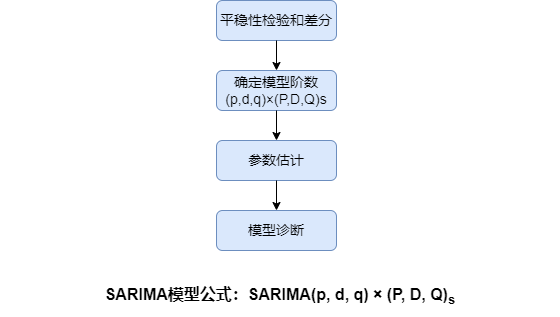
\includegraphics[width=0.75\linewidth]{figure/SARIMA_formula.png}
    \caption{SARIMA模型流程图}
    \label{fig:SARIMA模型流程图}
\end{figure}

其数学表达式可以表示为:

\[
\Phi_P(B^s) \, \phi_p(B) \, (1-B)^d \, (1-B^s)^D \, X_t \;=\; \Theta_Q(B^s) \, \theta_q(B) \, \varepsilon_t,
\]

其中,\( B \) 表示滞后算子,\( s \) 为周期长度,\( d \) 和 \( D \) 分别代表非季节性和季节性差分次数,用以消除时间序列中的趋势和季节性成分;\( \phi_p(B) \) 与 \( \Phi_P(B^s) \) 分别为非季节性及季节性自回归系数多项式;\( \theta_q(B) \) 与 \( \Theta_Q(B^s) \) 分别为非季节性及季节性移动平均系数多项式;\( \varepsilon_t \) 表示白噪声序列。

SARIMA模型的核心在于利用差分运算去除原始序列中的趋势和季节性成分,再辅以自回归和移动平均结构对去趋势后的数据进行建模,从而实现对具有明显季节性模式的数据进行精准预测. 然而,虽然SARIMA模型在捕捉季节性规律方面具有较强优势,但其在对非线性和复杂模式数据的建模能力上存在局限,因此在面对非线性特征较为显著的时间序列时,可考虑结合其他非线性模型或深度学习方法以提升预测效果。

在实际应用过程中,参数选择尤为关键,通常首先利用自相关函数(ACF)及偏自相关函数(PACF)图进行初步参数估计,随后再通过网格搜索等优化技术,结合信息准则(如AIC、BIC)对模型进行进一步调整和确认.

\section{LSTM模型}

LSTM(长短时记忆网络)模型是深度学习领域中专为时间序列数据建模而设计的一种递归神经网络(RNN)。相比于传统RNN,LSTM通过引入记忆单元(Cell State)和三个门控机制(遗忘门、输入门和输出门),有效缓解了长时间依赖问题中常见的梯度消失或梯度爆炸问题,从而更好地捕捉数据中的非线性关系。其模型结构图如图\ref{fig:LSTM模型结构图}所示。

\begin{figure}[H]
    \centering
    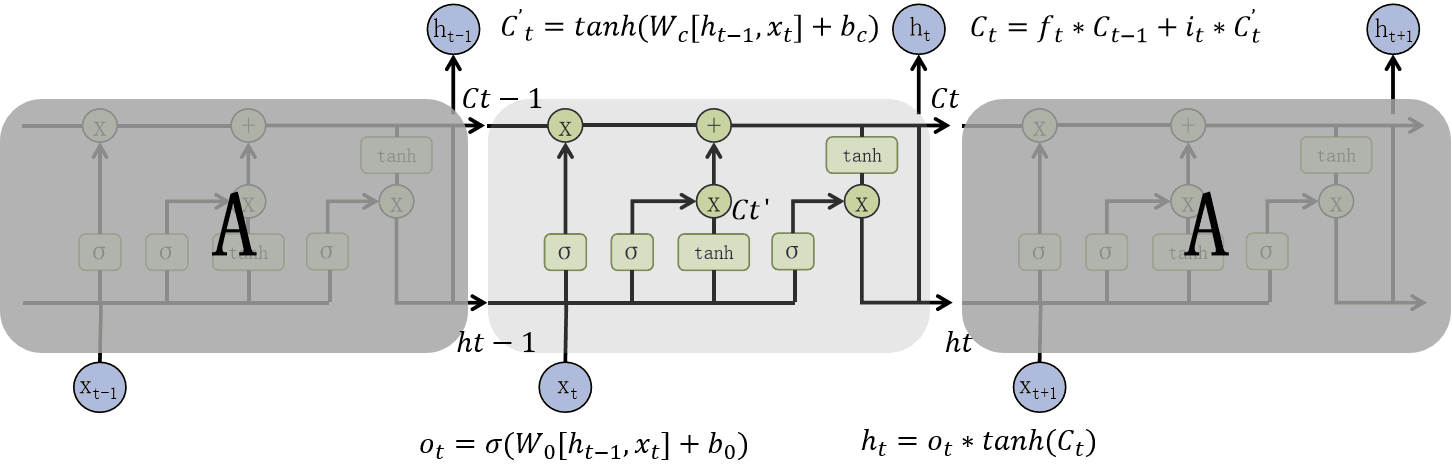
\includegraphics[width=1\linewidth]{figure/LSTM模型结构图.png}
    \caption{LSTM模型结构图}
    \label{fig:LSTM模型结构图}
\end{figure}

其工作机制可以概述如下:

首先,遗忘门决定了哪些历史信息需要被遗忘,其数学表达式为:
\[
f_t = \sigma\Big(W_f\big[h_{t-1},\,x_t\big] + b_f\Big).
\]

其次,输入门负责选择性地更新当前时间步的信息,同时生成候选记忆单元状态:
\[
i_t = \sigma\Big(W_i\big[h_{t-1},\,x_t\big] + b_i\Big), \quad 
C'_t = \tanh\Big(W_C\big[h_{t-1},\,x_t\big] + b_C\Big).
\]

然后,通过结合遗忘门和输入门的输出,更新记忆单元状态:
\[
C_t = f_t \ast C_{t-1} + i_t \ast C'_t.
\]

最后,输出门决定了当前时间步的隐藏状态,其计算过程如下:
\[
o_t = \sigma\Big(W_o\big[h_{t-1},\,x_t\big] + b_o\Big), \quad 
h_t = o_t \ast \tanh(C_t).
\]

LSTM模型因其强大的非线性建模能力,已被广泛应用于金融市场预测、流量预测、气象数据分析等任务。特别地,LSTM的引入有效解决了SARIMA模型在处理非线性问题上的不足,使其在捕捉复杂时间序列中的趋势反转和波动性变化方面表现出色。

总之,LSTM不仅在理论上为序列建模提供了有力的支持,而且在实际应用中,凭借其对非线性特征的高效捕捉能力,为解决SARIMA模型非线性局限性提供了重要补充。

\section{SARIMA-LSTM残差堆叠模型}

SARIMA-LSTM残差堆叠模型\cite{dubey2021study}是一种集成方法,通过组合传统的SARIMA模型和深度学习中的LSTM模型,实现对时间序列数据中线性及非线性成分的联合建模。其模型流程图如\ref{fig:SARIMA_LSTM残差堆叠模型流程图}所示。

\begin{figure}[H]
    \centering
    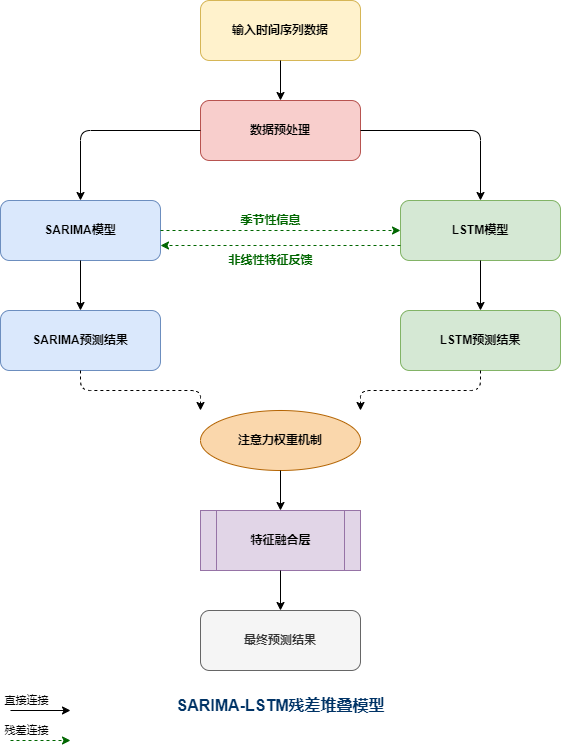
\includegraphics[width=0.6\linewidth]{figure/SARIMA_LSTM.png}
    \caption{SARIMA-LSTM残差堆叠模型流程图}
    \label{fig:SARIMA_LSTM残差堆叠模型流程图}
\end{figure}

首先,利用SARIMA模型对序列中的趋势、季节性以及其他线性模式进行捕捉,从而获得线性部分的预测值。设原始序列为 \(X_t\),经过SARIMA模型预测得到的线性部分为 \(\hat{X}_t^{\text{SARIMA}}\),残差部分可定义为
\[
e_t = X_t - \hat{X}_t^{\text{SARIMA}}.
\]
由于SARIMA模型在处理非线性和复杂动态特征上存在一定局限性,因此采用LSTM模型对预测残差进行建模,挖掘数据中潜在的非线性信息。LSTM模型通过其记忆单元及门控机制,能够捕捉长距离依赖关系和瞬时变化,从而对残差序列进行有效预测,得到 \(\hat{e}_t\)。

最终,模型将SARIMA的预测结果与LSTM对残差的预测结果相结合,形成最终的预测值:
\[
\hat{X}_t = \hat{X}_t^{\text{SARIMA}} + \hat{e}_t.
\]


这种残差堆叠方法既保留了SARIMA在捕捉长期趋势与周期性变化方面的优势,又利用LSTM弥补了对非线性和局部复杂模式的建模不足,从而提升整体预测精度。模型训练过程中,通常先对SARIMA模型进行参数估计和拟合,在确定线性部分后,再对LSTM网络进行残差序列的训练优化,确保两部分模型各自发挥专长。模型预测时,可先用SARIMA获得初步预测,再计算生成残差序列,并将其输入LSTM进行调整和修正,最后输出融合后的预测结果。
\chapter{背景}  
\label{chapter:introduction}  

在当今全球科技飞速发展的背景下,科技创新已成为推动社会进步与国家发展的核心动力。正如习近平总书记所指出的:“科技创新是发展新质生产力的核心要素。”科技创新不仅为经济增长注入活力,更为提升国家综合竞争力奠定了坚实基础。

根据国家统计局发布的报告,创新指数体系涵盖四大类与二十个小类指标,全面覆盖创新活动的各个维度(见表\ref{创新指数构成表_上}和表\ref{创新指数构成表_下})。该指标体系为深入分析国家创新能力提供了科学依据,同时也为我们评估科技前沿动态提供了可靠的数据支撑。

\begin{table}[H]
\centering
\caption{创新指数构成表(上)}
\begin{tabular}{lll}
\toprule
\textbf{分领域} & \textbf{指标名称} & \textbf{占比} \\
\midrule
\multirow{5}{*}{创新环境(1/4)} 
    & 1.1 每万人就业人员中大专及以上学历人数 & 1/5 \\
    & 1.2 人均GDP & 1/5 \\
    & 1.3 理工类毕业生占适龄人口比重 & 1/5 \\
    & 1.4 科技拨款占财政拨款比重 & 1/5 \\
    & 1.5 享受加计扣除减免税企业所占比重 & 1/5 \\
\midrule
\multirow{4}{*}{创新投入(1/4)} 
    & 2.1 每万人R\&D人员全时当量 & 1/4 \\
    & 2.2 R\&D经费占GDP比重 & 1/4 \\
    & 2.3 基础研究人员人均经费 & 1/4 \\
    & 2.4 企业R\&D经费占营业收入比重 & 1/4 \\
\midrule
\multirow{4}{*}{创新产出(1/4)} 
    & 3.1 每万人科技论文数 & 1/4 \\
    & 3.2 每万名R\&D人员高价值发明专利拥有量 & 1/4 \\
    & 3.3 拥有注册商标企业所占比重 & 1/4 \\
    & 3.4 技术市场成交合同平均金额 & 1/4 \\
\bottomrule
\label{创新指数构成表_上}
\end{tabular}
\end{table}

\begin{table}[H]
\centering
\caption{创新指数构成表(下)}
\begin{tabular}{lll}
\toprule
\textbf{分领域} & \textbf{指标名称} & \textbf{占比} \\
\midrule
\multirow{5}{*}{创新成效(1/4)} 
    & 4.1 新产品销售收入占营业收入比重 & 1/5 \\
    & 4.2 高新技术产品出口额占货物出口额比重 & 1/5 \\
    & 4.3 专利密集型产业增加值占GDP比重 & 1/5 \\
    & 4.4 “三新”经济增加值占GDP比重 & 1/5 \\
    & 4.5 全员劳动生产率 & 1/5 \\
\bottomrule
\label{创新指数构成表_下}
\end{tabular}
\end{table}

党的十四届全国人大三次会议审议通过了一系列旨在推动科技创新、促进产业升级和深化社会改革的重要政策,充分彰显了战略转型的坚定决心。特别是在政府工作报告中提出的“人工智能+”行动计划,标志着我国在人工智能领域的战略部署迈入新阶段。

此外,会议还强调,社会改革应与科技进步协同推进,尤其是在教育体系改革与人才培养机制建设方面。随着人工智能、机器人、大数据等前沿技术不断取得突破,传统就业结构与职业模式正经历深刻变化。大会明确提出,要加快教育改革步伐,着力培养符合新时代要求的复合型人才,这既是应对产业结构变迁与劳动力市场调整的必要之举,也是实现社会可持续发展的根本保障。

在深入贯彻创新驱动发展战略的背景下,本文将围绕教育、企业、就业及国际竞争力等关键领域,基于国家政策导向与科技发展趋势展开多角度分析\cite{chen2021beyond}。为明确研究方向,本文通过词云技术对政策文本进行可视化处理,为下文研究提供了理论依据与分析线索(见图\ref{fig:词云})。

\begin{figure}[H]
    \centering
    
\includegraphics[width=0.5\linewidth]{figure/wordcloud_output.png}
    \caption{政策关键词词云图}
    \label{fig:词云}
\end{figure}

从词云图中可以看出,国家政策密切聚焦于教育体系优化、企业创新能力建设、人才结构转型与国际竞争力提升等核心议题。不仅反映了当前社会关注的重点方向,也为后续章节的深入探讨提供了清晰的研究主线,力求揭示国家政策与科技发展之间的互动机制,以及其在推动社会变革中的深层作用。


\chapter{教育发展}
\label{chapter:Education}

习近平总书记深刻指出:“教育、科技、人才是全面建设社会主义现代化国家的基础性、战略性支撑。”这句话为新时代我国教育与科技的协同发展提供了战略指导。

在科技创新浪潮席卷全球的当下,教育不仅肩负着培养创新型人才的重要使命,更是推动科技进步的关键力量。十四届全国人大三次会议进一步强调,教育要与科技创新深度融合,依托人工智能等前沿技术,实现个性化、精准化培养,使得教育更具个性化、智能化特点,同时也为人才培养提供了更为广阔的平台。

此外,科技创新在教育中的广泛应用,有望有效缩小区域间的教育差距,推动教育公平普及,为全面建设社会主义现代化国家奠定坚实基础。


\section{资金投入推动科技创新}

教育支出占 GDP 的比重是衡量一个国家对教育重视程度的重要指标,直接反映了政府对教育的战略规划,并对教育质量提升、人才培养水平产生深远影响,从而与科技创新能力和社会发展紧密相连。

基于世界银行集团《教育公共开支总额》数据集,本研究绘制了各国教育支出占GDP的百分比变化趋势”折线图(见图\ref{01各国教育支出占GDP的百分比变化趋势图})。该图直观展示了各国教育支出占 GDP 比重的变化轨迹,为分析各国教育投入动态和政策效果提供了有力依据。

\begin{figure}[H]
    \centering
    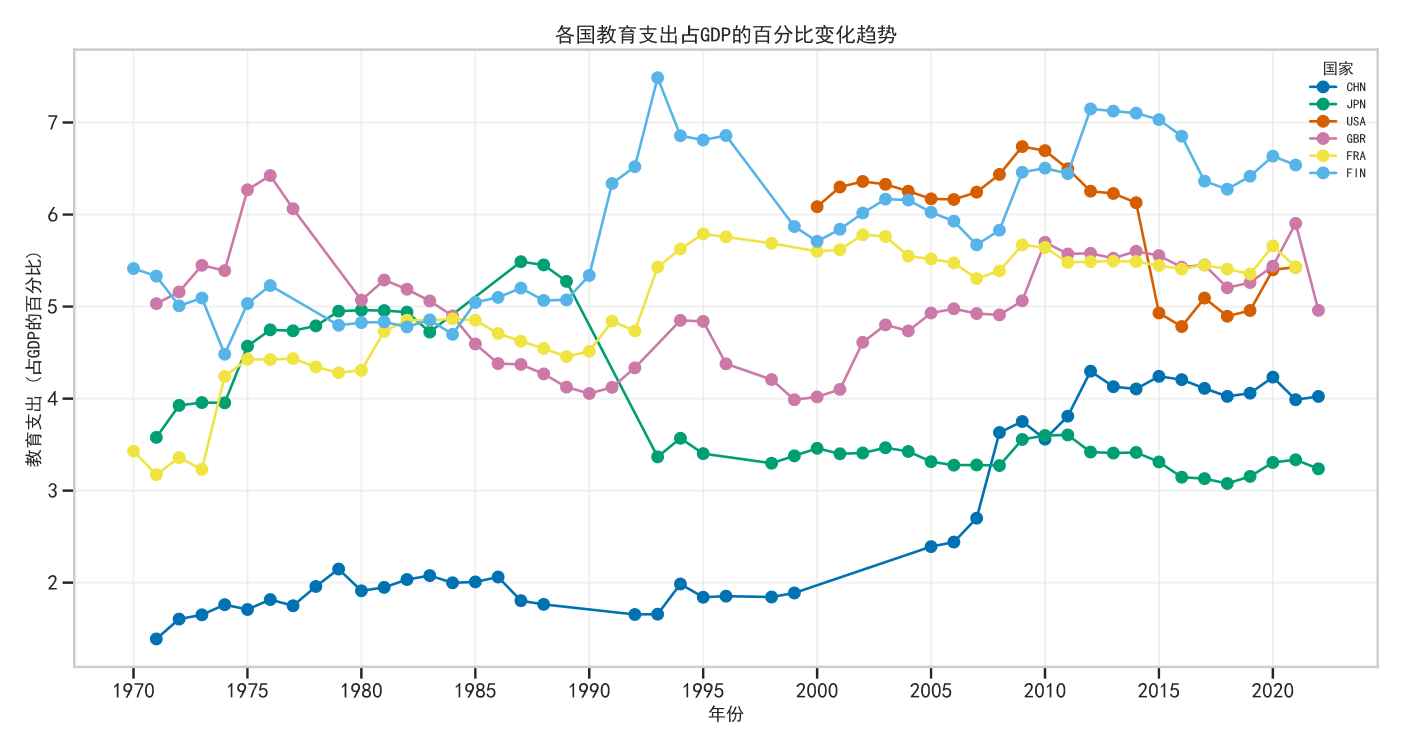
\includegraphics[width=0.7\linewidth]{figure/01各国教育支出占GDP的百分比变化趋势图.png}
    \caption{各国教育支出占GDP的百分比变化趋势图}
    \label{01各国教育支出占GDP的百分比变化趋势图}
\end{figure}

从图表中可以看出,中国的教育支出占GDP比例呈现明显上升趋势\cite{huang2021education},然而与其他国家相比仍有提升空间。具体来看,自2000年以来,中国的教育支出占比迅速攀升,尤其在2008年,即汶川地震后,出现了显著增长。这一现象可能归因于灾后学校重建、农村义务教育保障工程以及职业和高等教育的大规模扩招等多重因素共同作用。
\subsection{研究与试验发展经费支出趋势}
高等学校研究与试验发展(R\&D)经费支出的变化趋势,是衡量一国高等教育科研能力和创新投入的重要指标。基于国家统计局《高等学校科技活动情况》数据集,本研究绘制了“高等学校研究与试验发展经费支出变化趋势”折线图(见图\ref{fig:02高等学校研究与试验发展经费支出变化趋势图}),直观展示了各项经费投入随时间的变动情况。

\begin{figure}[H]
    \centering
    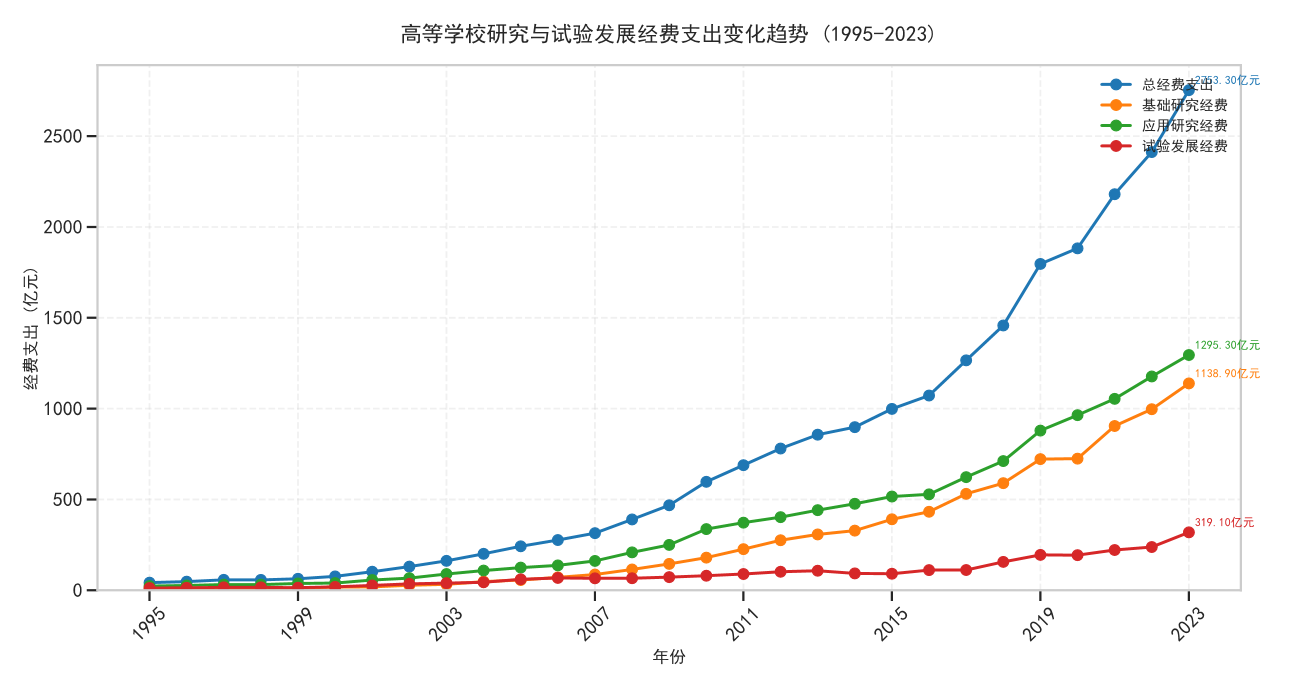
\includegraphics[width=0.8\linewidth]{figure/02高等学校研究与试验发展经费支出变化趋势图.png}
    \caption{高等学校研究与试验发展经费支出变化趋势图}
    \label{fig:02高等学校研究与试验发展经费支出变化趋势图}
\end{figure}

从图表中可以直观地看到,高等学校研究与试验发展经费的总支出呈现持续且大幅度增长的趋势\cite{Zhou2024},从1995年的不足百亿元增长至2023年的2500亿元以上。

分项经费方面,基础研究经费、应用研究经费和试验发展经费均显著增长,但其增速与占比有所差异。具体而言,试验研究经费在1995年时几乎可以忽略不计,但在2023年已达到319.1亿元;基础研究经费从较低基数逐步增长至1138.9亿元,显示出其在整体经费投入中所处的重要地位;应用研究经费的增长尤为突出,从最初的低水平跃升至1295.3亿元,稳居总经费支出的最大份额。

\subsection{研究与试验发展经费支出占比}
为更好地研究三大经费类别在整体投入中的比重变化,还绘制了“高等学校研究与试验发展经费支出占比变化”面积图(见图\ref{fig:03高等学校研究与试验发展经费支出占比变化})。

从面积图中可以看出,尽管试验发展经费的绝对数值不断攀升,但其在总体结构中的占比却出现了相对下降,这反映出当前高校在技术成果推广及实践转化方面可能存在一定的制约因素,需要进一步优化科研成果的转化机制和实践应用环节。

\begin{figure}[H]
    \centering
    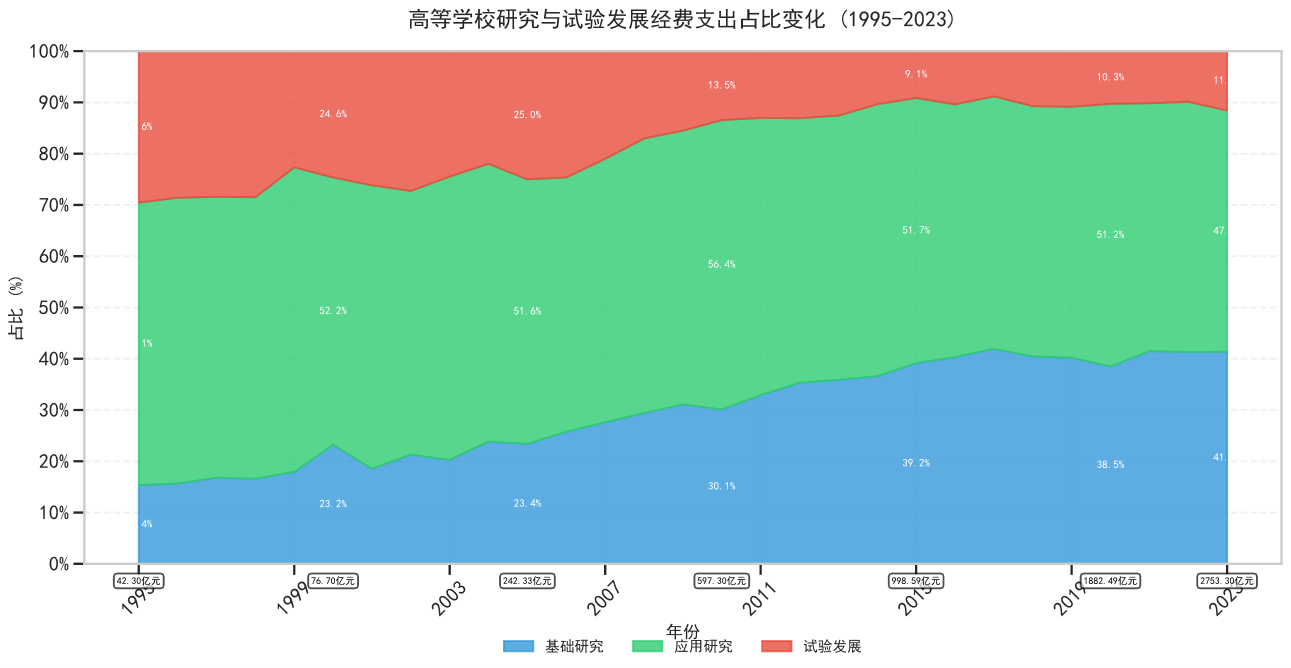
\includegraphics[width=0.7\linewidth]{figure/03高等学校研究与试验发展经费支出占比变化.png}
    \caption{高等学校研究与试验发展经费支出占比变化图}
    \label{fig:03高等学校研究与试验发展经费支出占比变化}
\end{figure}

这一现象表明,尽管高校科研经费整体快速增长,但在投入结构调控方面仍有优化空间。基础研究稳步上升显示出原始创新的重要性;而应用研究经费占比高,表明高校正加快成果转化。但试验发展经费尽管总额不断增加,其相对占比下降,暗示在科研成果实际应用和技术试验环节仍存在瓶颈,亟需完善相关政策机制。


\section{科技创新引领教育发展}

高校科研产出是衡量学术创新水平和科研能力的重要指标,其核心涵盖科研项目数量、科技论文数量以及专利授权数。基于国家统计局《高等学校科技活动情况》数据集,本研究绘制了“高校科研产出指标趋势对比与预测”折线图,并运用融合模型对未来趋势进行预测(见图\ref{fig:04高校科研产出指标趋势对比与预测图})。

\begin{figure}[H]
    \centering
    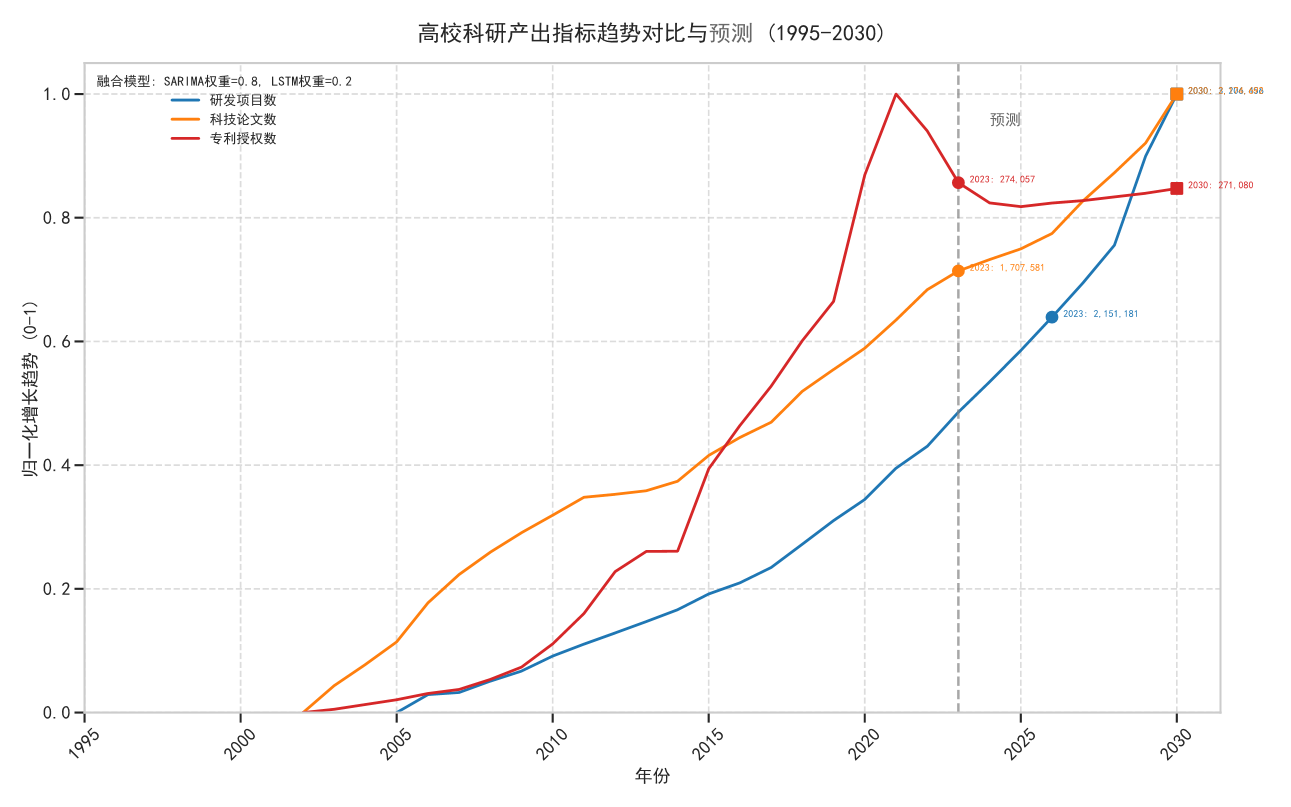
\includegraphics[width=0.7\linewidth]{figure/04高校科研产出指标趋势对比与预测图.png}
    \caption{高校科研产出指标趋势对比与预测图}
    \label{fig:04高校科研产出指标趋势对比与预测图}
\end{figure}

历史数据表明,科研项目数、科技论文数和专利授权数均显著增长,但各自阶段和增速不同。科研项目数自1995年稳步上升,至2023年达2,151,181,预计2030年将达3,206,458;科技论文数在2005–2015年间迅速攀升,至2023年达1,707,581,预计2030年将突破2,271,080;专利授权数虽波动较大(2020–2023年曾大幅下滑),但2010–2020年增速显著,2023年已达274,057,预计2030年将增至330,458。

近年来,中国政策逐步向质量导向转变,重点提升发明专利的审查标准,同时对实用新型和外观设计专利进行调整,2023年这两类专利分别下降了25.5\%和11.5\%。此外,“十四五”规划期间逐步取消专利补贴,可能进一步降低高校在低质量专利申请方面的积极性。

总体来看,科研项目数的稳步增长彰显了高校在科研投入和项目立项方面的提升;科技论文数的快速上升反映了学术影响力和国际合作的深化;而专利授权数的波动则既显示突破也暴露挑战。展望2030年,高校科研产出要在保持投入的同时,优化资源配置、加强国际合作、推动成果产业化,从而巩固其全球科技竞争地位.

\section{社会变革提供资金投入}
为探讨社会变革对未来科技创新的反作用,本研究基于前文对高校研究与试验发展经费未来五年走势的预测数据,绘制了“高等学校经费支出融合预测”折线图(见图\ref{fig:05高等学校研究与试验发展经费支出融合预测}),直观展示了未来经费支出的发展趋势。

\begin{figure}[H]
    \centering
    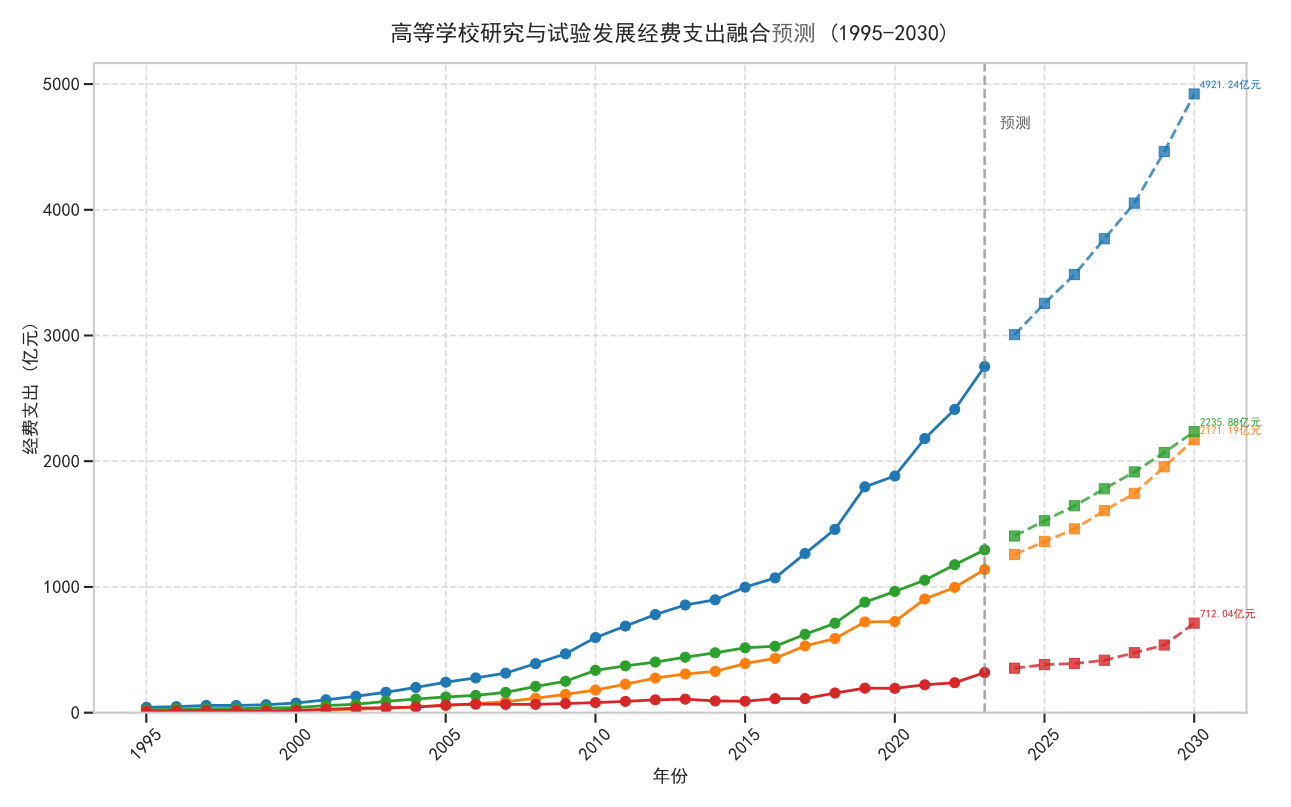
\includegraphics[width=0.7\linewidth]{figure/05高等学校研究与试验发展经费支出融合预测.png}
    \caption{高等学校研究与试验发展经费支出融合预测}
    \label{fig:05高等学校研究与试验发展经费支出融合预测}
\end{figure}

从实际数据来看,1995年至2023年间,高校科研总经费经历了指数级增长,从不足百亿元跃升至约3000亿元,预计到2030年将突破4900亿元。基础研究经费增长稳健,在极低基数的基础上迅速攀升至2023年的2171.19亿元,并预计2030年达到约2235.88亿元;应用研究经费亦持续稳步上升,2023年约为1500亿元,预测2030年将突破1700亿元。相比之下,试验发展经费虽然也呈现增长态势,但增速相对较小,2023年达到712.04亿元,预计2030年将接近800亿元。

具体的预测数据如表\ref{高校经费支出融合预测值(2024--2030)数据汇总}所示。

\begin{table}[H]
  \centering
  \caption{高校经费支出融合预测值(2024--2030)数据汇总表}
  \begin{minipage}[t]{0.48\textwidth}
    \centering
    \caption*{(a) 总经费支出预测(2024--2030)}
    \vspace{0.5em}
    \begin{tabular}{lc}
      \toprule
      年份 & 经费(亿元) \\
      \midrule
      2024 & 3006.26 \\
      2025 & 3255.37 \\
      2026 & 3484.90 \\
      2027 & 3769.74 \\
      2028 & 4052.68 \\
      2029 & 4463.49 \\
      2030 & 4921.24 \\
      \bottomrule
    \end{tabular}
  \end{minipage}
  \hfill
  \begin{minipage}[t]{0.48\textwidth}
    \centering
    \caption*{(b) 基础研究经费预测(2024--2030)}
    \vspace{0.5em}
    \begin{tabular}{lc}
      \toprule
      年份 & 经费(亿元) \\
      \midrule
      2024 & 1258.12 \\
      2025 & 1362.15 \\
      2026 & 1461.68 \\
      2027 & 1607.25 \\
      2028 & 1744.18 \\
      2029 & 1956.19 \\
      2030 & 2171.19 \\
      \bottomrule
    \end{tabular}
  \end{minipage}
  
  \vspace{1em}
  
  \begin{minipage}[t]{0.48\textwidth}
    \centering
    \caption*{(c) 应用研究经费预测(2024--2030)}
    \vspace{0.5em}
    \begin{tabular}{lc}
      \toprule
      年份 & 经费(亿元) \\
      \midrule
      2024 & 1405.42 \\
      2025 & 1526.58 \\
      2026 & 1645.90 \\
      2027 & 1781.00 \\
      2028 & 1914.91 \\
      2029 & 2068.88 \\
      2030 & 2235.88 \\
      \bottomrule
    \end{tabular}
  \end{minipage}
  \hfill
  \begin{minipage}[t]{0.48\textwidth}
    \centering
    \caption*{(d) 试验发展经费预测(2024--2030)}
    \vspace{0.5em}
    \begin{tabular}{lc}
      \toprule
      年份 & 经费(亿元) \\
      \midrule
      2024 & 353.74 \\
      2025 & 382.13 \\
      2026 & 391.36 \\
      2027 & 416.77 \\
      2028 & 476.90 \\
      2029 & 538.18 \\
      2030 & 712.04 \\
      \bottomrule
    \end{tabular}
  \end{minipage}
  
  \label{高校经费支出融合预测值(2024--2030)数据汇总}
\end{table}

高校科研经费的迅猛增长彰显了国家在科技创新领域持续加大投入,助推了高校科研能力的提升。基础研究经费以最快增速和显著占比增长,反映出高校在原始创新方面的加大投入,与国家对基础学科和前沿技术的重视相契合;应用研究经费的稳步上升突显了高校在解决实际问题和技术转化中的关键作用;而试验发展经费增长较缓,则表明技术应用和产业化领域仍需深化产学研合作。

总体来看,高校科研经费的逐年增长既验证了国家科技创新战略的成效,也凸显了高校在基础研究、应用研究和试验发展中的关键地位。未来,高校应在持续强化基础研究的同时,通过优化资源配置和深化产学研融合,提升科研质量和技术转化效率,从而在全球科技竞争中稳固并提升自身优势。

\chapter{赋能企业结构变革}
\label{chapter:Enterprise}
习近平总书记强调科技创新在发展新质生产力中的核心地位,两会也着重提出推进 “人工智能 +” 行动。在此背景下,科技创新(人工智能)作用于教育所培养出的创新型人才,正从多方面深刻影响着企业结构。

\section{风险投资金额注入企业科技创新}
风险投资(Venture Capital,VC)是推动技术创新与经济增长的关键动力,其发展水平在一定程度上反映了国家在创新投入与政策支持上的力度。基于和鲸平台的《主要国家历年风险投资金额》,我们展示了2000至2023年中国、日本、法国和芬兰风险投资额的走势。图表分别采用原始值和对数尺度,直观反映各国风险投资发展的动态变化(见图\ref{fig:主要国家风险投资金额趋势})。

\begin{figure}[H]
    \centering
    % 左侧图
    \begin{subfigure}[b]{0.45\linewidth} % 调整宽度为画布宽度的45%
        \centering
        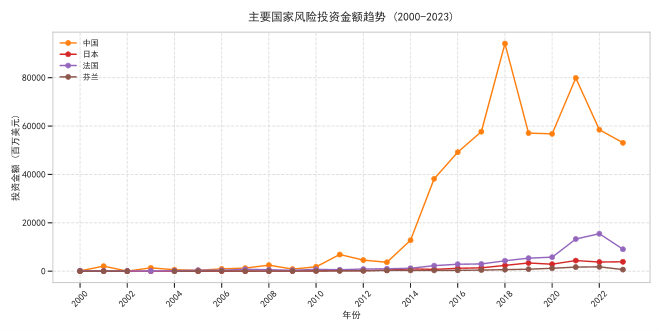
\includegraphics[width=\linewidth]{figure/07主要国家风险投资金额趋势.png}
        \caption{风险投资金额\_原始趋势}
        \label{fig:风险投资金额_原始趋势}
    \end{subfigure}
    \hfill % 增加子图之间的间距
    % 右侧图
    \begin{subfigure}[b]{0.45\linewidth}
        \centering
        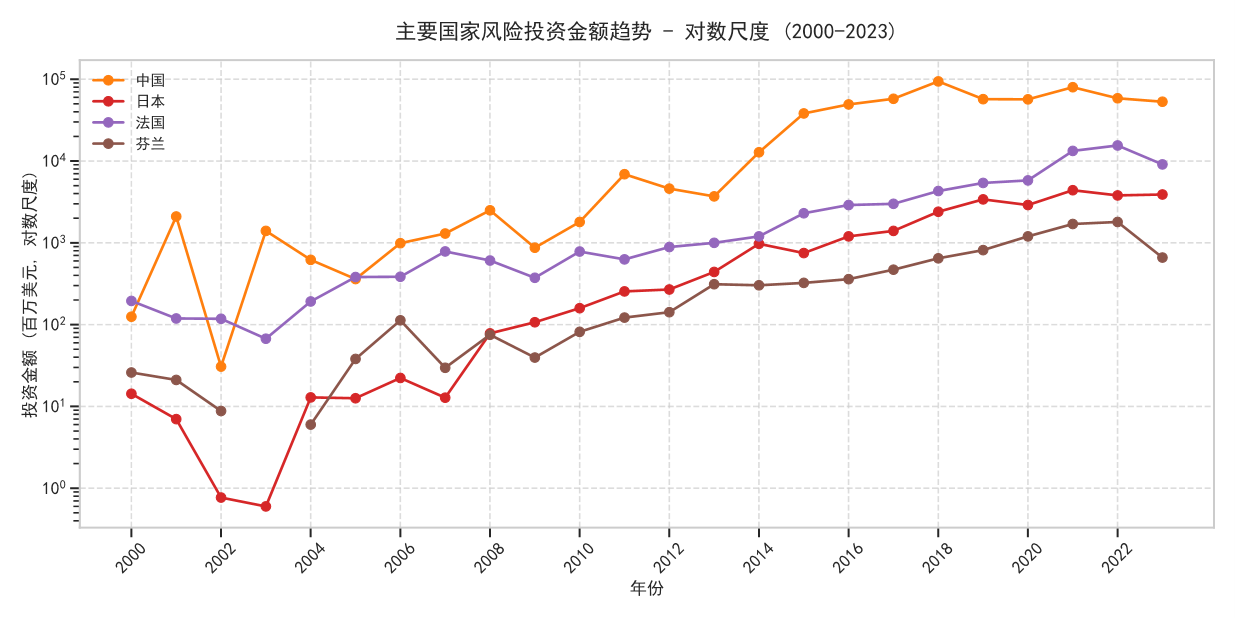
\includegraphics[width=\linewidth]{figure/06主要国家风险投资金额趋势-对数尺度.png}
        \caption{风险投资金额\_对数趋势}
        \label{fig:风险投资金额_对数趋势}
    \end{subfigure}
    \caption{风险投资金额原始趋势与对数趋势对比}
    \label{fig:主要国家风险投资金额趋势}
\end{figure}

中国在图\ref{fig:风险投资金额_原始趋势}中表现出显著的风险投资增长态势,尤其在2014至2018年期间,投资额几乎呈指数式上升,并在2018年达到近9万亿元的峰值\cite{Chen2022}。尽管自2019年后有所回落,总体投资水平依然居高不下。而图\ref{fig:风险投资金额_对数趋势}则从相对变化的角度展现了各国投资趋势,反映出各国在创新驱动经济发展中对资源配置和政策侧重点的不同。

中国的风险投资额在2014年至2018年经历了显著的快速增长,这一阶段得益于政策支持、资本市场开放以及新兴技术领域的迅速发展,从而奠定了中国在全球创新生态中的领先地位。这种大幅提升不仅彰显了中国在风险投资领域的崛起,也为未来发展提出了新的挑战,即如何在持续保持高投资额的同时,通过高效配置资源来最大化技术价值。

\section{独角兽公司发展趋势}
独角兽是指成立不到10年但估值10亿美元以上,又未在股票市场上市的科技创业公司。这些公司通常具有强大的创新能力和成长性,是新经济发展的风向标,也是新质生产力的典型代表。

\subsection{中国现存独角兽企业}
在中国现存独角兽企业部分,数量与估值的变化趋势不仅反映出创业生态环境的演变,也展示了资本市场对新兴行业的关注和投入。根据和鲸平台、睿兽分析的《主要国家独角兽公司数量》数据集,制作了“2013-2023年中国市场独角兽存续总数量变化”的柱状图和“2013-2023年中国存量独角兽平均估值变化”的折线图(见图\ref{fig:独角兽数量与估值变化})。

\begin{figure}[H]
    \centering
    % 左侧图
    \begin{subfigure}[b]{0.45\linewidth} % 调整宽度为画布宽度的45%
        \centering
        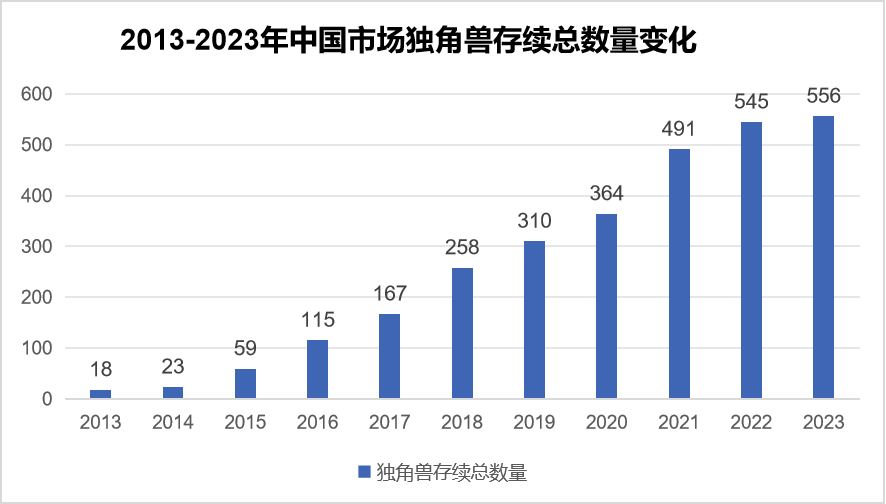
\includegraphics[width=\linewidth]{figure/08中国市场独角兽存续总数量变化.png}
        \caption{2013-2023年中国市场独角兽存续总数量变化}
        \label{fig:独角兽存续数量}
    \end{subfigure}
    \hfill % 增加子图之间的间距
    % 右侧图
    \begin{subfigure}[b]{0.45\linewidth}
        \centering
        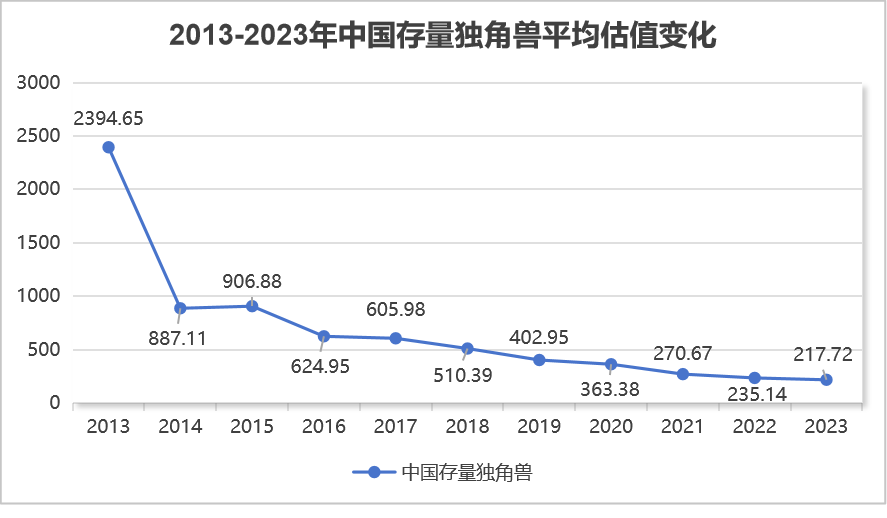
\includegraphics[width=\linewidth]{figure/09中国存量独角兽平均估值变化.png}
        \caption{2013-2023年中国存量独角兽平均估值变化}
        \label{fig:独角兽平均估值}
    \end{subfigure}
    \caption{中国市场独角兽的数量与估值变化趋势}
    \label{fig:独角兽数量与估值变化}
\end{figure}

从图\ref{fig:独角兽存续数量}可见,过去十年中国独角兽企业数量快速增长,尤其在2015至2021年间,从59家激增至491家,年均增幅明显,显示出政策支持、资本注入和技术创新共同推动了孵化能力的提升。但2022年和2023年的增速有所放缓,总量分别为545家和556家,可能与全球经济放缓及宏观环境不确定性有关。

同时,图\ref{fig:独角兽平均估值}显示,2013年至2023年间中国独角兽企业平均估值从2394.65亿元急剧下降至217.72亿元,降幅超过90\%。这可能是由于企业数量激增分散了头部优势,加之资本市场对企业盈利和可持续发展的重视,使估值标准趋于理性。

两组数据综合显示,企业数量的爆发性增长反映了创业生态活跃及资本支持力度强\cite{Xu2024},但增长放缓提示资源配置亟待优化,防止资本过度集中。其次,估值大幅下降表明市场正从“数量驱动”向“质量驱动”转变,更有利于培养具备长期竞争力的企业,同时也反映出资本对宏观经济和行业前景预期的变化。

总体来看,中国独角兽企业在近十年经历了数量激增与估值下调的现象,显示市场正从扩张向理性调整过渡。政策制定者和市场各方需更加注重支持高质量增长,通过优化资本配置、提升技术创新和推动企业可持续发展,确保企业在全球竞争中保持领先。同时,独角兽企业需从依赖高估值转变为注重核心技术和商业模式创新,以实现长期稳健发展。

\subsection{中国新晋独角兽企业}

近年来,中国现存独角兽企业数量的不断增长显示了创业生态的活跃性和资本市场的强力支持。在此基础上,深入分析新晋独角兽在各行业和重点省市的分布,有助于识别具备爆发潜力的领域和未来创新高地,从而为政策制定和资本布局提供参考。基于和鲸平台、睿兽数据集,制作了“2021-2013年中国新晋独角兽细分行业分布”的柱状图和“中国重点省市独角兽情况”的柱状折线图(见图\ref{fig:独角兽行业与区域分布}),以揭示新晋独角兽在行业和区域上的动态变化。

\begin{figure}[H]
    \centering
    % 左侧图
    \begin{subfigure}[b]{0.45\linewidth} % 调整宽度为画布宽度的45%
        \centering
        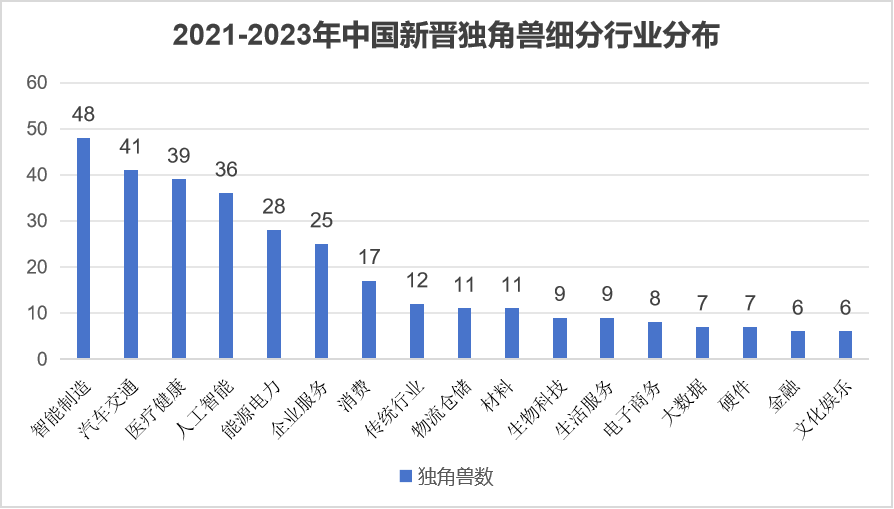
\includegraphics[width=\linewidth]{figure/10中国新晋独角兽细分行业分布.png}
        \caption{2021-2013年中国新晋独角兽细分行业分布}
        \label{fig:新晋独角兽行业分布}
    \end{subfigure}
    \hfill % 增加子图之间的间距
    % 右侧图
    \begin{subfigure}[b]{0.45\linewidth}
        \centering
        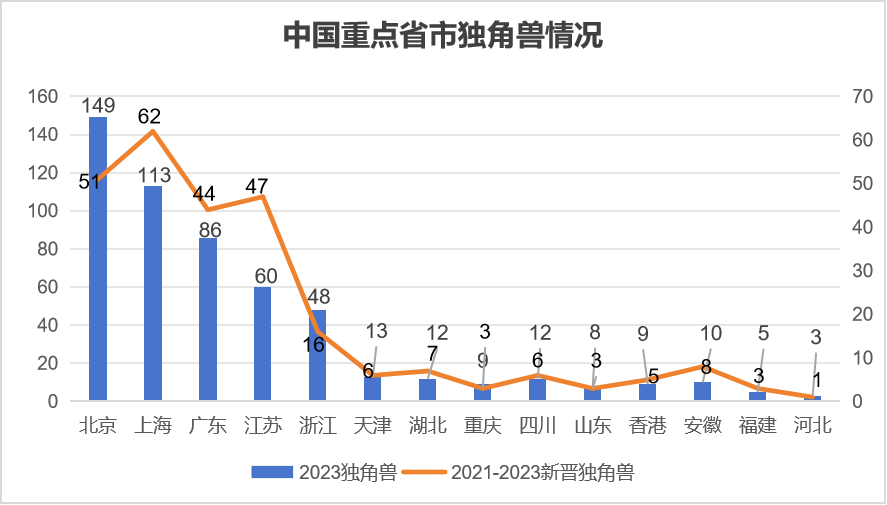
\includegraphics[width=\linewidth]{figure/11中国重点省市独角兽情况.png}
        \caption{中国重点省市独角兽情况}
        \label{fig:重点省市独角兽}
    \end{subfigure}
    \caption{中国新晋独角兽行业分布与重点省市情况对比}
    \label{fig:独角兽行业与区域分布}
\end{figure}

从图\ref{fig:新晋独角兽行业分布}中可以看出,智能制造、汽车交通和医疗健康是新增独角兽企业数量最多的三个行业,分别达到48家、41家和39家,处于主导地位。这表明,中国的独角兽企业正逐步向高端制造、生物医疗等技术密集型领域聚拢,反映出国家对战略性新兴产业的强力支持以及市场对高技术领域的投资热情。同时,人工智能、能源电力和企业服务等领域的新增独角兽数量也较为可观,进一步彰显了中国经济转型过程中对数字化、智能化和服务化发展的高度重视。

产业链与创新链的深度融合,正推动长三角地区成为中国近三年独角兽增长最快的区域。从区域分布看,独角兽企业往往集中在科研、人才、机构、企业优势明显的省市。图\ref{fig:重点省市独角兽}显示,截至2023年,北京、上海和广东分别拥有149家、113家和86家独角兽企业,遥遥领先;浙江和江苏也以60家和48家紧随其后。值得注意的是,2021年至2023年间,北京新增独角兽达51家,占全国新增比例显著,进一步巩固了其国家创新中心的地位;上海和广东分别新增62家和44家,强化了长三角和珠三角的引领作用。天津、湖北、四川等地虽然总量较少,但在新增数量上也展现出增长潜力。

未来,在确保核心区域依然保持领先优势的同时,如何进一步提升中西部及非一线城市的创新能力,将成为优化中国独角兽企业空间布局的关键。为此,建议政策制定者加大对欠发达地区创新生态的支持力度,同时持续推动高技术领域的研发投入与产业化进程,以助力中国独角兽企业迈向高质量发展。

\section{科技创新引领企业发展}
规模以上工业企业的研发活动被视为推动产业技术进步和实现经济高质量发展的关键力量。正因如此,本研究基于国家统计局和和鲸平台提供的《规模以上工业企业的科技活动基本情况》数据集,制作了“规模以上工业企业研发活动情况及预测”柱状折线图(见图\ref{规模以上工业企业研发活动情况及预测})。该图表利用融合模型预测了2004年至2030年期间企业参与研发活动的数量及其占比变化趋势,为评估工业企业未来研发投入及技术创新趋势提供了有力依据。

\begin{figure}[H]
    \centering
    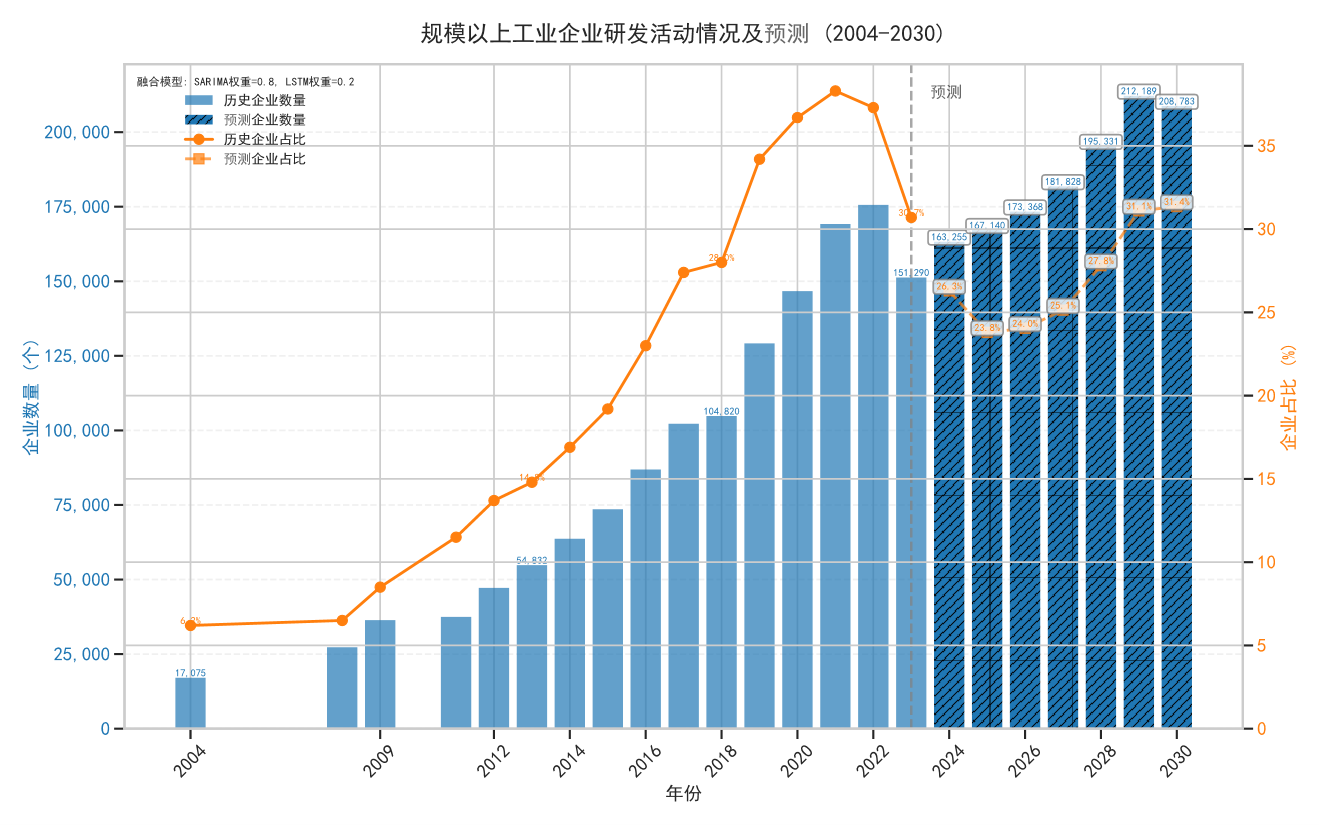
\includegraphics[width=0.7\linewidth]{figure/12规模以上工业企业研发活动情况及预测.png}
    \caption{规模以上工业企业研发活动情况及预测}
    \label{规模以上工业企业研发活动情况及预测}
\end{figure}


从2004年至2020年,规模以上工业企业参与研发活动的数量显著增长,从17,075家增加到151,290家,年均增长率较高。这显示出企业对技术创新的重视及政策对研发投入的激励作用\cite{WenZhao2021}。同时,研发活动占比由6\%上升至约30\%,表明研发已成工业企业发展的核心。值得注意的是,虽然2018年研发占比达到34\%的高点,但2020年后企业数量增速放缓,预计到2030年将达到212,189家,研发占比维持在31\%左右。这或许反映了市场成熟度、技术扩散和政策调整的影响,同时也说明了研发重心正由数量扩张转向质量提升。

未来,随着企业研发活动数量增速趋缓和占比稳定,重点应转向提升研发活动的质量与效率。建议进一步完善政策支持,鼓励高新技术企业加强基础研究与技术攻关,同时推动中小企业通过协同创新提升研发能力。此外,加强研发成果转化和应用,并完善知识产权保护机制,将有助于企业在全球竞争中保持技术优势。

\section{企业生产新产品促进市场}
随着人工智能技术的迅猛发展,其在社会生活、商业应用和产业创新中的影响不断增强。但公众对人工智能的认知与接受存在分歧,技术普及的同时也引发了隐私保护、伦理偏见和技术透明性等方面的担忧。在此背景下,人工智能的广泛应用引起了各界高度关注,尤其是生成式AI、自动化系统和智能服务的发展,既加速了技术落地,又带来了众多复杂的社会问题。基于和鲸平台的数据集,我们制作了“全球对人工智能产品与服务的看法(占比与总体百分比)——2022 VS 2023”柱状图(见图\ref{全球对人工智能产品与服务的看法(占比与总体百分比)——2022 VS 2023})。

\begin{figure}[H]
    \centering
    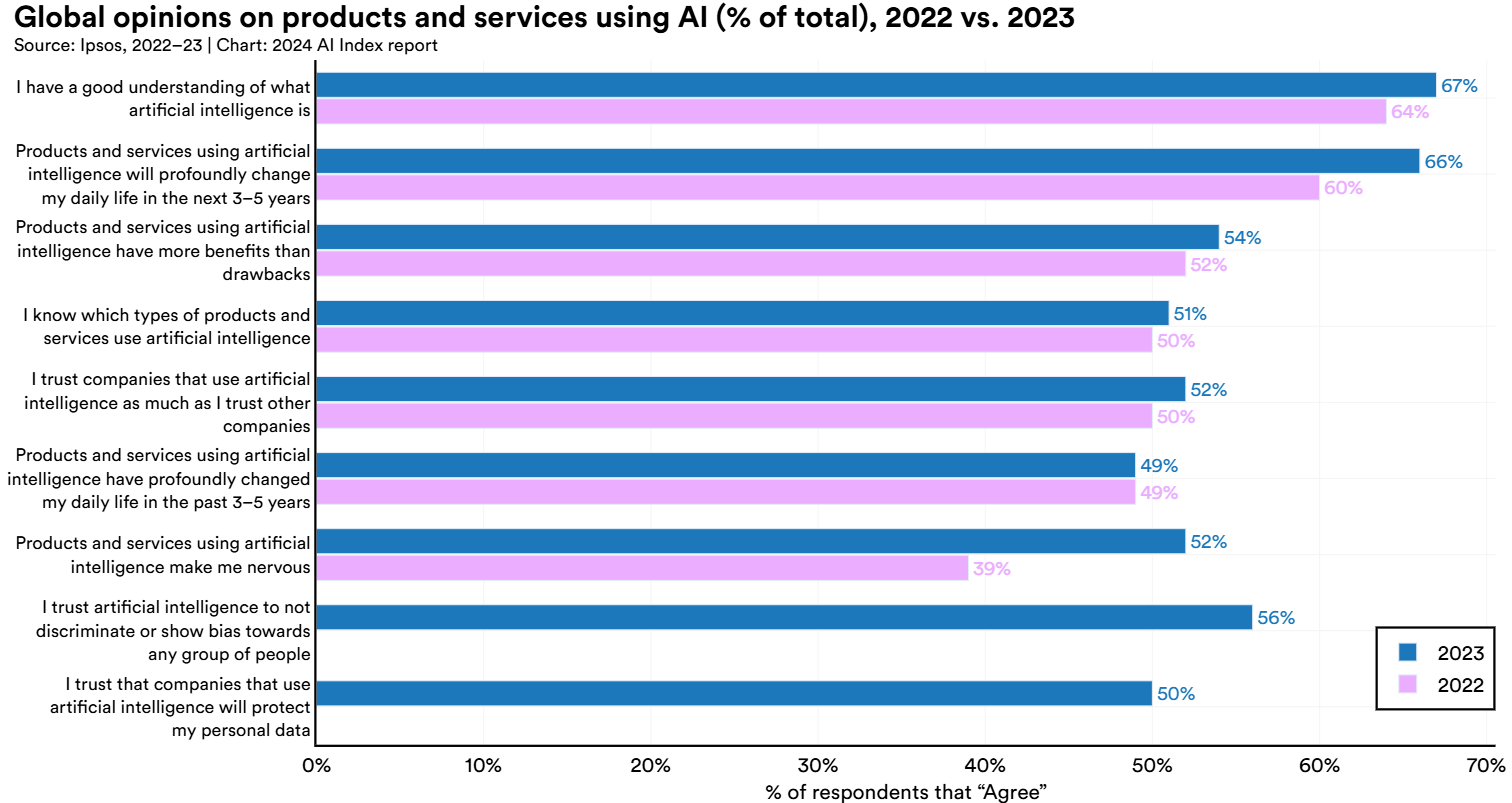
\includegraphics[width=0.7\linewidth]{figure/13全球对人工智能产品与服务的看法(占比与总体百分比)——2022 VS 2023.png}
    \caption{全球对人工智能产品与服务的看法(占比与总体百分比)——2022 VS 2023}
    \label{全球对人工智能产品与服务的看法(占比与总体百分比)——2022 VS 2023}
\end{figure}

数据显示,公众对AI的理解程度由64\%升至67\%,认为其将在未来3至5年深刻改变生活的比例由60\%增至66\%,而“好处多于缺点”的认同率由52\%小幅提升至54\%。与此同时,信任“使用AI的公司会保护个人数据”的比例维持在50\%,但感到紧张的比例却由39\%大幅上升到52\%,反映出对技术高速发展的不确定性;另外,有49\%的受访者认为AI在过去3至5年中对生活产生了深远影响,表明实际影响正在逐步累积。

综合来看,公众对人工智能的认知和接受度正在提高,体现了技术普及和广泛应用的趋势,而隐私保护和技术中立性方面的信任问题依然突出\cite{Zuiderwijk2021},伦理、偏见与监管风险引发的担忧也在增加。未来,技术提供者与政策制定者应致力于提升技术透明度、加强隐私保护和优化用户体验,同时通过科普和教育进一步普及AI知识,以构建更高的信任感,推动人工智能健康发展和广泛应用。

\section{风险投资金额注入企业科技创新}
为探讨未来社会变革对科技创新的反作用力,基于和鲸平台《主要国家历年风险投资金额》数据集,绘制了“中国风险投资金额历史数据与融合预测(2000-2030年)”折线图(如图\ref{中国风险投资金额历史数据与融合预测(2000-2030年)})。该图展示了2000年至2030年间中国风险投资金额的历史走势及融合模型的预测结果,为科学评估中国风险投资的长期发展趋势和制定相关政策提供了坚实的数据支持。

\begin{figure}[H]
    \centering
    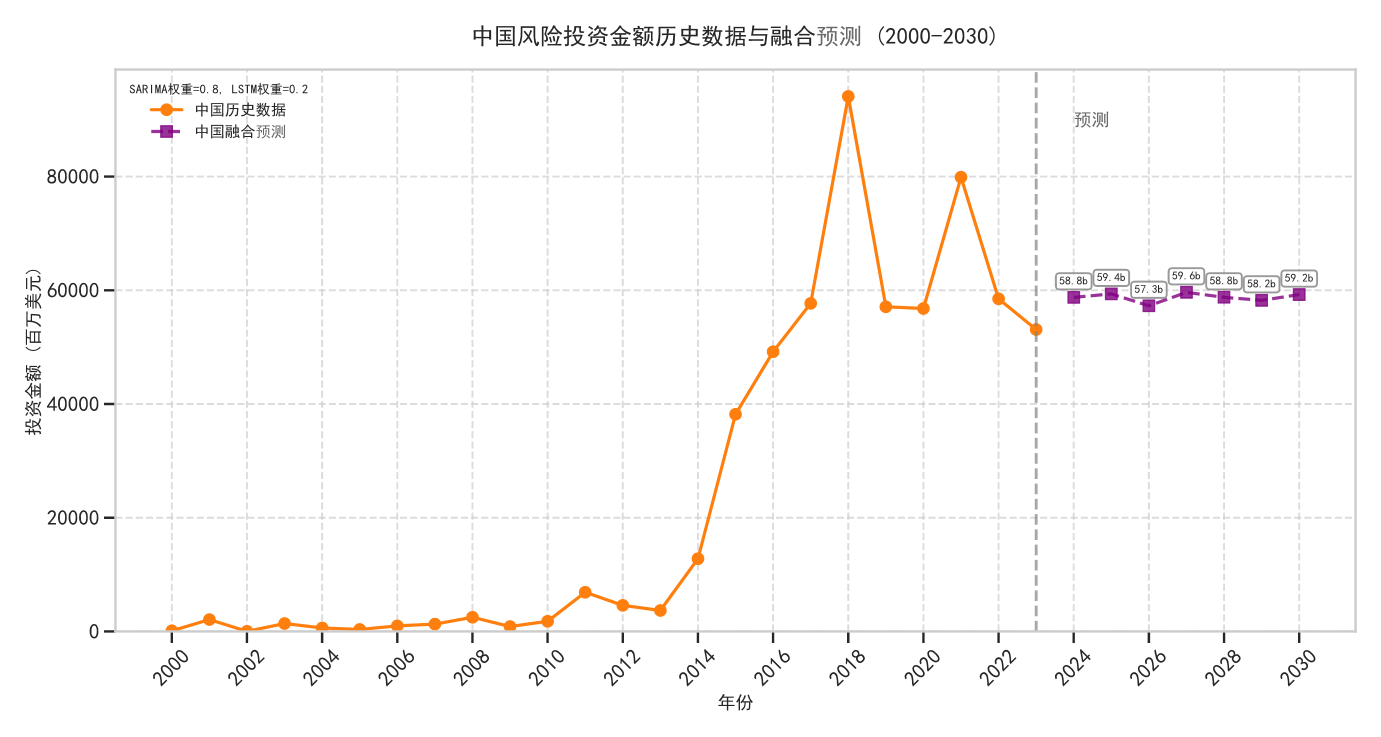
\includegraphics[width=0.7\linewidth]{figure/14中国风险投资金额历史数据与融合预测.png}
    \caption{中国风险投资金额历史数据与融合预测(2000-2030年)}
    \label{中国风险投资金额历史数据与融合预测(2000-2030年)}
\end{figure}

根据预测数据,2024年至2030年间,中国风险投资金额预计将趋于稳定,维持在约59,000百万美元左右。不过,受疫情以来市场剧烈波动的影响,该预测仍存在不确定性,可能需要结合更精确的经济学模型进行量化分析。

在未来,随着风险投资金额的稳定,投资重心将进一步转向高价值和高科技项目。为提升资本配置效率,建议政策制定者优化现有政策环境,鼓励多元化投资渠道的发展,并加大对新兴技术领域的支持力度。同时,风险投资机构应更加注重评估企业核心技术实力及长期发展潜力,推动创新生态系统的可持续发展。

\chapter{就业结构的转型}
\label{chapter:struct}
《创新发展战略》指出,国家通过大力支持创新型企业,加速科技进步和产业升级,不仅优化并提升了企业结构,也显著改变了各行业对人才的需求。随着创新型企业的崛起,对跨学科、复合型人才,尤其是具备技术开发与创新能力的高端人才的需求日益增加。在这一趋势下,企业的创业和变革成为推动就业结构调整的重要力量,不仅催生了大量与科技创新紧密相关的新兴职业,也推动劳动者技能的转型,为社会迈向更加智能化、高效化奠定了坚实基础。

\section{劳动生产率与失业人数现状}
近年来,中国的劳动生产率与失业率的波动呈现出较为复杂的变化趋势。基于CEIC的《中国劳动生产率》数据集和世界银行集团的《总失业人数(占劳动力总数的比例)(模拟劳工组织估计)》数据集,绘制出2013年至2024年间中国劳动生产率的年度变化情况(见图\ref{中国劳动生产率}),以及中国、美国、日本、英国、法国等主要国家自1990年以来的失业率对比情况(见图\ref{主要国家失业率对比})。
\begin{figure}[H]
    \centering
    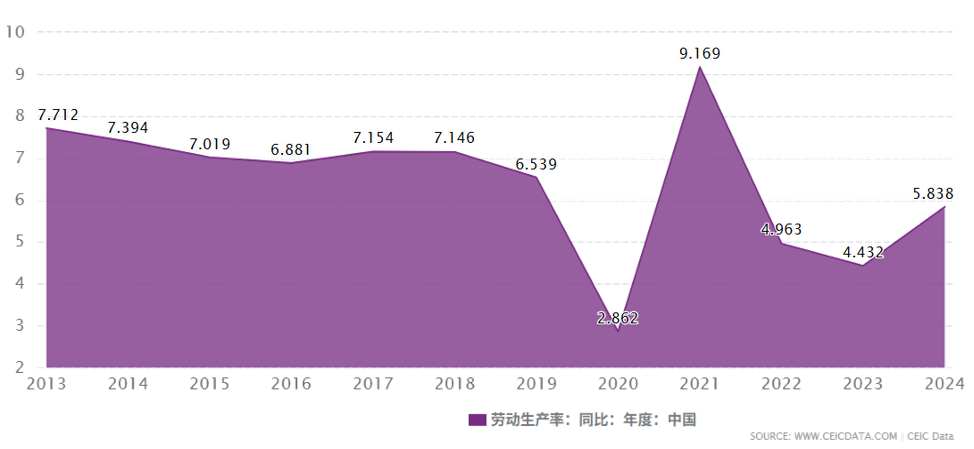
\includegraphics[width=0.7\linewidth]{figure/15中国劳动生产率.png}
    \caption{中国劳动生产率面积图}
    \label{中国劳动生产率}
\end{figure}
通过对图\ref{中国劳动生产率}的观察,可以清晰地看到中国劳动生产率这些年来波动明显,尤以2020年和2021年期间的剧烈波动为代表。数据充分表明,劳动生产率的波动受外部经济环境和国内政策的共同影响:2020年疫情对经济活动构成了巨大冲击,而2021年全球经济的复苏则带来了短期内的反弹。总体而言,尽管短期内波动较大,但在全球经济复苏及国内政策推动下,未来中国劳动生产率有望逐步进入稳定增长轨道。
\begin{figure}[H]
    \centering
    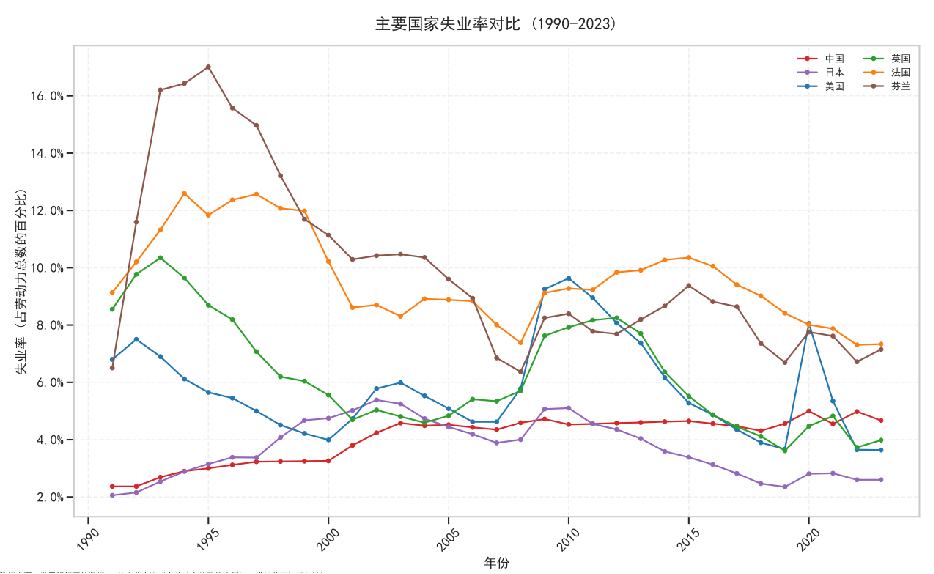
\includegraphics[width=0.7\linewidth]{figure/16主要国家失业率对比.png}
    \caption{主要国家失业率对比图}
    \label{主要国家失业率对比}
\end{figure}
同时,从图\ref{主要国家失业率对比}中可以看出,各国在不同时间段内的失业率变化各具特色。尤其是在1990年代中期和2008年全球金融危机期间,多国失业率均出现明显波动,这些波动反映了全球经济动荡对各国就业市场的深远影响。与此相比,中国的失业率总体呈现平稳上升的趋势,即使在2020年全球疫情爆发时曾短暂上升,但在政府有效政策调控下,很快得以控制,保持在较低水平,显示出较强的经济韧性与调适能力。

总体来看,劳动生产率的提升一直是中国经济转型的重要标志。与此同时,随着产业升级和自动化、智能化技术的不断推进,低技能岗位正逐步被新技术替代,导致部分领域的失业压力加大,尤其体现在年轻人和低技能工人群体中。如何在推动高技术岗位发展的同时,有效应对传统岗位的减少,是当前亟需解决的挑战。\cite{zhang2022digital}

\section{科技创新促进就业结构转型}
随着科技创新特别是人工智能、大数据、云计算等技术的普及,全球劳动市场、就业市场的结构发生了深刻变化。特别是在中国,科技创新推动了许多新兴行业的发展,尤其是在第三产业(服务业)中。传统制造业和农业中低技能岗位的减少,使得高技能岗位的需求逐步增加。

\subsection{全球人工智能岗位趋势}
AI岗位作为技术密集型职位,随着全球对人工智能技术的需求不断上升,已成为各国劳动市场中极为重要的一部分。基于和鲸平台数据集,制作出“2014-2023年各个地区人工智能(AI)相关岗位所占总岗位比例的变化情况”折线图(见图\ref{各个地区人工智能(AI)相关岗位所占总岗位比例的变换情况图})。

\begin{figure}[H]
    \centering
    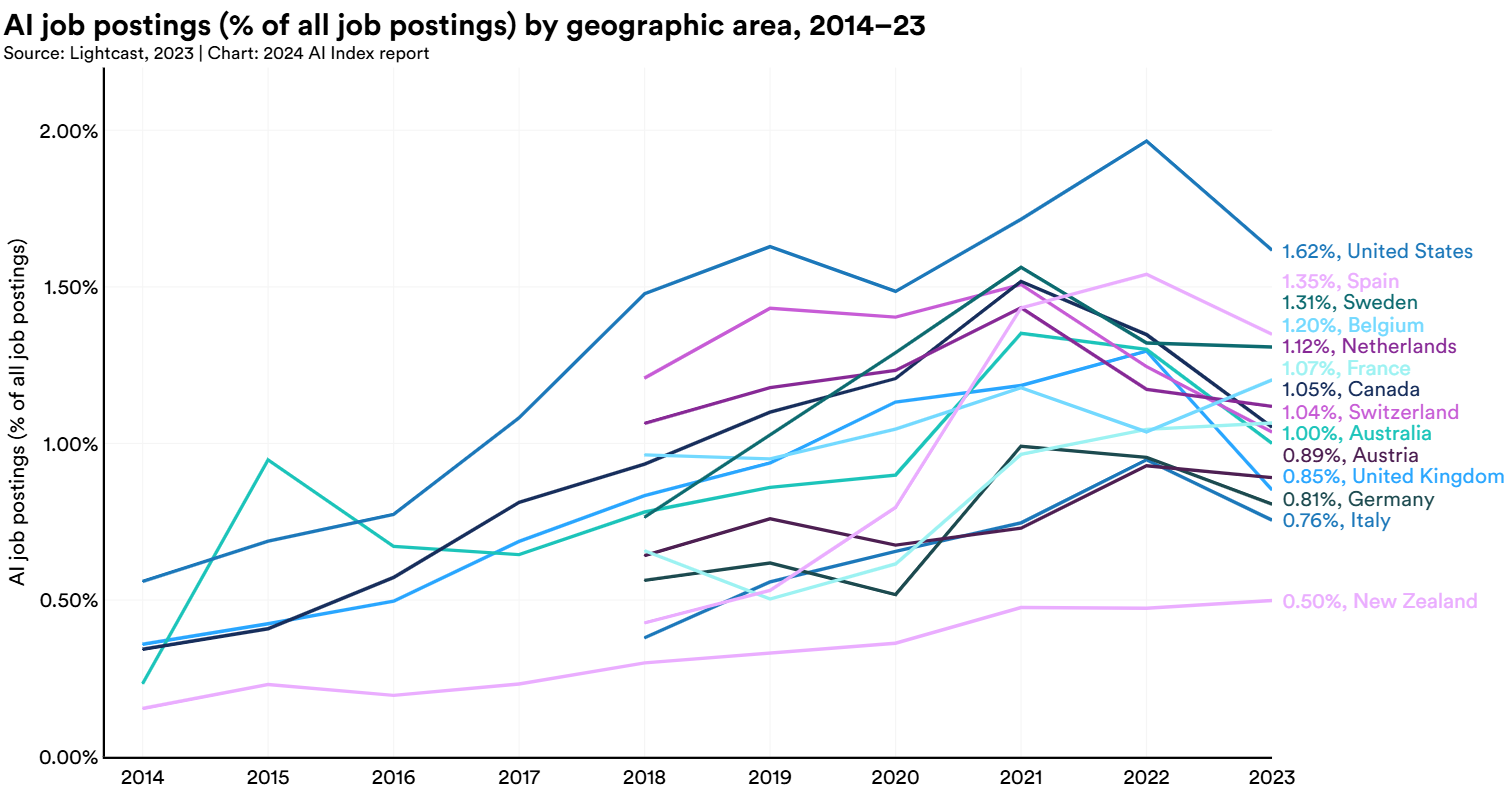
\includegraphics[width=0.7\linewidth]{figure/17各个地区人工智能(AI)相关岗位所占总岗位比例的变换情况图.png}
    \caption{各个地区人工智能(AI)相关岗位所占总岗位比例的变换情况图}
    \label{各个地区人工智能(AI)相关岗位所占总岗位比例的变换情况图}
\end{figure}

该图清晰地展示了2014年至2023年期间,各国AI岗位占比的逐年变化。全球人工智能岗位比例总体呈上升趋势,但在2023年出现了下降,这表明市场对人工智能技术的投资与需求可能正经历阶段性调整,行业不断成熟和竞争加剧使得岗位增长趋于理性。

展望未来,随着技术创新不断深入,人工智能岗位将成为全球劳动力市场的重要组成部分,尤其在高技术行业中的应用将进一步拓展。各国需要加大对AI技术研发的投入,并加强人才培养,以迎接即将到来的技术变革。\cite{wang2024impact}

\subsection{全球AI岗位发布情况}
在当前快速发展的科技环境中,人工智能(AI)正逐步改变全球劳动力市场的格局。随着AI技术的广泛应用,各组织对于AI对员工数量和工作结构的影响产生了不同的预期。根据和鲸平台数据集,展示出2023年,基于麦肯锡和公司调查数据,未来3年人工智能对组织劳动力影响的预期(见图\ref{未来3年人工智能对组织劳动力影响的预期图})。
\begin{figure}[H]
    \centering
    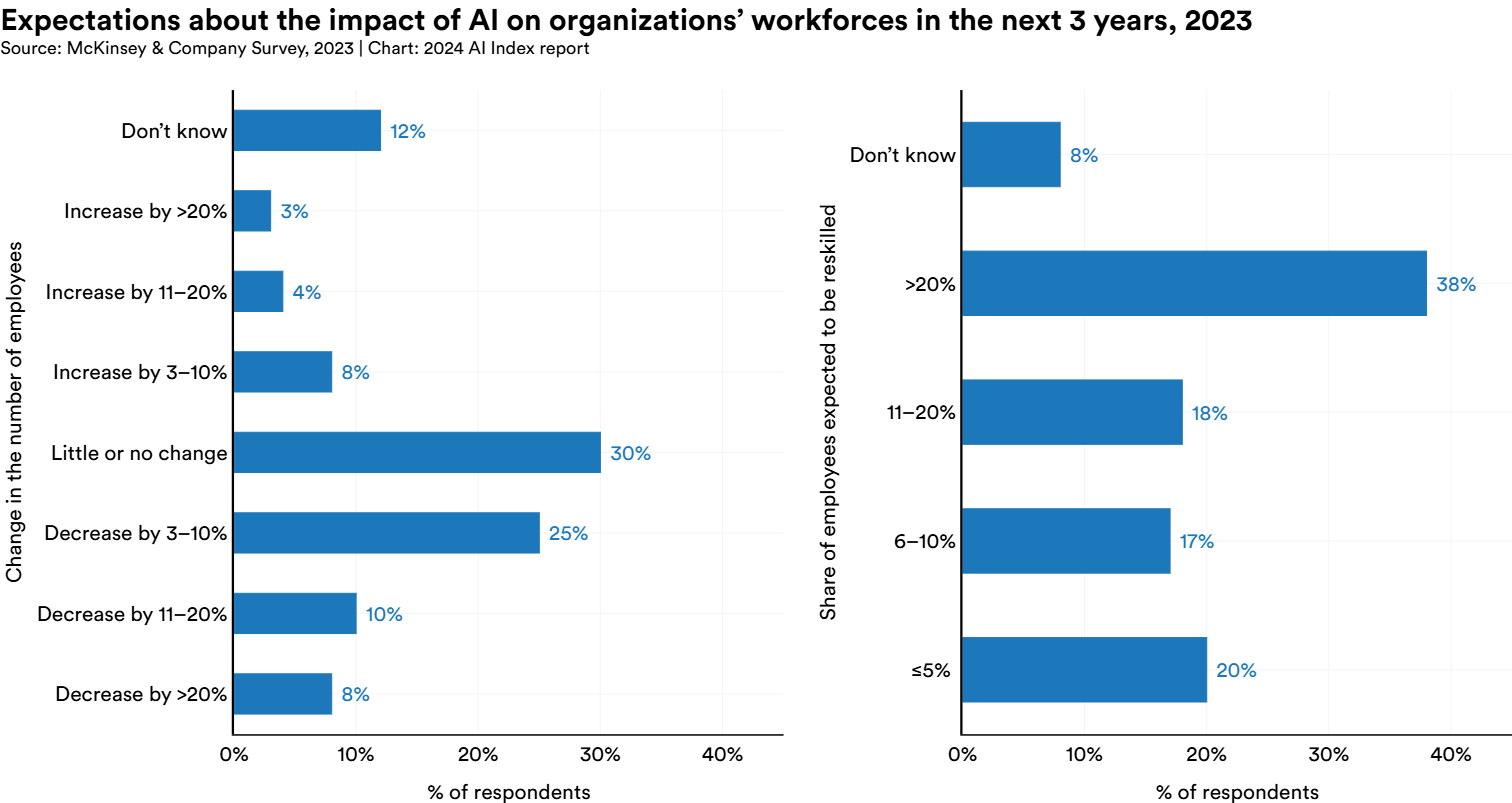
\includegraphics[width=0.7\linewidth]{figure/18未来3年人工智能对组织劳动力影响的预期图.png}
    \caption{未来3年人工智能对组织劳动力影响的预期图}
    \label{未来3年人工智能对组织劳动力影响的预期图}
\end{figure}

图表左侧展示了未来三年内,AI对员工数量变化的预期。其中有38\%的受访者认为,随着AI技术的推广,员工数量将增加超过20\%,这显示出许多企业对AI在提升劳动效率和创造就业机会方面充满信心;30\%的受访者则认为AI对员工数量的影响较小;而25\%的受访者预计,AI的应用可能使部分岗位受自动化或优化影响,导致员工数量下降3\%-10\%。

图表右侧则反映了关于AI对员工再培训需求的预期数据,38\%的受访者认为,超过20\%的员工需要接受再培训以适应技术变革,仅8\%的受访者对此持不确定态度。这表明,企业普遍认识到在AI日益普及的趋势下,员工技能升级成为必然选择。

总体而言,数据揭示了AI技术对劳动力市场的双重影响:一方面,它有望大幅提升生产力并带来更多高技能岗位;另一方面,低技能岗位可能面临被替代的风险。为此,各国企业和政府应提前制定措施,加强员工再培训和技能提升,以平衡技术进步带来的机遇和挑战。

\subsection{研发人员数量变化与科技创新推动的关系}
随着中国经济的持续增长和科技创新的不断推进,工业企业的研发投入和人才培养已成为衡量企业竞争力的重要标准、推动产业升级的关键。基于国家统计局以及和鲸平台的数据集《规模以上工业企业的科技活动基本情况》,制作出“2004-2023年中国规模以上工业企业研发人员数量的变化趋势”的柱状图(见图\ref{中国规模以上工业企业研发人员规模变化趋势图})。
\begin{figure}[H]
    \centering
    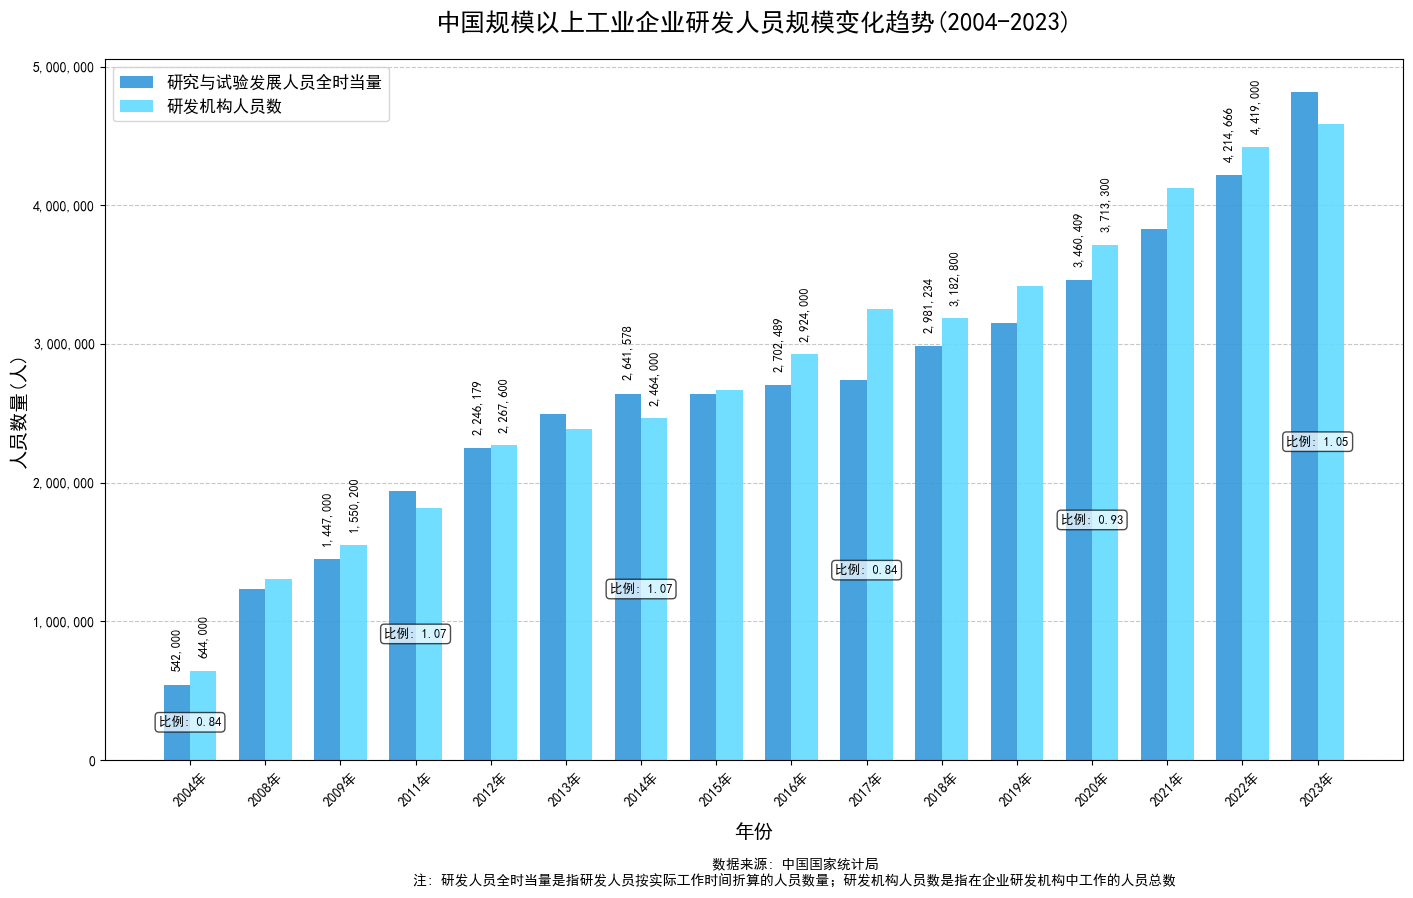
\includegraphics[width=0.6\linewidth]{figure/19中国规模以上工业企业研发人员规模变化趋势图.png}
    \caption{中国规模以上工业企业研发人员规模变化趋势图}
    \label{中国规模以上工业企业研发人员规模变化趋势图}
\end{figure}
从图表数据来看,2004年至2023年间,中国研发人员数量整体呈现稳定上升的趋势。尤其自2010年以后,研发人员数量的增长速度明显加快,2023年达到420万人以上,与2004年不足100万的水平相比增幅显著。这一增长趋势充分反映了中国对科技创新的高度重视,以及工业企业在技术研发方面的持续投入。

此外,近年来研发人员全时当量与机构人员数量均呈上升态势,甚至出现全时当量超过机构在岗人数的情况,显示出研发投入正逐步向灵活用工转变,并体现就业结构的多样化发展趋势。在年度对比中,研发人员占总员工数的比例逐步上升,尤其在2011年至2023年间,该比例不断接近甚至超过1.0,表明越来越多的企业将研发和创新作为提升竞争力的重要布局,特别是在高端制造业和高技术行业中,研发人才的重要性愈发凸显。\cite{li2023rd}

随着制造业智能化转型的不断推进和技术的持续发展,预计未来对研发人员的需求将持续增加。中国规模以上工业企业研发人员数量的稳步增长,不仅证明了国家在推动科技创新和产业升级方面取得的成效,也为企业转型升级、提高整体创新能力提供了坚实支撑。未来,研发人员数量的不断提升将成为推动中国经济高质量发展的重要驱动力。

\subsection{各产业就业人数变化}
在科技创新的强大驱动下,研发与人工智能岗位迅速增长,传统岗位正经历转型升级,为产业结构优化和经济高质量发展提供了强劲动能。基于国家统计局《按三次产业分就业人员数》数据集,制作出“2012-2023年中国各产业就业人员变化情况”的柱状图(见图\ref{各产业就业人员变化}),直观展示了这一时期内各产业就业人员的动态变化。
\begin{figure}[H]
    \centering
    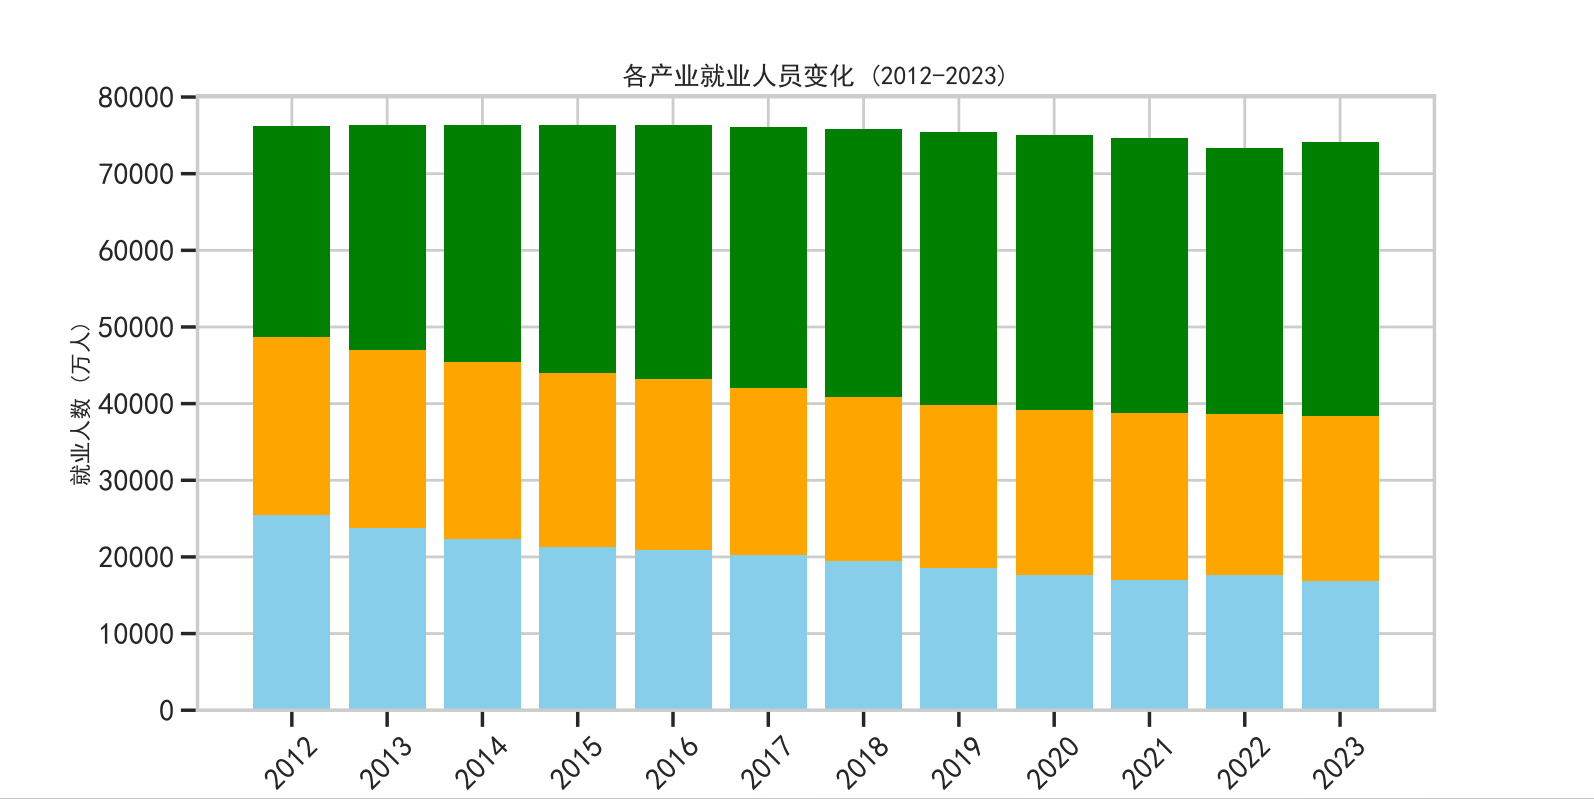
\includegraphics[width=0.7\linewidth]{figure/20各产业就业人员变化.png}
    \caption{各产业就业人员变化图}
    \label{各产业就业人员变化}
\end{figure}
从图中可以看出,随着中国经济的转型升级,劳动力市场正经历着由农业和制造业向服务业和高技术产业的结构调整。数据显示,第一产业就业人数持续下降,这与农业现代化、农村劳动力向城市转移密切相关;第二产业就业人数虽有波动,但总体呈下降趋势,反映出制造业中劳动力密集型岗位的逐步减少和产业结构的不断优化;而第三产业就业人数则稳步上升,尤其自2017年后服务业就业显著增长,预示着经济转向以高技术和服务导向为主的方向。

展望未来,随着数字经济和高技术行业的进一步发展,服务业与高端制造业将持续成为中国就业市场的主导力量。面对这种趋势,政府亟需加强对劳动力转型的支持,提升技能培训质量,促进人力资源在新兴行业中的高效配置,从而为经济高质量发展提供有力保障。
\chapter{国际影响力}
\label{chapter:impact}
习近平总书记强调,科技创新是新质生产力的核心动力,尤其在全国两会等重大契机下更显重要。在“人工智能+”背景下,科技创新不仅推动国内经济发展,还显著提升“中国制造”的国际竞争力。通过教育改革、人才培养、生产方式变革、产业升级以及优化就业结构,科技创新为国家注入新动能,激发社会活力,使中国在全球科技竞争中占据关键地位。

\section{社会变革下的政府措施}
在全球科技迅猛发展的背景下,人工智能(AI)作为新一轮产业变革的核心驱动力,正逐步成为衡量一国科技竞争力与治理能力的重要指标。基于和鲸平台的调研数据,制作出“各地区AI相关透明度措施采用情况”面积图(见图\ref{各地区AI相关透明度措施采用情况图}),直观展示了不同区域在AI透明度措施上的采纳情况。
\begin{figure}[H]
    \centering
    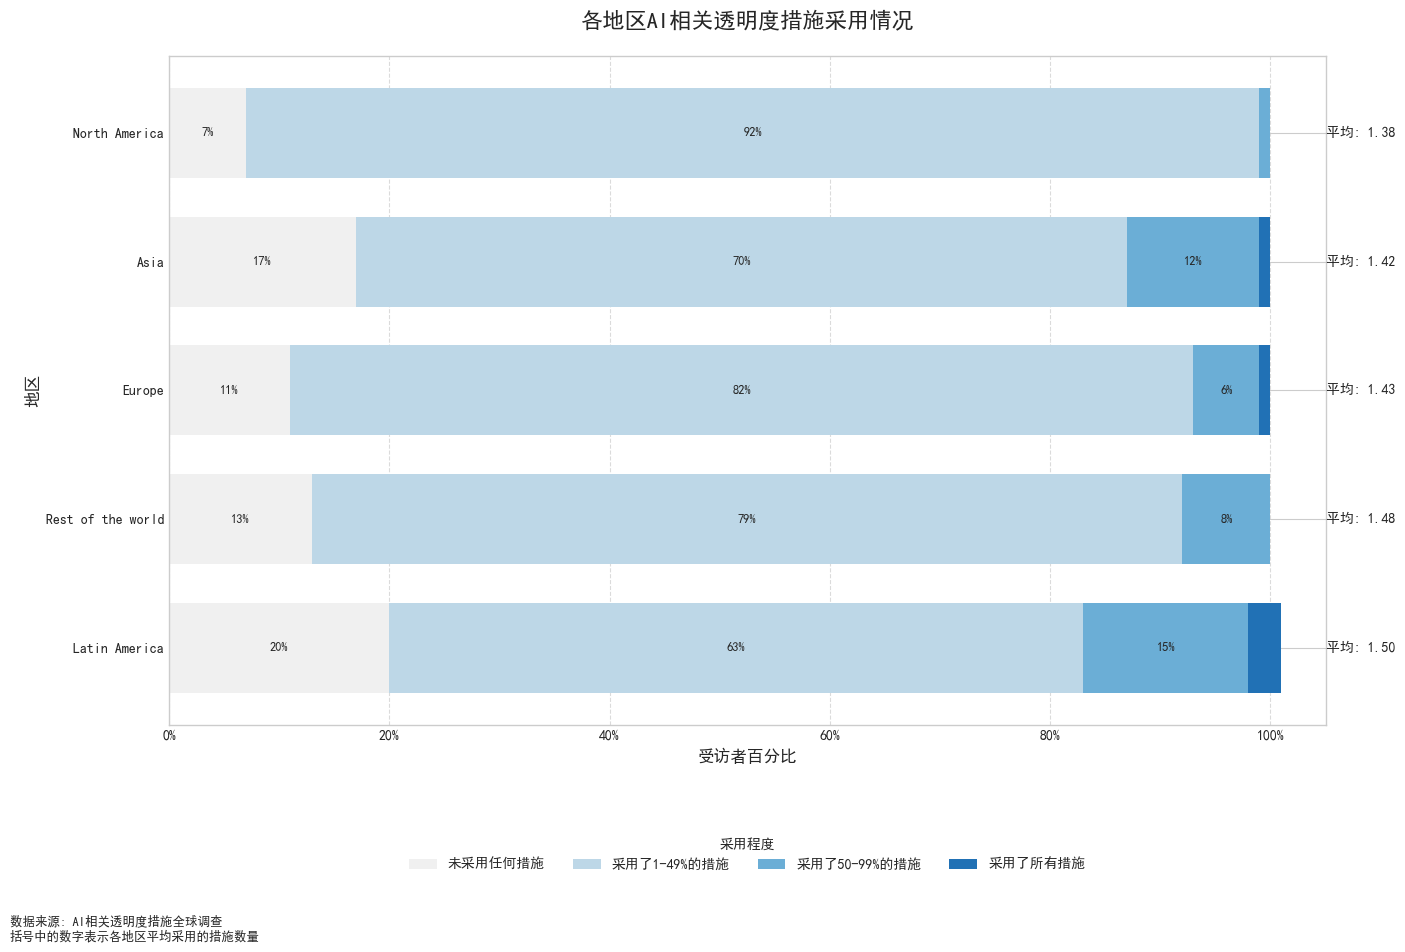
\includegraphics[width=0.7\linewidth]{figure/21各地区AI相关透明度措施采用情况图.png}
    \caption{各地区AI相关透明度措施采用情况图}
    \label{各地区AI相关透明度措施采用情况图}
\end{figure}

具体来看,北美在推广AI透明度政策上遥遥领先,高达92\%的机构已采用75\%至99\%的相关措施,另有7\%全面落实,显示出其治理框架的成熟。相比之下,亚洲70\%的机构仅执行中等级别(7\%至49\%)的措施,17\%的机构无任何行动,只有12\%的机构达到较高标准,反映出政策响应与技术实施的不均衡。欧洲则呈现两极分化:62\%的机构部分采纳,11\%的机构完全未响应,仅有6\%的机构实现全面落实,表明其制度虽具坚实基础,但执行深度仍不足。

总体而言,全球AI透明度措施推广虽已展开,但各区域在落实深度和广度上存在显著差异。北美政策体系完善但全面落实不足;亚洲与欧洲受国家发展和政策整合水平限制;而拉丁美洲及其他地区的迅速进展,则显示出新兴市场在数字治理中的潜力。

因此,我国在持续推出AI治理措施的同时,应注重提升政策执行的全面性与协调性,实现科技创新与社会责任的平衡,进而构建符合时代需求的AI治理新格局,稳步提升在全球科技生态中的话语权和引领力。\cite{butcher2023global}
\section{全球各国创新指数}
在全球科技迅猛发展的当下,创新已成为衡量一个国家综合国力与国际竞争力的关键指标。为了全面、系统地评估各国创新能力,世界知识产权组织每年发布《全球创新指数》,该指数整合了创新环境、投入、产出与成效等多个维度(见表\ref{创新指数构成表_上}和\ref{创新指数构成表_下}),已成为国际上广泛采用的重要评价工具。

根据国家统计局发布的创新指标构成数据(基准年份为2015年),以指数化形式展现各项指标的变化趋势(见图\ref{中国创新指数及分领域指数趋势图},旨在剖析我国近年来在创新领域取得的显著进步以及全球排名的稳步攀升。

\begin{figure}[H]
    \centering
    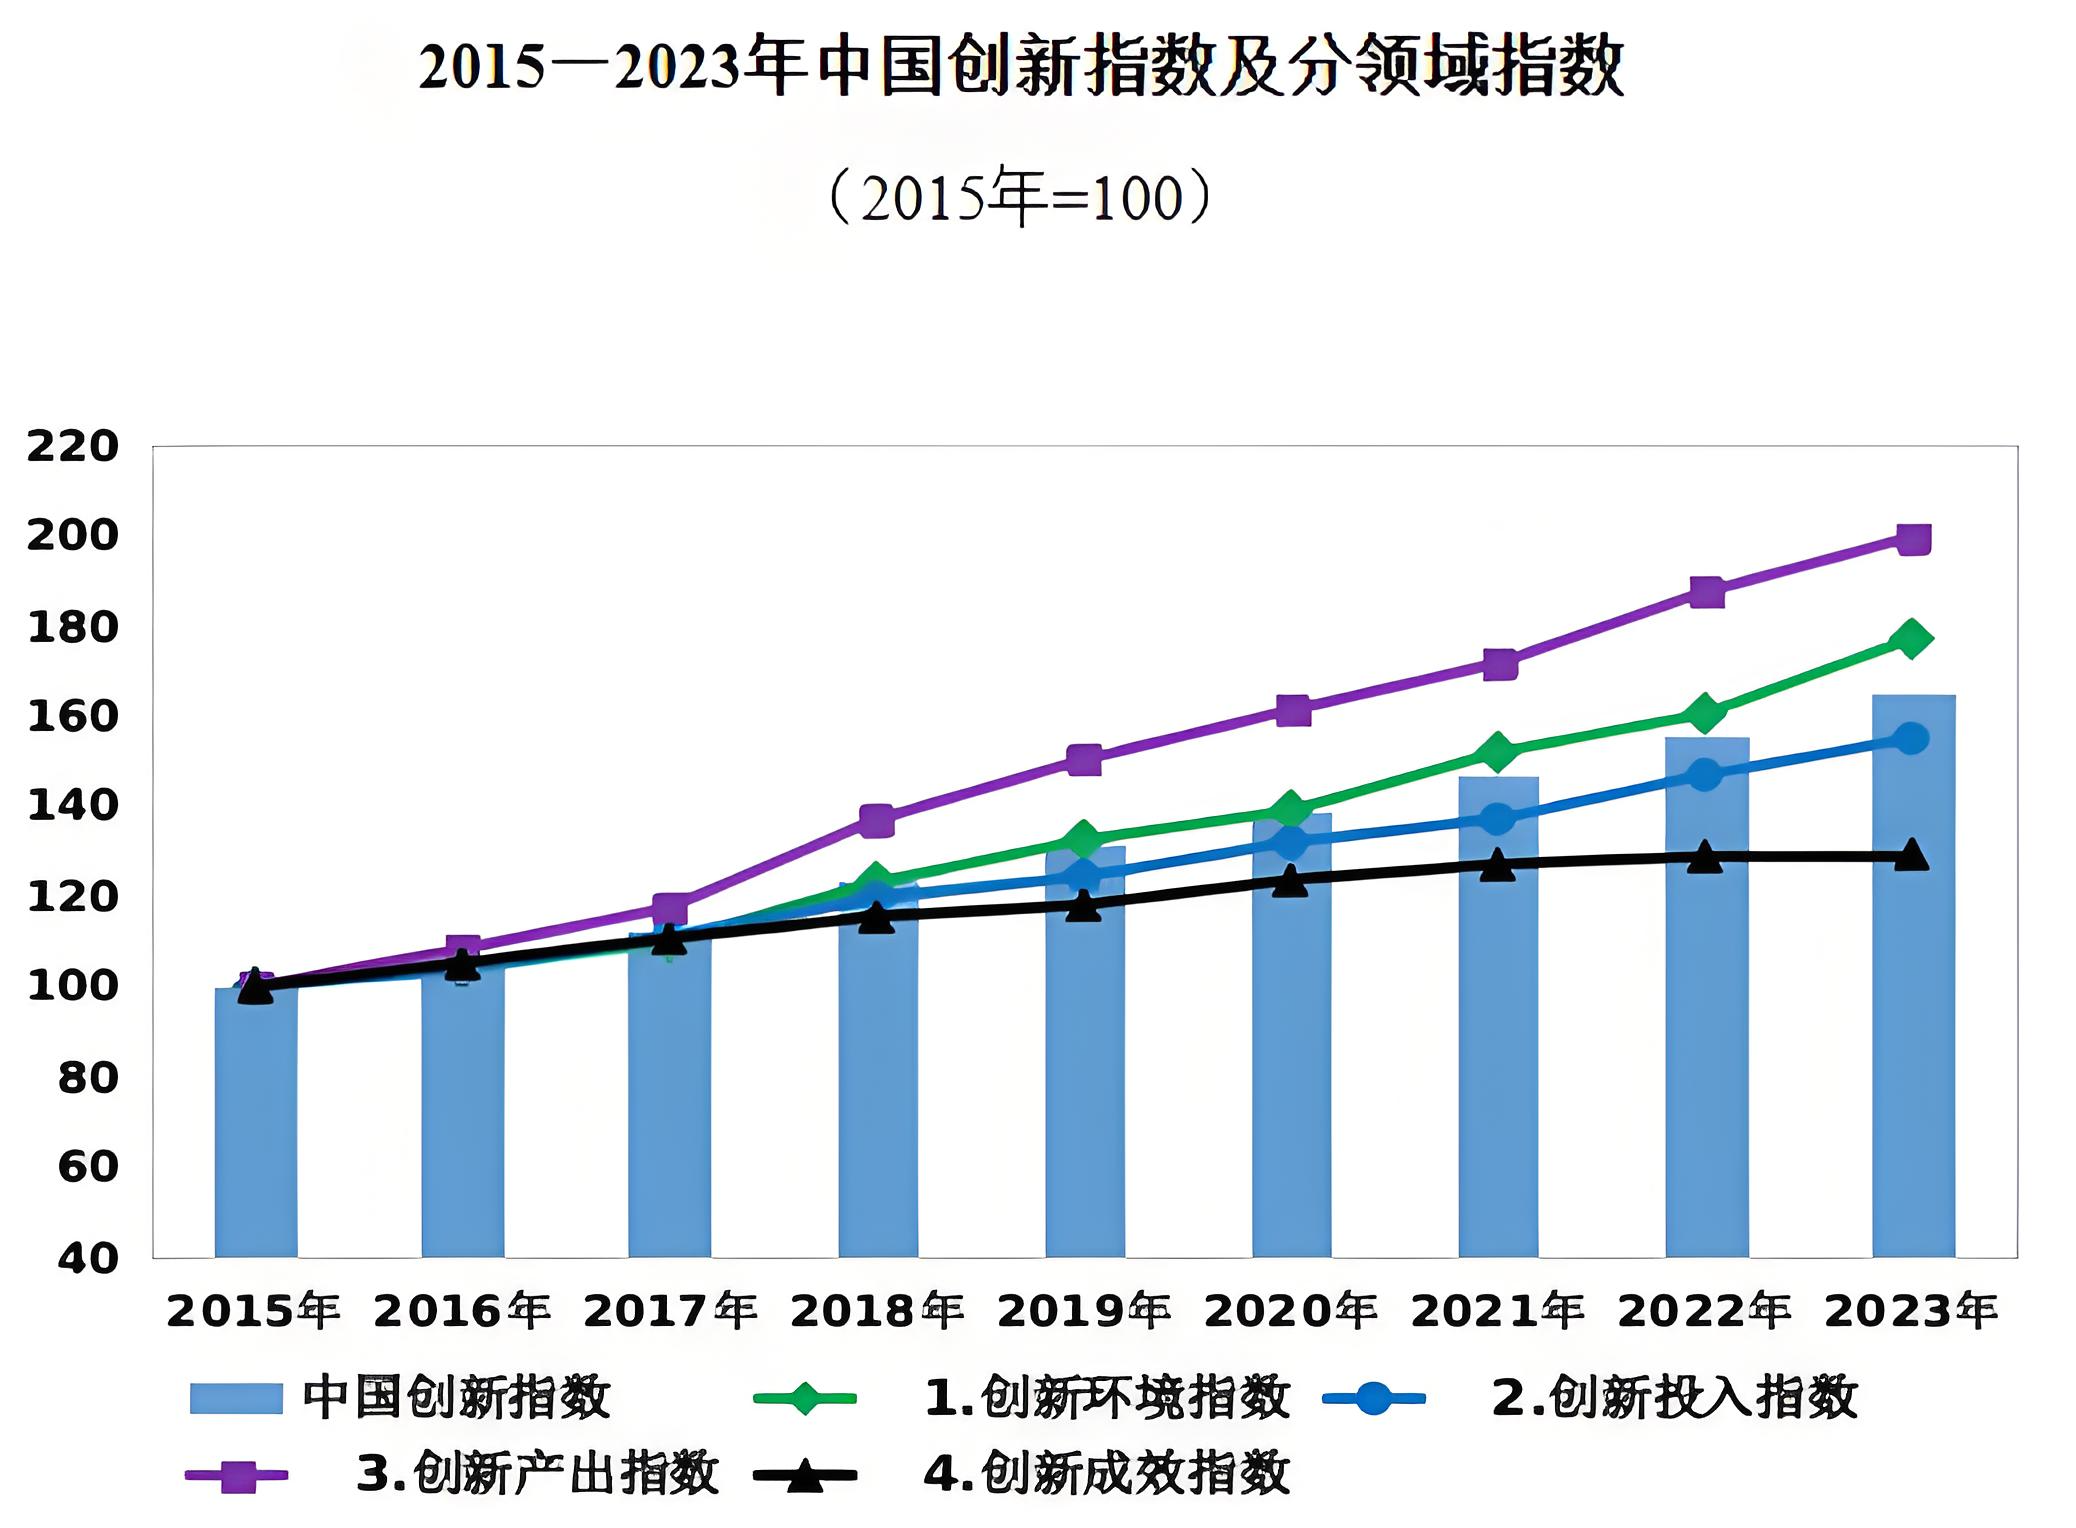
\includegraphics[width=0.7\linewidth]{figure/22中国创新指数及分领域指数趋势图.png}
    \caption{中国创新指数及分领域指数趋势图}
    \label{中国创新指数及分领域指数趋势图}
\end{figure}
自2015年设定基准(指数=100)以来,中国各项创新指标持续上扬,彰显结构优化与质量提升。总体创新指数至2023年接近180,显示出显著增长;其中,“创新产出指数”最为突出,从100迅速跃升至近210,反映科研成果显性化、技术转化效率提升及科技影响力增强;“创新投入指数”增长至近160,而“创新环境”和“创新成效指数”分别达约140与120,表明制度保障、科研氛围与教育支撑日趋完善。

尤其值得关注的是,中国在全球创新指数排名中实现历史性跃升。2024年数据显示,在132个评价国家中,中国位列第11,标志着从追赶者向引领者的转变,与长期位居前十的创新强国相比,凸显出国家科技战略的深远成效。

综上,通过量化分析及国际对比可见:中国在科技创新与自主研发能力提升上取得了实质性突破,国际竞争力显著增强。未来,若进一步深化科技体制改革、强化原始创新并推动成果转化,中国有望在更多关键领域实现从跟跑到并跑乃至领跑。建议后续补充高分辨率趋势图,以增强数据可视化和论文支撑。
\section{高技术产品出口比例}
在全球经济格局深度演变的背景下,高技术产品出口占制造业出口的比重已逐渐成为衡量一国技术发展水平和国际市场竞争力的重要指标。根据世界银行集团最新发布的数据,制作出“高技术产品出口占制造业出口的百分比”折线图(见图\ref{各国高技术产品出口占制造业出口比例趋势图}),直观展示了这一比重的变化趋势。

\begin{figure}[H]
    \centering
    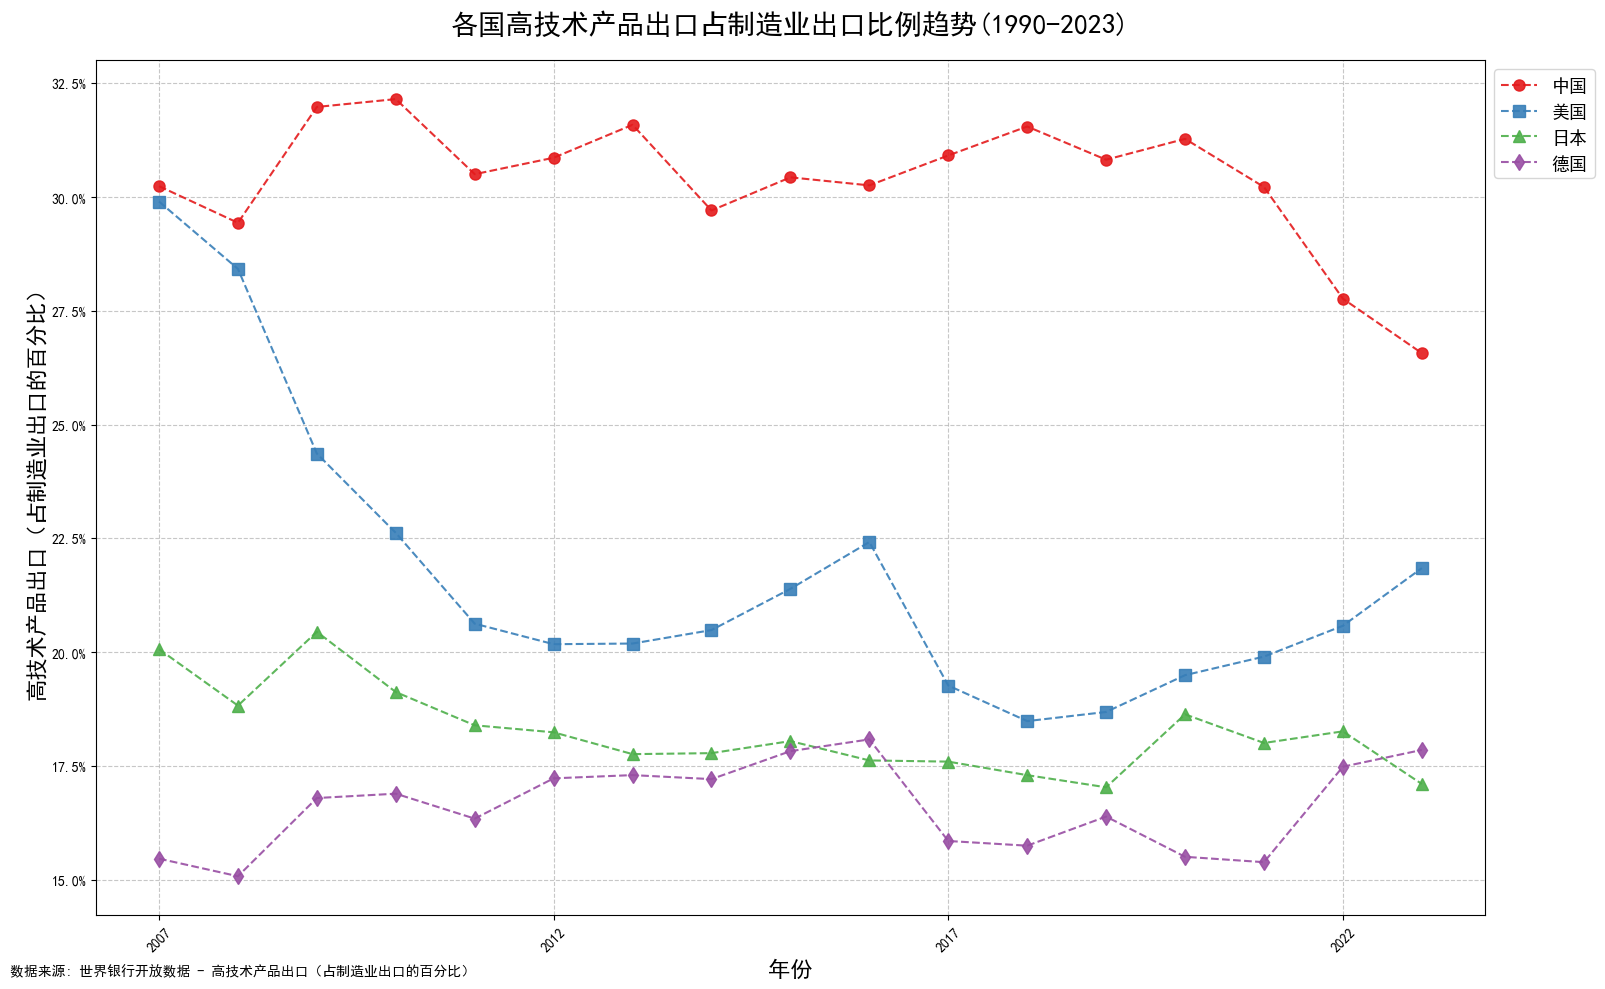
\includegraphics[width=0.7\linewidth]{figure/23各国高技术产品出口占制造业出口比例趋势图.png}
    \caption{各国高技术产品出口占制造业出口比例趋势图}
    \label{各国高技术产品出口占制造业出口比例趋势图}
\end{figure}

根据图示数据,自21世纪初以来,中国一直在该指标上保持领先,长期维持在约30\%的高位,远超美国、日本和德国。然而,自2021年以来,高技术产品出口比例明显下滑,截至2023年降至约27.5\%。同期,美国呈现温和回升,日本和德国则稳定在20\%及以下。这一变化引发了对我国高技术产业发展逻辑和外贸结构调整背景的关注,亟需多角度系统分析其内在驱动因素。

\textbf{(a) 全球竞争加剧}

近年来,越南、墨西哥及中东欧国家(如波兰、匈牙利)在全球制造业供应链中崛起,凭借低劳动力成本、优惠贸易政策与地理优势吸引大量投资。

\textbf{(b) 经济政策和产业结构调整}

近年来,中国经济政策逐步从出口导向转为内需和服务业驱动,同时推动制造业向高端和绿色转型,致使传统高技术产品在总出口中的比重下降。

\textbf{(c) 产能过剩和价格竞争}

部分高技术领域(如光伏、锂电池)存在产能过剩,导致国内竞争激烈、价格下跌,虽增强全球市场竞争力,却压缩了出口利润和比重。

\textbf{(d) 高技术产业分类和统计变化}

随着技术进步,高技术产品的定义和分类不断演变。新兴产业,如电动汽车和智能设备,可能未完全纳入传统统计范畴,导致高技术出口比重下降。

综上所述,中国高技术产品出口占比的下降,并不意味着技术能力衰退,而是多重因素作用的结果。\cite{li2021china}未来,政策制定者应结合全球市场动态优化出口结构,并通过技术创新和制度升级提升产品附加值及议价能力,从而巩固并扩大中国在全球高技术领域的战略优势。
\section{新产品投入产出}
为了全面剖析我国高技术产品出口结构的演化趋势及背后驱动逻辑,本节以“新产品投入产出”为切入点,构建“传统高技术产业出口下滑—新兴产业快速兴起—创新结构转型升级”的因果链,揭示中国在全球技术竞争中的战略调整。

基于国家统计局与和鲸平台提供的《规模以上工业企业的科技活动基本情况》数据集,绘制出2004至2023年工业企业“新产品投入产出比”柱状图(见图\ref{工业企业新产品投入产出对比}),聚焦“新三样”产业(电动载人汽车、锂离子蓄电池、太阳能电池)的迅速发展,为理解高技术出口占比下降背后的转型逻辑提供了坚实数据支撑。

\begin{figure}[H]
    \centering
    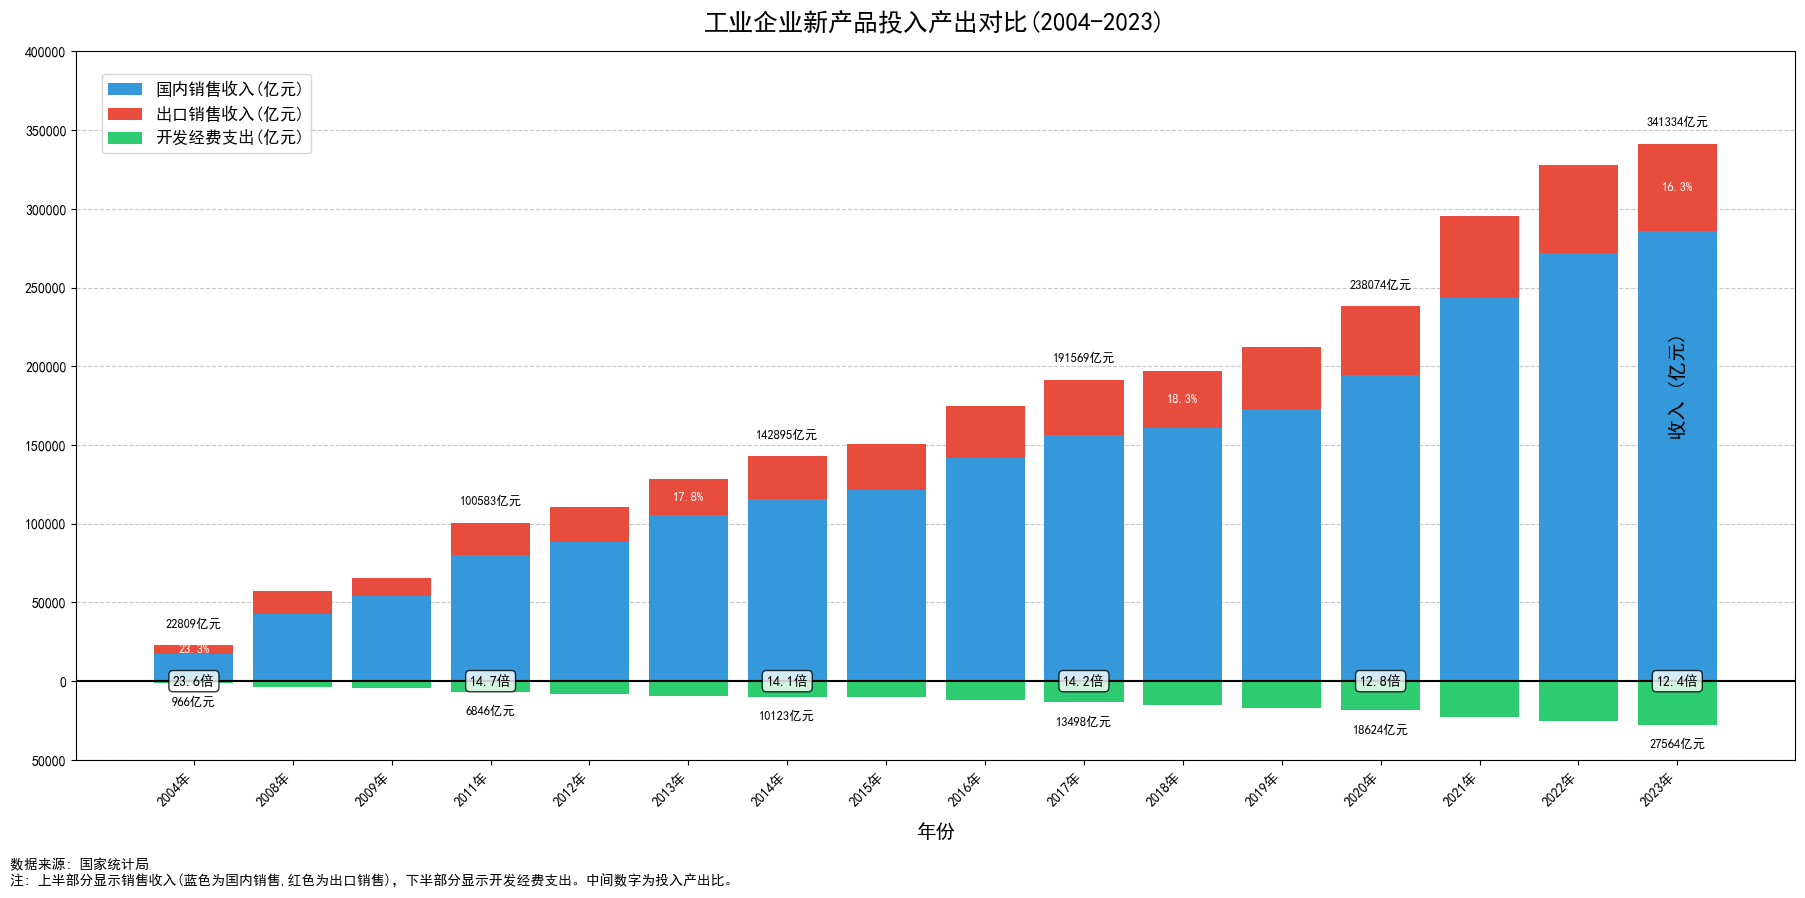
\includegraphics[width=0.7\linewidth]{figure/24工业企业新产品投入产出对比.png}
    \caption{工业企业新产品投入产出对比图}
    \label{工业企业新产品投入产出对比}
\end{figure}

自2011年以来,新产品销售收入从不足1.1万亿元飙升至2023年的34.1万亿元,增幅超30倍,年均复合增长率达20\%以上;其中出口销售收入从2015年的13.5万亿元增至2023年的27.5万亿元,接近翻倍。这表明,即便传统统计中高技术产品出口占比下降,其绝对出口额正大幅提高,中国正在从传统高技术向新兴高技术转型。

同时,2011至2023年间,研发投入与销售额的比值稳定在约12~14倍,显示新兴产业研发产出效率高、成果转化能力强。尤其2020年后,“新基建”与绿色能源政策推动电动汽车、储能电池和光伏组件等产业爆发式增长,2023年其出口增幅分别达67\%、32\%和30.5\%,虽未完全涵盖传统高技术统计,但技术含量和附加值已符合甚至超越高技术标准。

此外,工业企业研发投入于2023年达到2.8万亿元,占新产品销售额的8\%以上,形成了良性研发—产出循环,提升了产业链附加值与全球竞争力,如宁德时代、比亚迪和隆基绿能等企业在出口上持续扩大领先优势。

总体来说,高技术产品出口占比下降的背后,隐藏着新兴技术产业的崛起和结构升级,标志着中国正由传统出口向创新驱动型出口转型。\cite{zhou2021technological}
% \chapter{�����˿ڽṹ}
\label{chapter:people}

��ͼչʾ��ȫ���˿ڽṹ���긴�������ʱ仯���������ͼ�п��Եó�������Ҫ�۲��������ȣ�ȫ�򷢴���ҵ��긴�������ʽӽ����㣬����չ�й��ҵ��긴��������ͨ����1��3֮�䣬���޵Ȳ�������ҵ��긴���������򳣳���5\%�Ҳ����ϴ���Σ����й������ķ�չ�й�����ͼ����ʾΪ����ɫ���뷢������γɶԱȣ���ʾ����޴�ķ�չDZ������δ�ȶ����˿ڽṹ��������ˣ���չũ�������Ϊ��ǰ����Ҫ��չĿ��֮һ��

\begin{figure}[H]
    \centering
    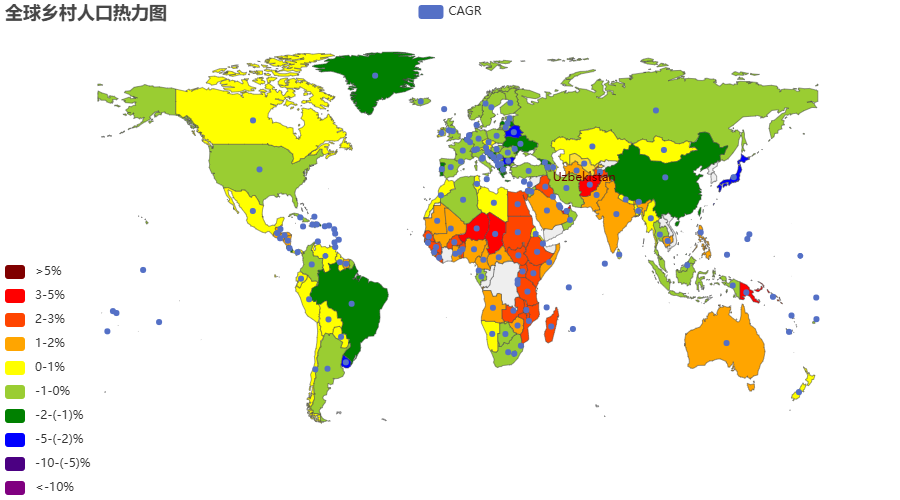
\includegraphics[width=1\linewidth]{pictures/image.png}
    \caption{ȫ������˿�����ͼ}
    \label{fig:enter-label}
\end{figure}



�Ըĸ↑���������й�ũ���������Ͷ�������д���������������һ��������������˿����仯���Ͷ�����ʧ�����⡣ΪӦ����Щ��ս����������������ս�ԣ�ּ��ͨ�����ũҵЧ�ʡ����ƻ�����ʩ�͹��������Դ�������ũ������ˮƽ���Ӷ��ٽ�ũ�徭�����ȫ�淢չ��

�����������ս�Ե�ʵʩ������˿ڽṹ�����±仯�����ǽ�����1990����2022���ÿ����������ݣ�����һϵ�б�ͼ��չʾ�й������˿ں�����˿ڵı�����

\begin{figure}[H]
    \centering
    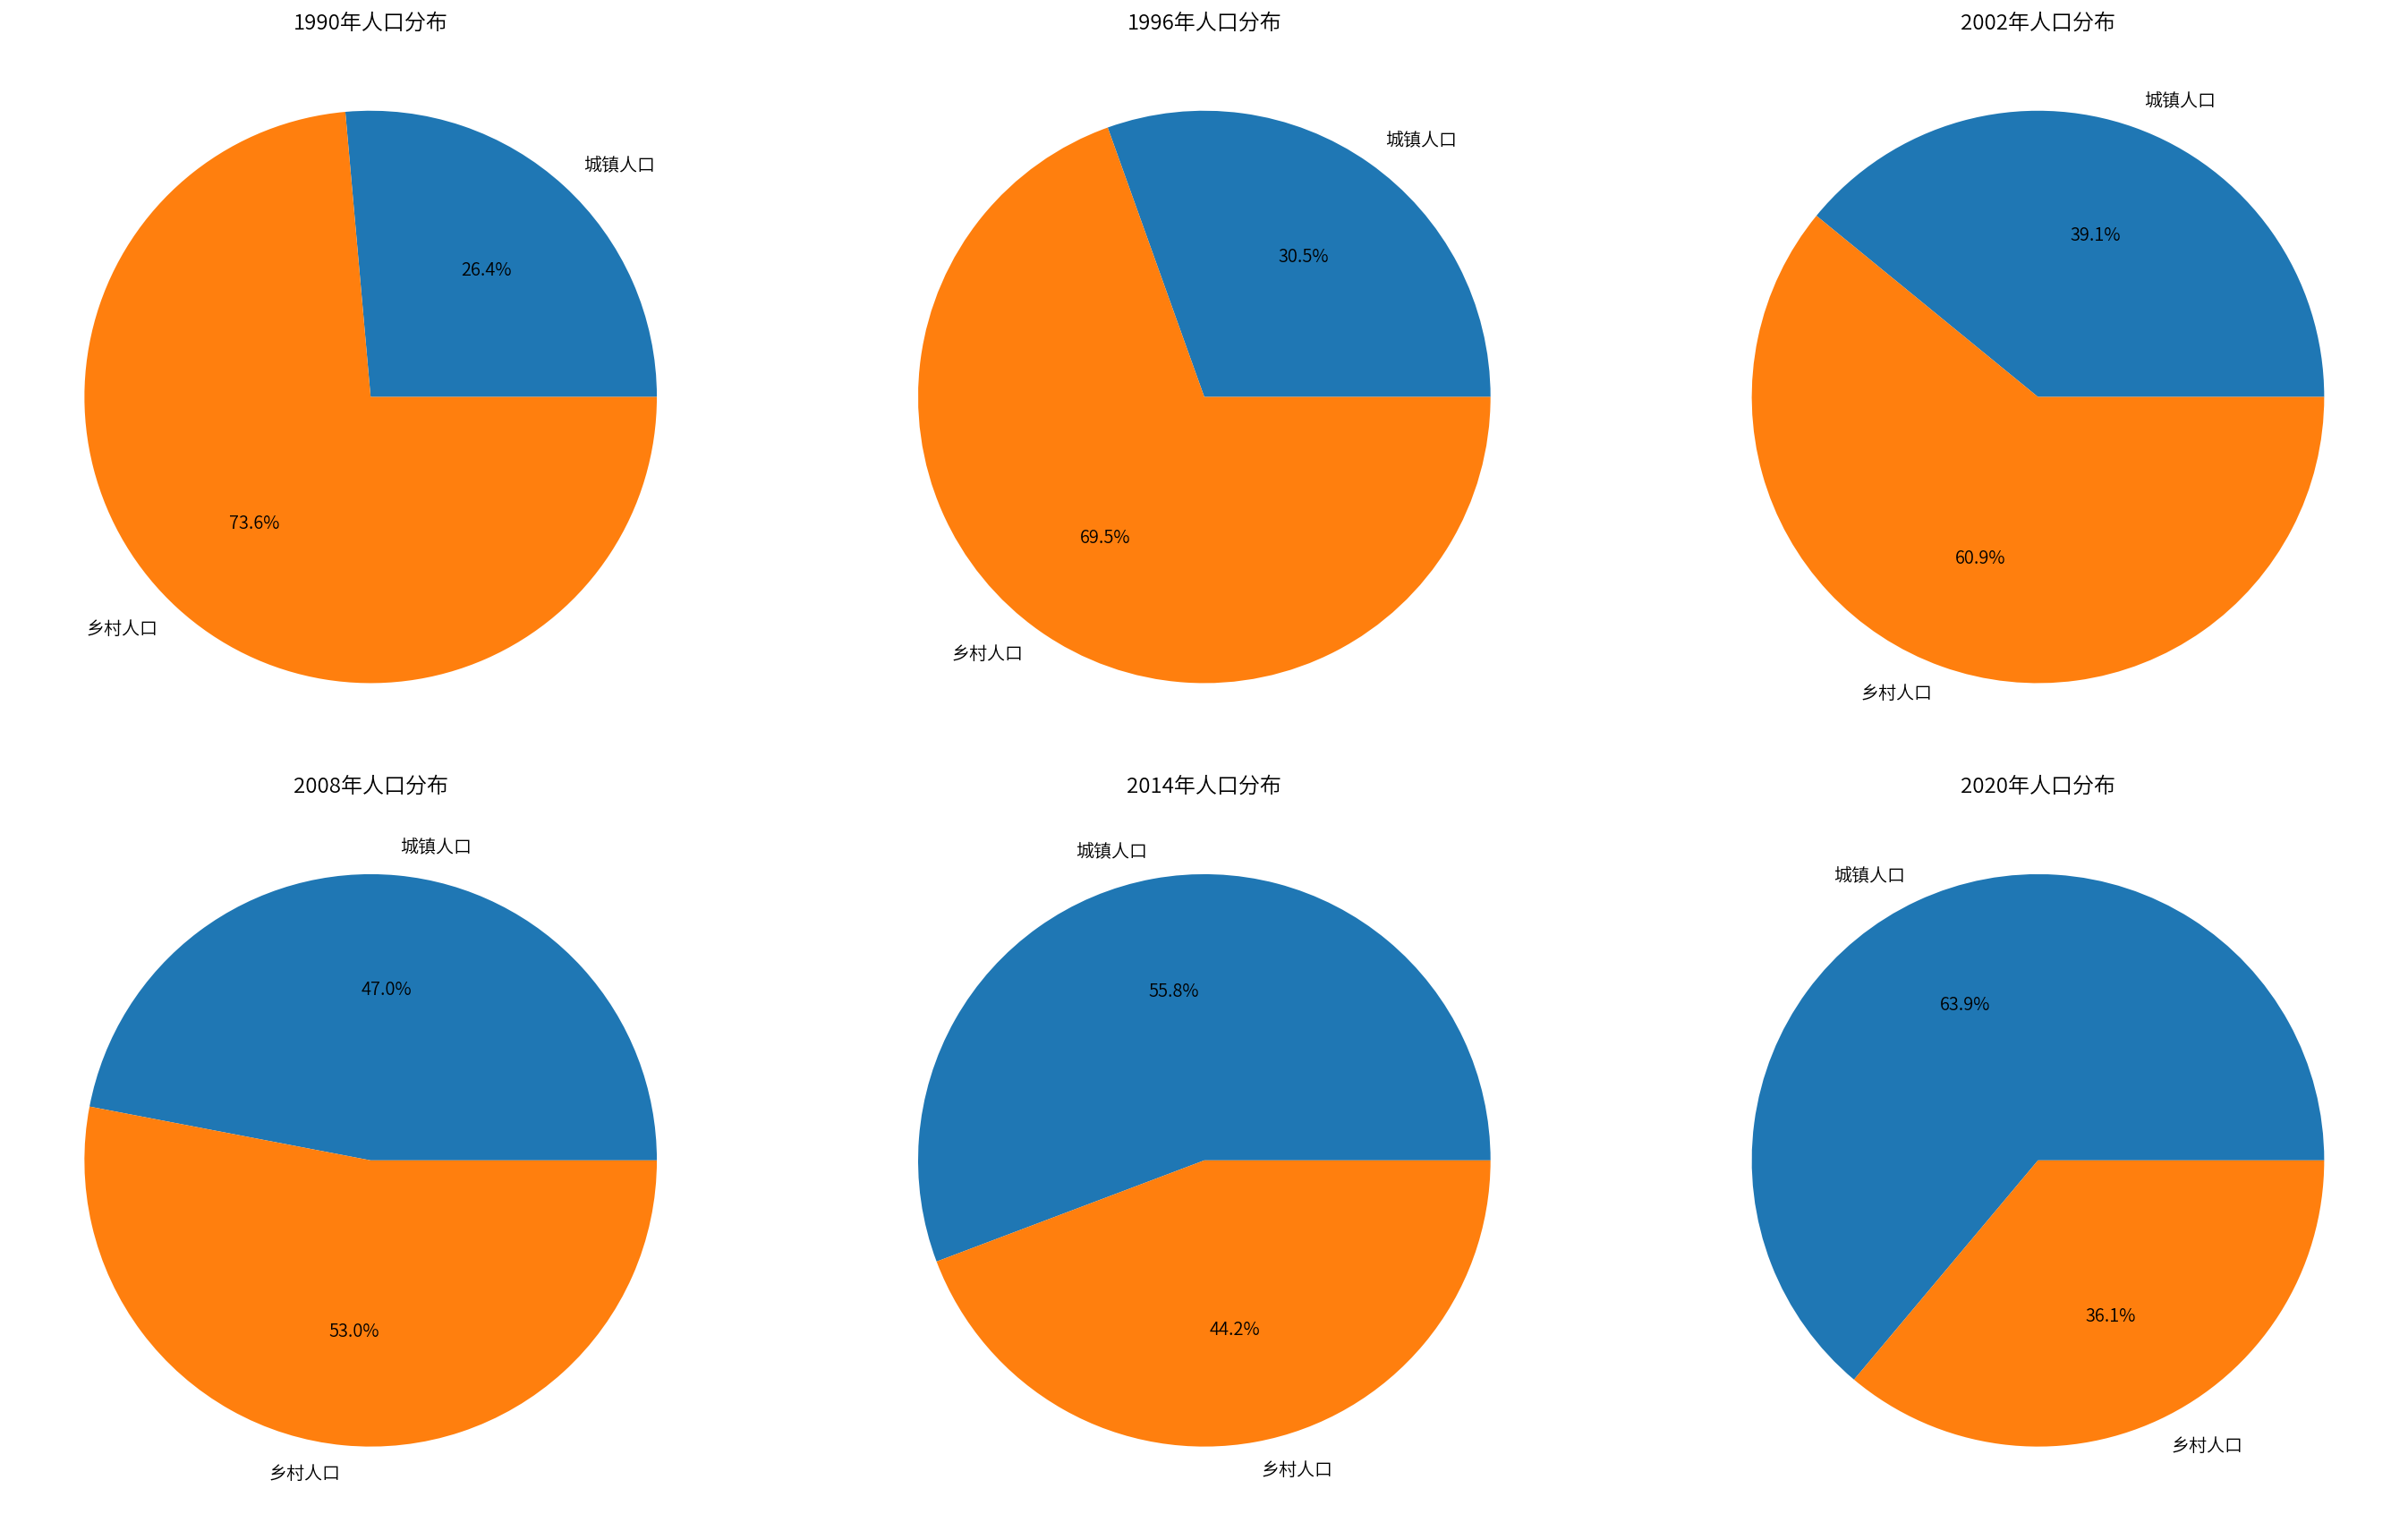
\includegraphics[width=1\linewidth]{figures/1.png}
    \caption{�����˿�ռ��ͼ}
    \label{fig:city_village_population}
\end{figure}

ͼ����ʾ�������˿�ռ������������������˿�ռ����Ӧ�������½�����һ������ĸ↑�������й����л����̵ļӿ�������ء�

% �����й����õĿ��ٷ�չ����ҵ����������Լ��������������ij������ƣ�����ũ�����������������Ѱ����õĹ�����������ᡣ��һ���Ƶ��³����˿ڱ�������������������˿ڱ�����Ӧ�������½��������˿�����������ӳ�˳���֮��ľ��ò�࣬Ҳ��ʾ��ũ������ڷ�չ���ᡢ������ʩ��������ҽ�Ƶȷ���IJ��㡣

ũ��������˿���ʧ��һ��͹����ũ�巢չ����������Ϊ�˻�����һ���ƣ������ǿũ�彨��������������ṩ����ľ�ҵ���ᣬ���ƽ�����ҽ���������Լ����ũ�������ˮƽ��Ϊũ����������������������͹�����������������˿ڵ���ʧ�ٶȣ��ٽ�����Э����չ����������������ʷ�����£��������ս��Ӧ�˶�������Ϊ���й���ɫ���������ʱ������Ҫƪ�¡�

\section{�����˿�Ԥ��}
��һ���������֣���������˿ڱ��������½������½����ٶ��ƺ��ڷŻ�����ʾ���������ٵķ����𽥼�С������ܷ�ӳ�˽������й����ƽ����緢չһ�廯��ʵʩ�������ս�Եȷ���������Ŭ����ʼ���ֳ�Ч������˿���ʧ�ٶ������Ż���

Ϊ����֤�����˿ڱ仯���ƵIJ��벢Ԥ��δ����չ�����IJ�����DLF-LSTMģ��Ԥ������������ڳ����˿ڵı仯���ơ����õ���Ԥ�����Լ�ģ�Ͷ���ʷ���ݵ�������ͨ����ͼչʾ��
\begin{figure}[H]
    \centering
    \begin{minipage}{0.5\textwidth}
        \centering
        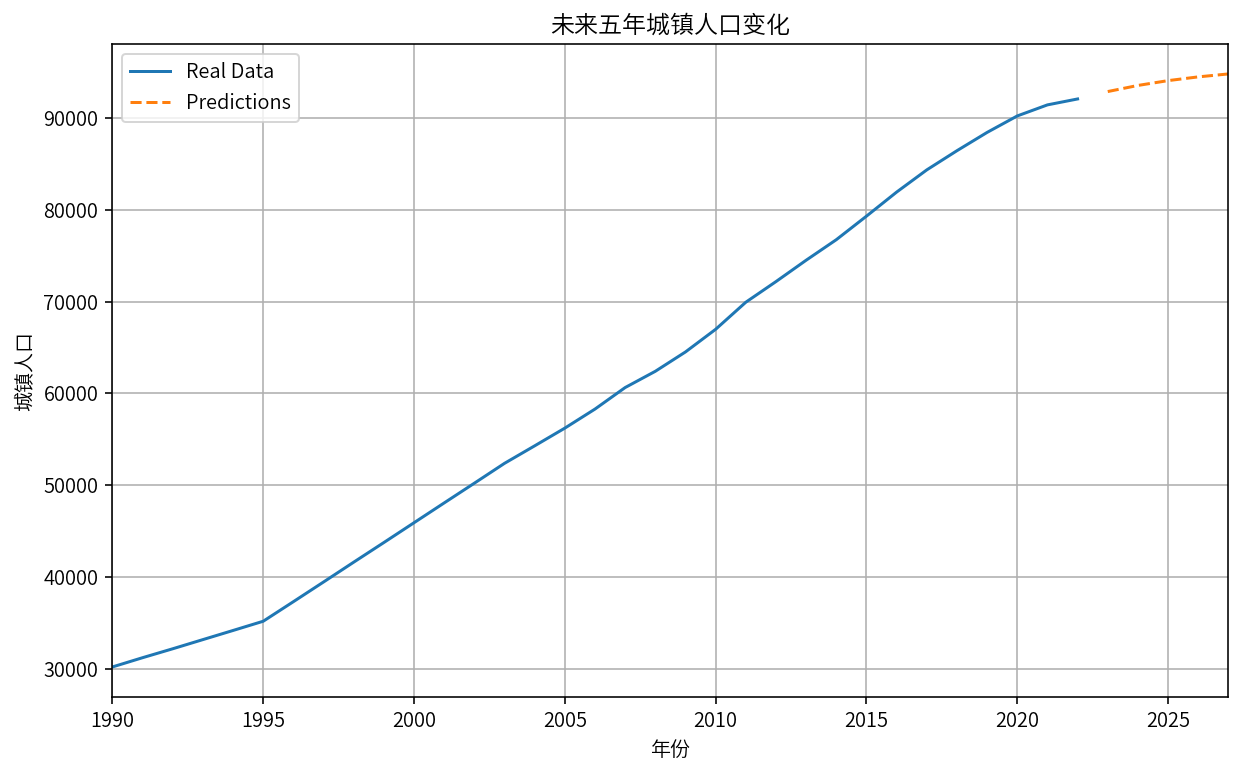
\includegraphics[width=\linewidth]{figures/2.png}
        \caption{δ����������˿ڱ仯}
        \label{fig:population-change}
    \end{minipage}\hfill
    \begin{minipage}{0.5\textwidth}
        \centering
        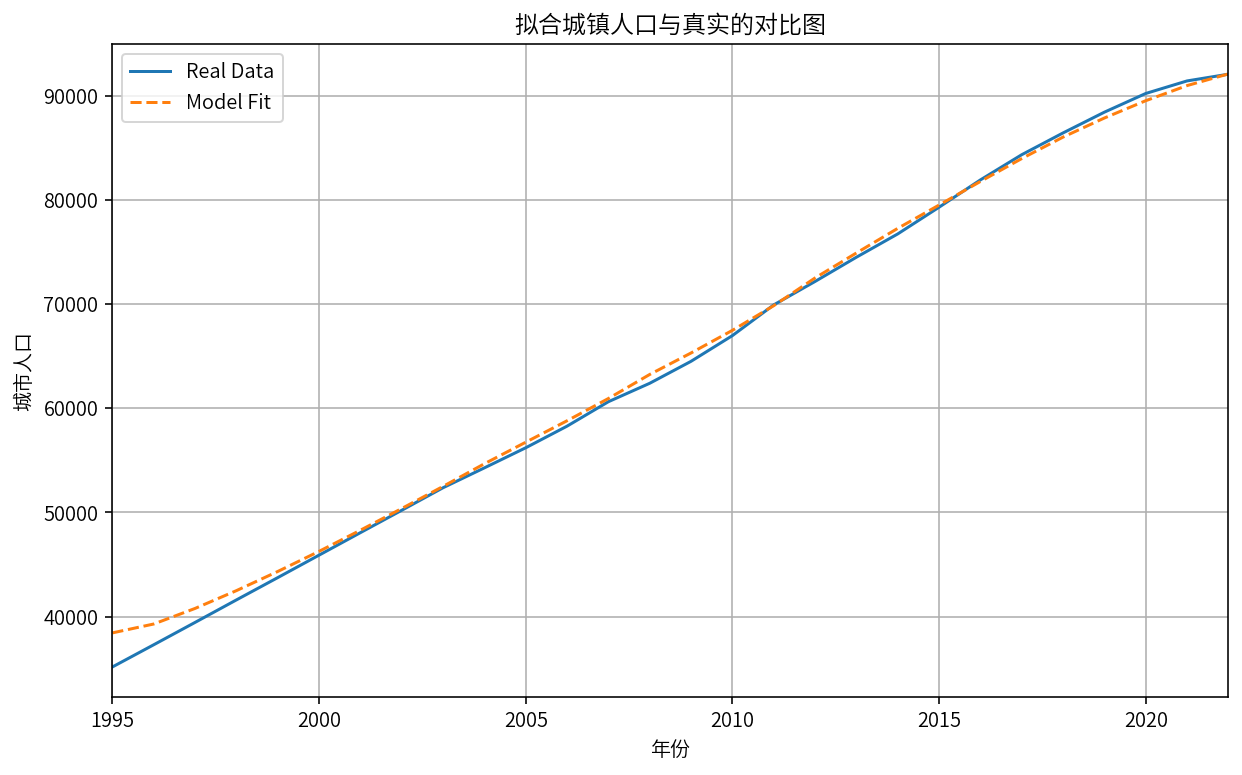
\includegraphics[width=\linewidth]{figures/3.png}
        \caption{��ϳ����˿ں���ʵ�ĶԱ�ͼ}
        \label{fig:population_fit-vs-real}
    \end{minipage}
\end{figure}

ͨ��ʱ�����е�֪�������������ƿ��ܳ��ֱ��ͣ�ֻ����΢��������

����ͬ����������ũ���˿ڵ�Ԥ�⣬���ý�����£�
\begin{figure}[H]
    \centering
    \begin{subfigure}{0.5\textwidth}
        \centering
        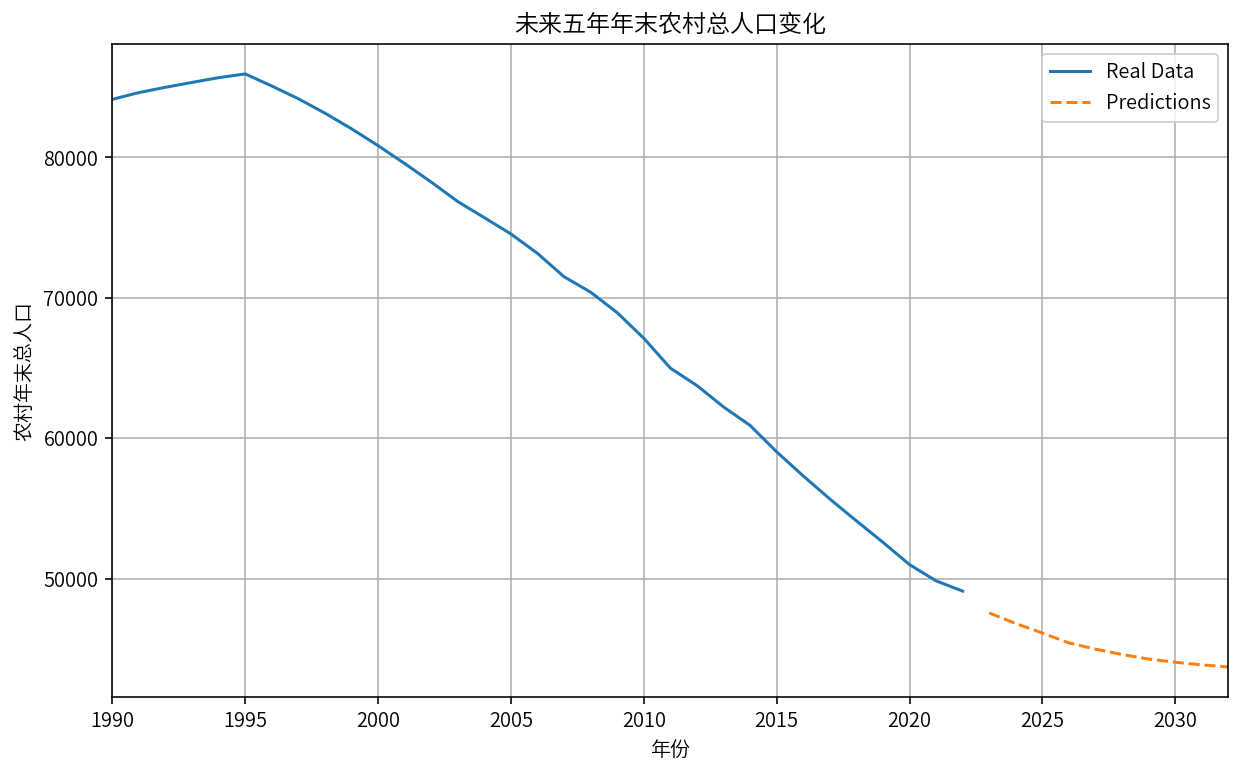
\includegraphics[width=\linewidth]{figures/35.png}
        \caption{δ������ũ���˿ڱ仯}
        \label{fig:sub1}
    \end{subfigure}%
    \begin{subfigure}{0.5\textwidth}
        \centering
        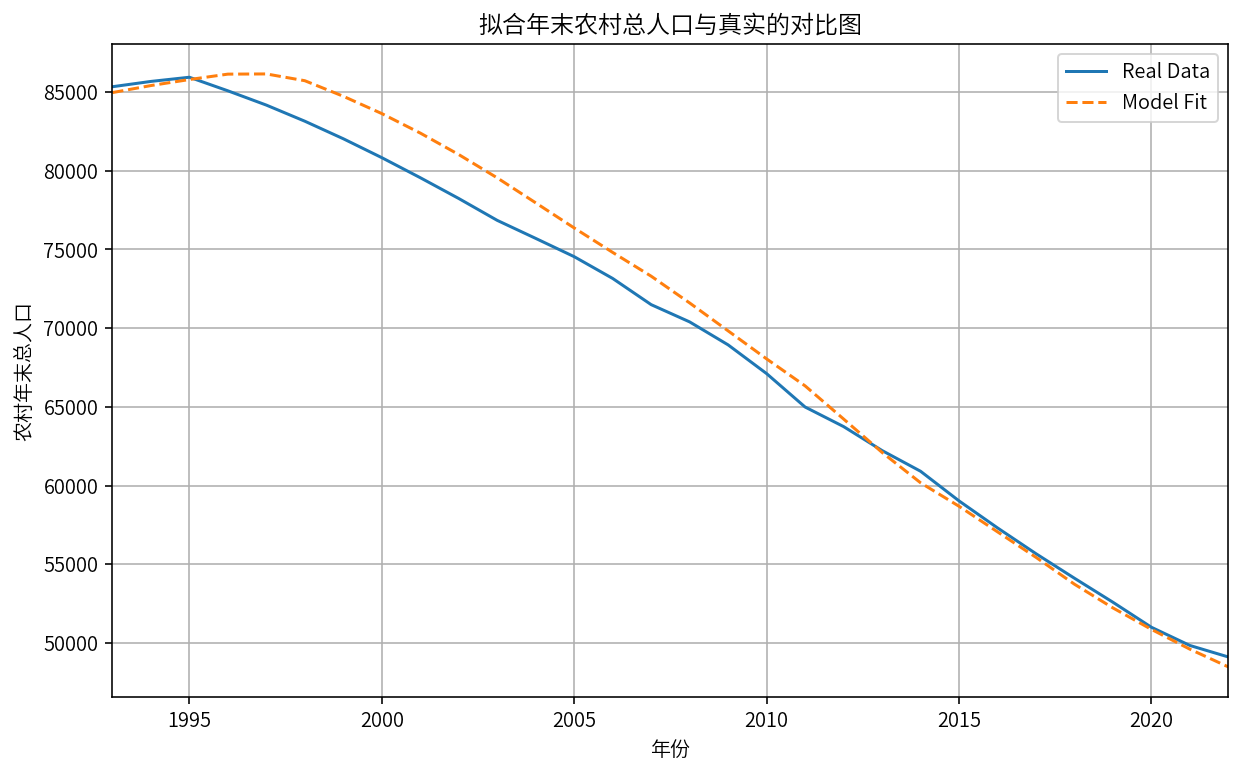
\includegraphics[width=\linewidth]{figures/36.png}
        \caption{���ũ���˿ں���ʵ�ĶԱ�ͼ}
        \label{fig:sub2}
    \end{subfigure}
    \caption{ũ���˿ڱ仯ͼ}
    \label{fig:combined}
\end{figure}

\begin{table}[h]
    \centering
    \begin{minipage}{0.48\linewidth}
        \centering
        \caption{δ�������˿�Ԥ��}
        \label{tab:urban_population_prediction}
        \begin{tabular}{cc}
        \hline
        ��� & Ԥ������˿�(����) \\
        \hline
        2023 & 92876.58 \\
        2024 & 93542.80 \\
        2025 & 94068.30 \\
        2026 & 94475.73 \\
        \hline
        \end{tabular}
    \end{minipage}\hfill
    \begin{minipage}{0.48\linewidth}
        \centering
        \caption{δ��ũ�����˿�Ԥ��}
        \label{tab:rural_population_prediction}
        \begin{tabular}{cc}
        \hline
        ��� & Ԥ��ũ�����˿�(����) \\
        \hline
        2023 & 47548.48 \\
        2024 & 46795.32 \\
        2025 & 46118.73 \\
        2026 & 45412.10 \\
        \hline
        \end{tabular}
    \end{minipage}
\end{table}



��󣬱��Ķ�ÿ��ũ���˿ڱ仯��ǰһ��ı��������˻��ܣ����Ƚ�������1�Ĵ�С������������ӽ�1ʱ��˵��ũ���˿ڵļ���������Խ�С�������������Զ��1ʱ������ζ�ű仯���Ƚϴ�

\begin{figure}[H]
    \centering
    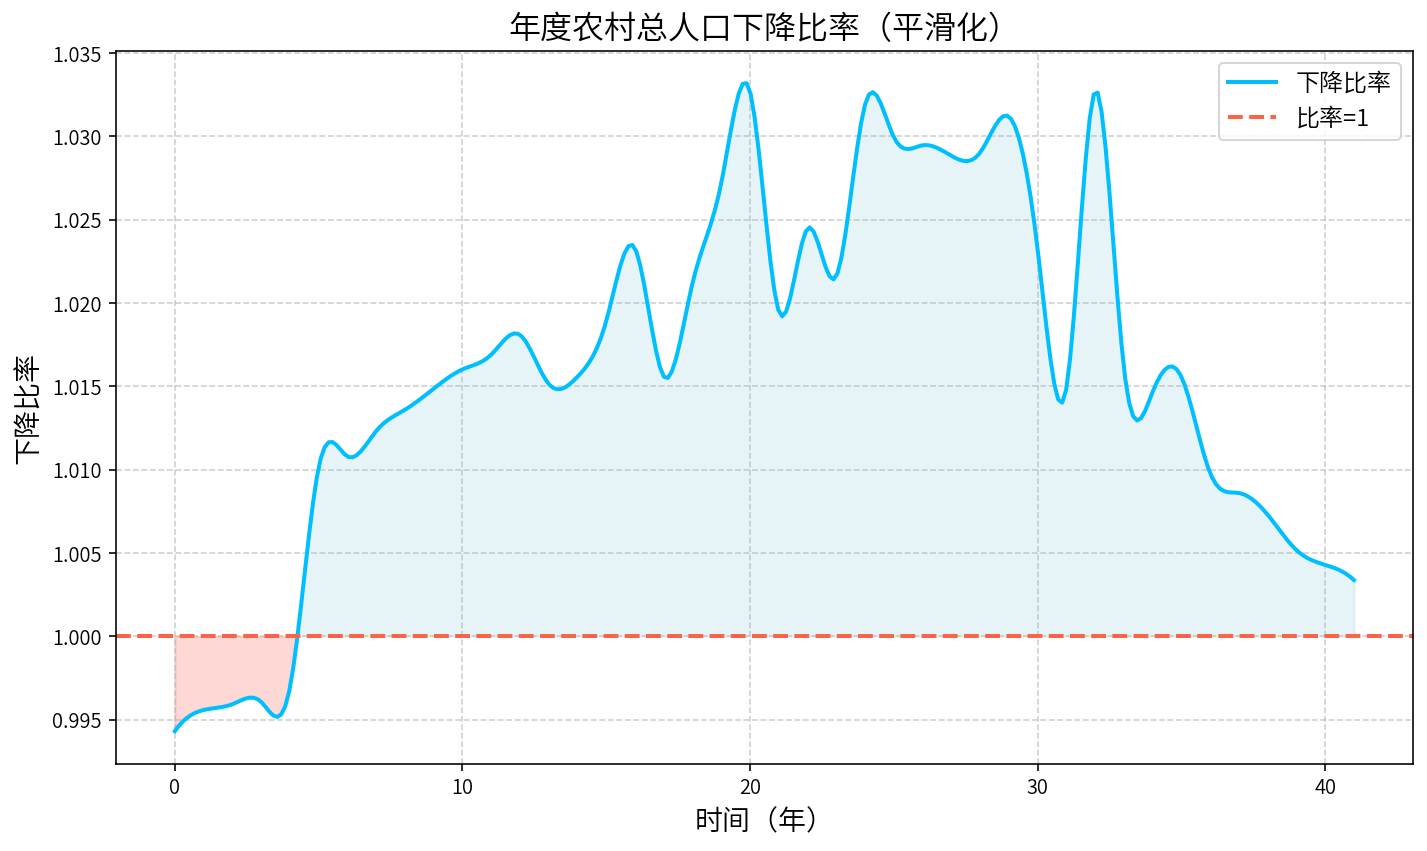
\includegraphics[width=0.65\linewidth]{figures/37.png}
    \caption{���ũ�����˿��½�����}
    \label{fig:enter-label}
\end{figure}
���ߵĽ������ʾ��ũ���˿�δ���ı仯���ƻ������ܵ�����������ߵĻ���Ӱ�죬���ֳ�������ƽ�����������������ӵ�̬�ơ��ⰵʾ����δ��һ��ʱ���ڣ�ũ��������ܻ�ӭ��һ���̶ȵ��˿ڻ�������������������ս���������Ļ��������

��һս�Բ����Ƕ��й�ũ���������̷�˼�����Ƕ�ʵ�ֳ����г��չԸ���ļᶨ׷���ڴ�ս���£�ũҵ�����ǵ�һ����ʳ����������ת��Ϊ�ִ�������Ԫ���IJ�ҵ��ϵ��ũ�岻�������Ĵ����ʣ����dz�Ϊ����������ϣ�������ء�ũ������ʱ���ı�Ե�ˣ����dz�Ϊ�����ִ������ɹ������塣

% һ���棬һЩ����ͨ������ũ������������ũҵ��ҵ�����������ɹ����������˿ڷ��紴ҵ��ع�ũҵ�����γ��˳����˿�������˫�򻥶�ģʽ����һ���棬����ũ�������ҽ�ƺ����������ĸ��ƣ�ũ����������������������ũ��������˿�����ѹ���������⣬���������ʼ���ֳ����ӻ����Ϳɳ�����չ��̬�ơ���Щ�仯��ӳ���������ս���ڵ����˿ڽṹ���ٽ�������ⷢչ����Ļ�����Ч��


\chapter{结论和展望}
\label{chapter:conclusion}
\begin{tikzpicture}[remember picture,overlay]
\node[inner sep=0pt,opacity=0.3] at (current page.center) { % Adjust the opacity here
    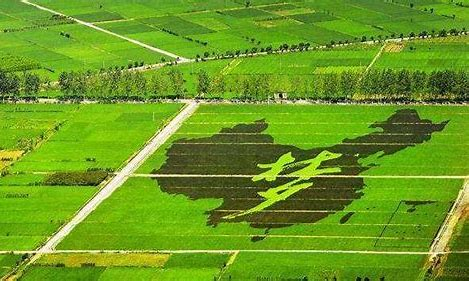
\includegraphics[width=\paperwidth,height=\paperheight]{figures/OIP-C.jpg} % Replace 'background.jpg' with your image file
};
\end{tikzpicture}

在当前的发展阶段,乡村振兴不仅关乎农业、农村和农民的未来,更是国家战略全局的重要组成部分。通过本次数据分析报告,我们得出了一写结论和展望。

必须继续大力稳固粮食安全,这是国家的根本。正如习主席所强调的,“要把中国人的饭碗牢牢端在自己手中”,我们将继续保持粮食生产的稳定性,确保每一粒粮食都能得到妥善利用。

数字农业的发展是提升农业现代化水平的关键。尽管当前数字农业渗透率尚显不足,但我们将加强数字技术在农业中的应用,推动农业生产方式的转变,如《2020年中国农村数字发展报告》所述,通过数字化转型,实现农业的智能化、精准化。

对于偏远地区,推进基础设施建设是实现乡村振兴的前提。我们将加大投资力度,改善交通、水利、电力等基础设施,为乡村发展提供坚实的物质基础。

乡村旅游业的发展是乡村振兴的一大亮点。我们将依托各地的自然风光和文化遗产,打造特色旅游产品,吸引更多游客,带动乡村经济的多元化发展。

优化产业结构,促进私营企业和个体户的发展,是提高农村经济效益的重要途径。我们将制定更多优惠政策,支持乡村产业的创新和升级,增强乡村经济的内生动力。

为促进人口回流,我们将继续完善公共服务,提高农村居民的生活质量,使乡村成为人们向往的美好家园。如习主席所言,“要让农民在乡村振兴中有更多获得感”,我们将努力实现城乡居民的共同富裕。

乡村振兴战略的实施,需要我们在保障粮食安全、推进数字农业、加强基础设施建设、发展乡村旅游业、优化产业结构和促进人口回流等多个方面下功夫。我们将以实事求是的态度,贯彻落实两会精神和三农政策,为实现乡村全面振兴而不懈努力!





\setcounter{biburlnumpenalty}{7000}
\setcounter{biburllcpenalty}{7000}
\setcounter{biburlucpenalty}{7000}
\printbibliography[heading=bibintoc,title=参考文献]

%\newpage
\section{Appendix}
\begin{lstlisting}[language=python,caption={两会数据爬虫}]
# 两会是现在的热门话题,从两会讨论的话题中,来看乡村发展的必要性
import requests
from bs4 import BeautifulSoup
headers = {
    "User-Agent": "Mozilla/5.0 (Windows NT 10.0; Win64; x64) AppleWebKit/537.36 (KHTML, like Gecko) Chrome/121.0.0.0 Safari/537.36 Edg/121.0.0.0"
}
texts = [] # 提取两会文本
for i in range(0,9):
    if(i!=0) :
        url = f"https://www.gov.cn/zhuanti/2024qglh/2024nzfgzbg/home_{i}.htm"
    else:
        url = "https://www.gov.cn/zhuanti/2024qglh/2024nzfgzbg/home.htm"
    response = requests.get(url,headers=headers)
    response.encoding="utf-8"
    content = response.text
    soup = BeautifulSoup(content,"html.parser")
    # 定位到特定的<div>容器
    container = soup.find('div', class_="list list_1 list_2")
    # 在这个容器内查找所有的<a>标签
    links = container.find_all('a')
    # 提取并打印所有<a>标签的文本内容
    for link in links:
        texts.append(link.get_text())
print(texts)
# 筛选出包含 '乡' 字的文本项
texts_containing_char = [text for text in texts if '农' in text or '乡' in text  or '村' in text or '城' in text or '绿' in text]

# 打印结果
for text in texts_containing_char:
    print(text)
    ## 输出高清图像
%config InlineBackend.figure_format = 'retina'
%matplotlib inline
import numpy as np
import matplotlib.pyplot as plt
from wordcloud import WordCloud
 
text = "Love"
 
x, y = np.ogrid[:300, :300]
 
mask = (x - 150) ** 2 + (y - 150) ** 2 > 130 ** 2
mask = 255 * mask.astype(int)
wc = WordCloud(background_color="white", repeat=True, mask=mask)
wc.generate(text)
 
plt.axis("off")
plt.imshow(wc, interpolation="bilinear")
plt.show()
import numpy as np
import matplotlib.pyplot as plt
from wordcloud import WordCloud
 
# 合并文本数据
text = """
从两会看中国经济:打好乡村全面振兴漂亮仗
推动城乡融合和区域协调发展 大力优化经济布局
扎实推进乡村全面振兴
推动城乡融合和区域协调发展
推动传统产业高端化、智能化、绿色化转型!
政府工作报告中的绿色低碳发展
今年要把促进农业转移人口市民化放在突出位置来抓
加强生态文明建设,推进绿色低碳发展
推动城乡融合和区域协调发展,大力优化经济布局
坚持不懈抓好“三农”工作,扎实推进乡村全面振兴
"""
 
x, y = np.ogrid[:300, :300]
 
mask = (x - 150) ** 2 + (y - 150) ** 2 > 130 ** 2
mask = 255 * mask.astype(int)
 
 
wc = WordCloud(background_color="white", repeat=True, mask=mask)
wc.generate(text)
 
plt.axis("off")
plt.imshow(wc, interpolation="bilinear")
plt.show()
from wordcloud import WordCloud
import matplotlib.pyplot as plt

# Your text data
text = """
从两会看中国经济:打好乡村全面振兴漂亮仗
推动城乡融合和区域协调发展 大力优化经济布局
扎实推进乡村全面振兴
推动城乡融合和区域协调发展
推动传统产业高端化、智能化、绿色化转型!
政府工作报告中的绿色低碳发展
今年要把促进农业转移人口市民化放在突出位置来抓
加强生态文明建设,推进绿色低碳发展
推动城乡融合和区域协调发展,大力优化经济布局
坚持不懈抓好“三农”工作,扎实推进乡村全面振兴
"""

# Generating the word cloud
wordcloud = WordCloud(
    font_path='/home/mw/project/SourceHanSansSC-Regular.ttf',
    background_color='white',
    collocations=False,
    max_words=50,
    max_font_size=100,
    min_font_size=10,
    scale=10
).generate(text)

# Displaying the word cloud image
plt.figure(figsize=(10, 5))
plt.imshow(wordcloud, interpolation='bilinear')
plt.axis('off')
plt.show()
from wordcloud import WordCloud
import matplotlib.pyplot as plt

# 合并文本数据
text = """
从两会看中国经济:打好乡村全面振兴漂亮仗
推动城乡融合和区域协调发展 大力优化经济布局
扎实推进乡村全面振兴
推动城乡融合和区域协调发展
今年要把促进农业转移人口市民化放在突出位置来抓
推动城乡融合和区域协调发展,大力优化经济布局
坚持不懈抓好“三农”工作,扎实推进乡村全面振兴
"""

# 生成词云,增加scale参数
wordcloud = WordCloud(
    font_path='/home/mw/project/SourceHanSansSC-Regular.ttf',
    width=800,
    height=400,
    background_color='white',
    collocations=False,
    max_words=50,
    max_font_size=100,
    min_font_size=10,
    scale=2  # 增加输出图像的分辨率
).generate(text)

# 显示词云图像
plt.figure(figsize=(10, 5))
plt.imshow(wordcloud, interpolation='bilinear')
plt.axis('off')
plt.show()
import jieba.posseg as pseg
\end{lstlisting}
\begin{lstlisting}[language=python,caption={全国乡村产业发展规划}]
file_path = '/home/mw/input/planning5088/《全国乡村产业发展规划(2020-2025年)》全文.txt'

with open(file_path, 'r', encoding='utf-8') as file:
    article_content = file.read()
    ## 输出高清图像
%config InlineBackend.figure_format = 'retina'
%matplotlib inline
import re
cleaned_content = re.sub(r'[^\w\s]', '', article_content) 
cleaned_content = re.sub(r'\d', '', cleaned_content)     
cleaned_content = cleaned_content.replace('\n', '')
import jieba as jb
from wordcloud import WordCloud
import matplotlib.pyplot as plt
words_to_remove = ['乡村', '农村', '农业', '产业', '发展', '振兴','的','等','和']
for word in words_to_remove:
    cleaned_content = cleaned_content.replace(word, '')
    cleaned_content = jb.lcut(cleaned_content)
cleaned_content  =  '/'.join(cleaned_content)
wordcloud = WordCloud(collocations=False,font_path='/home/mw/project/SourceHanSansSC-Regular.ttf', width=3000, height=2000, margin=2,background_color='white').generate(cleaned_content)
# 显示图片 
plt.imshow(wordcloud) 
plt.axis('off')
plt.show()

\end{lstlisting}
\begin{lstlisting}[language=python,caption={主要农作物播种面积和产品产量数据
}]
import pandas as pd
file_path = '/home/mw/input/develop6699/主要农作物播种面积和产品产量数据.csv'
data = pd.read_csv(file_path,encoding='GBK')
# 按照时间为列做整理
data = data.set_index('指标').T
data.reset_index(inplace=True)
data.rename(columns={'index': '年份'}, inplace=True)
data.head()
# 改为数值方便统计
data['年份'] = data['年份'].str.replace('年', '')
data = data.sort_values(by='年份')
data.head()
## 输出高清图像
%config InlineBackend.figure_format = 'retina'
%matplotlib inline
import seaborn as sns
import matplotlib.pyplot as plt
selected_columns = ['年份', '小麦产量(万吨)', '稻谷产量(万吨)', '大豆产量(万吨)', '玉米产量(万吨)']
heatmap_data = data[selected_columns].set_index('年份')
heatmap_data = heatmap_data.astype('float').transpose()
step = len(filtered_heatmap_data.columns) // 5  
years_to_display = filtered_heatmap_data.columns[::step]
plt.figure(figsize=(10, 6))
for crop in filtered_heatmap_data.index:
    plt.plot(filtered_heatmap_data.columns, filtered_heatmap_data.loc[crop], marker='o', label=crop)

plt.xticks(years_to_display, [int(year) for year in years_to_display])

plt.title('主要粮食产量变化')
plt.xlabel('年份')
plt.ylabel('产量')
plt.legend()
plt.grid(True)
plt.show()
# 输出每种农作物随时间的变化
# 每条折线为不同类型农作物的播种面积
import matplotlib.pyplot as plt

indicators = data.columns[1:] 
indicator_groups = [indicators[i:i + 10] for i in range(0, len(indicators), 10)]
for i, group in enumerate(indicator_groups):
    plt.figure(figsize=(15, 8))
    for indicator in group:
        plt.plot(data['年份'], data[indicator], label=indicator)

    plt.title(f'农作物播种面积和产量指标:图 {i+1}')
    plt.xlabel('年份')
    plt.ylabel('数值')
    plt.xticks(rotation=45)
    plt.legend()
    plt.grid(True)
    plt.tight_layout()
    plt.show()
    import matplotlib.pyplot as plt


selected_indicators = transposed_data.columns[1:10] 

plt.figure(figsize=(15, 8))

for year in transposed_data['年份']:
    plt.plot(selected_indicators, transposed_data[transposed_data['年份'] == year].iloc[0, 1:10], label=year)

plt.xlabel('指标')
plt.ylabel('面积/产量')
plt.title('1990-2022年各指标的年度变化')
plt.xticks(rotation=45)
plt.legend(loc='upper left', ncol=2, title='年份')
plt.grid(True)
plt.show()

# 输出每种农作物随时间的变化
# 每条折线为时间线

import matplotlib.pyplot as plt


indicator_groups = [data.columns[1:][i:i + 10] for i in range(0, len(data.columns[1:]), 10)]


for i, group in enumerate(indicator_groups):
    plt.figure(figsize=(15, 8))


    for year in data['年份']:
        plt.plot(group, data[data['年份'] == year].iloc[0][group], label=year)

    plt.xlabel('指标')
    plt.ylabel('面积/产量')
    plt.title(f'1990-2022年各指标的年度变化 - 图 {i+1}')
    plt.xticks(rotation=45, ha='right')
    plt.legend(loc='upper left', ncol=2, title='年份')
    plt.grid(True)
    plt.tight_layout()
    plt.show()
    import numpy as np

# 准备玫瑰图的数据
categories = data['年份']
values = data['农作物总播种面积(千公顷)']
N = len(categories)

# 计算每个类别的角度
angles = [n / float(N) * 2 * np.pi for n in range(N)]
values = np.concatenate((values, [values[0]]))  # 闭合图形
angles += angles[:1]

# 计算平均值以标准化数据
mean_value = data['农作物总播种面积(千公顷)'].mean()

# 标准化值(与平均值的差异)
normalized_values = data['农作物总播种面积(千公顷)'] - mean_value

plt.figure(figsize=(12, 8))
ax = plt.subplot(111, polar=True)

# 绘制标准化的值
ax.plot(angles, list(normalized_values) + [normalized_values[0]])
ax.fill(angles, list(normalized_values) + [normalized_values[0]], 'b', alpha=0.1)

plt.xticks(angles[:-1], categories, color='black', size=10)
plt.title('1990-2022年农作物总播种面积的变化(相对于平均值) - 玫瑰图')
plt.show()


\end{lstlisting}\begin{lstlisting}[language=python,caption={十四五规划可视化}]
import pandas as pd
# 读取数据时使用GBK
file_path = '/home/mw/input/1458039/十四五计划.csv'
data = pd.read_csv(file_path,encoding='GBK')
data.head()
## 输出高清图像
%config InlineBackend.figure_format = 'retina'
%matplotlib inline
import pandas as pd
import matplotlib.pyplot as plt
# 为了排版美观,将数据进行翻转
# 转置数据框,使得各个指标成为行,年份成为列
data_transposed = data.set_index('年份').T
data_transposed.columns = data_transposed.columns.map(str)  # 将年份的列名转换为字符串

# 对每个指标的数据进行归一化处理,确保其和为1(或100%)
data_normalized = data_transposed.div(data_transposed.sum(axis=1), axis=0)

# 绘制堆叠条形图,纵坐标为各种指标,每个条形图内部展示2020年和2025年数据的百分比
ax = data_normalized.plot(kind='barh', stacked=True, figsize=(10, 8))

# 设置图例
ax.legend(title='年份', loc='center left', bbox_to_anchor=(1, 0.5))

# 添加标签和标题
ax.set_xlabel('百分比')
ax.set_ylabel('指标')
ax.set_title('各指标在2020年与2025年的百分比堆叠条形图')

# 显示图表
plt.tight_layout()
plt.show()
\end{lstlisting}
\begin{lstlisting}[language=python,caption={主要贡献}]
import pandas as pd
file_path = '/home/mw/input/develop6699/全国农业主要科技贡献相关指标.csv'
data = pd.read_csv(file_path)
print(data)
## 图像显示中文的问题
import matplotlib

import seaborn as sns

## 输出高清图像
%config InlineBackend.figure_format = 'retina'
%matplotlib inline
import matplotlib.pyplot as plt
# Creating the time series plot without using sns.set
plt.figure(figsize=(15, 8))
sns.lineplot(x='时间', y='数值', hue='品类', data=filtered_data, marker='o')

# Adding title and labels
plt.title('全国农业主要科技贡献相关指标的时间序列图')
plt.xlabel('年份')
plt.ylabel('数值 (%)')
plt.xticks(rotation=45)
# plt.legend(title='品类')

# Show the plot
plt.show()
import numpy as np

# Preparing data for the heatmap
# Pivot the data to get years as columns and categories as rows
heatmap_data = data.pivot_table(values='数值', index='品类', columns='时间', aggfunc=np.mean)

# Creating the heatmap
plt.figure(figsize=(12, 8))
sns.heatmap(heatmap_data, annot=True, cmap='YlGnBu', linewidths=.5)

# Adding title and labels
plt.title('全国农业主要科技贡献相关指标的热力图')
plt.xlabel('年份')
plt.ylabel('品类')

# Show the plot
plt.show()
\end{lstlisting}
\begin{lstlisting}[language=python,caption={数字农业渗透}]
## 输出高清图像
%config InlineBackend.figure_format = 'retina'
%matplotlib inline
import pandas as pd

# 读取数据时使用GBK
file_path = '/home/mw/input/shentou8131/数字农业渗透率.csv'
data = pd.read_csv(file_path,encoding='GBK')

print(data)
## 输出高清图像
%config InlineBackend.figure_format = 'retina'
%matplotlib inline
import matplotlib.pyplot as plt
import numpy as np
# 将百分数改为浮点数值
data['渗透率'] = data['年份'].str.rstrip('%').astype('float')

# 计算同比变化率
data['变化率'] = data['渗透率'].pct_change() * 100

# 计算每年的渗透率差异
data['年度差值'] = data['渗透率'].diff()

# 创建一个包含渗透率的条形图
fig, ax1 = plt.subplots()

color = 'tab:blue'
ax1.set_xlabel('年份')
ax1.set_ylabel('数字化渗透率 (%)', color=color)
ax1.bar(data['农业数字化渗透率'], data['渗透率'], color=color, alpha=0.6)
ax1.tick_params(axis='y', labelcolor=color)

# 创建带有年度差异的折线图
ax2 = ax1.twinx()  
color = 'tab:red'
ax2.set_ylabel('年度差值 (%)', color=color)  
ax2.plot(data['农业数字化渗透率'], data['年度差值'], color=color, marker='o', linestyle='-', linewidth=2)
ax2.tick_params(axis='y', labelcolor=color)

fig.tight_layout()  
plt.title('农业数字化渗透率及其年度差值')
plt.show()
# 更正列标头及其值
data.columns = ['年份', '农业数字化渗透率']
data['农业数字化渗透率'] = data['农业数字化渗透率'].str.rstrip('%').astype(float) / 100
data
import torch
import torch.nn as nn
import numpy as np
import matplotlib.pyplot as plt
from sklearn.preprocessing import MinMaxScaler
## 封装成一个函数,便于调用(用于处理字典)

def predict(data, train_window, future_pred, label, epochs,lr):

    # 转换为 numpy 数组
    data_np = np.array(data[label]).reshape(-1, 1)

    # 数据归一化
    scaler = MinMaxScaler(feature_range=(-1, 1))
    data_normalized = scaler.fit_transform(data_np)

    # 转换为 PyTorch tensors
    data_normalized = torch.FloatTensor(data_normalized).view(-1)

    # 创建数据集
    def create_inout_sequences(input_data, tw):
        inout_seq = []
        L = len(input_data)
        for i in range(L-tw):
            train_seq = input_data[i:i+tw]
            train_label = input_data[i+tw:i+tw+1]
            inout_seq.append((train_seq, train_label))
        return inout_seq

    train_inout_seq = create_inout_sequences(data_normalized, train_window)

    # 定义 LSTM 模型
    class LSTM(nn.Module):
        def __init__(self, input_size=1, hidden_layer_size=100, output_size=1):
            super().__init__()
            self.hidden_layer_size = hidden_layer_size

            self.lstm = nn.LSTM(input_size, hidden_layer_size)

            self.linear = nn.Linear(hidden_layer_size, output_size)

            self.hidden_cell = (torch.zeros(1, 1, self.hidden_layer_size),
                                torch.zeros(1, 1, self.hidden_layer_size))

        def forward(self, input_seq):
            lstm_out, self.hidden_cell = self.lstm(input_seq.view(len(input_seq), 1, -1), self.hidden_cell)
            predictions = self.linear(lstm_out.view(len(input_seq), -1))
            return predictions[-1]

    # 实例化模型
    model = LSTM()
    loss_function = nn.MSELoss()
    optimizer = torch.optim.Adam(model.parameters(), lr)

    # 训练模型
    # epochs = 25

    loss_values = [] 

    for epoch in range(epochs):
        for seq, labels in train_inout_seq:
            optimizer.zero_grad()
            model.hidden_cell = (torch.zeros(1, 1, model.hidden_layer_size),
                                torch.zeros(1, 1, model.hidden_layer_size))

            y_pred = model(seq)

            single_loss = loss_function(y_pred, labels)
            single_loss.backward()
            optimizer.step()

        if epoch % 5 == 1:
            loss_values.append(single_loss.item())  # Store the loss value
            print(f'epoch: {epoch:3} loss: {single_loss.item():10.8f}')

    print(f'epoch: {epoch:3} loss: {single_loss.item():10.10f}')





    # 使用matplotlib绘制图形
    plt.figure(figsize=(10, 6))
    plt.plot(loss_values, marker='o', linestyle='-', color='b')
    plt.title('Loss Reduction Over Epochs')
    plt.xlabel('Epoch')
    plt.ylabel('Loss')
    plt.grid(True)
    plt.show()


    # 使用模型对整个数据集进行预测以创建拟合与真实数据对比图
    # 为预测做准备
    test_inputs = data_normalized[-train_window:].tolist()

    # 预测未来
    model.eval()
    for i in range(future_pred):
        seq = torch.FloatTensor(test_inputs[-train_window:])
        with torch.no_grad():
            model.hidden_cell = (torch.zeros(1, 1, model.hidden_layer_size),
                                torch.zeros(1, 1, model.hidden_layer_size))
            test_inputs.append(model(seq).item())
    # 将预测数据转换回原始规模
    actual_predictions = scaler.inverse_transform(np.array(test_inputs[train_window:]).reshape(-1, 1))
    predicted_years = np.arange(data["年份"].iloc[-1] + 1 - train_window, data["年份"].iloc[-1] + 1 + future_pred)


    # # 输出预测的未来私营企业乡村就业人员数值
    # predicted_years = np.arange(data["年份"][-1] + 1 - train_window, data["年份"][-1] + 1 + future_pred)
    for year, population in zip(predicted_years, actual_predictions):
        print(f"年份: {year}, 预测{label}(万人): {population[0]:.2f}")

    # 绘制图表
    plt.figure(figsize=(10, 6))
    plt.title(f'未来{label}变化预测')
    plt.xlabel('年份')
    plt.ylabel(f'{label}')
    plt.grid(True)
    plt.autoscale(axis='x', tight=True)
    
    # 绘制实际数据
    plt.plot(data["年份"], data[label], label='Real Data')
    
    # 绘制预测数据
    plt.plot(predicted_years, np.concatenate([data[label][-train_window:], actual_predictions.ravel()]), label='Predictions', linestyle='--')
    
    plt.legend()
    plt.show()
    # # 将预测数据转换回原始规模
    # actual_predictions = scaler.inverse_transform(np.array(test_inputs[train_window:]).reshape(-1, 1))

    # # 输出预测的未来私营企业乡村就业人员数值
    # predicted_years = np.arange(data["年份"][-1] + 1, data["年份"][-1] + 1 + future_pred)
    # for year, population in zip(predicted_years, actual_predictions):
    #     print(f"年份: {year}, 预测{label}(万人): {population[0]:.2f}")

    # # 绘制图表
    # plt.figure(figsize=(10, 6))
    # plt.title(f'未来{label}变化预测')
    # plt.xlabel('年份')
    # plt.ylabel(f'{label}')
    # plt.grid(True)
    # plt.autoscale(axis='x', tight=True)
    # plt.plot(data["年份"], data[label], label='Real Data')
    # plt.plot(predicted_years, actual_predictions, label='Predictions', linestyle='--')
    # plt.legend()
    # plt.show()
    ## 封装成一个函数,便于调用(用于处理字典)

def predict(data, train_window, future_pred, label, epochs,lr):

  
    # 转换为 numpy 数组
    data_np = np.array(data[label]).reshape(-1, 1)

    # 数据归一化
    scaler = MinMaxScaler(feature_range=(-1, 1))
    data_normalized = scaler.fit_transform(data_np)

    # 转换为 PyTorch tensors
    data_normalized = torch.FloatTensor(data_normalized).view(-1)

    # 创建数据集
    def create_inout_sequences(input_data, tw):
        inout_seq = []
        L = len(input_data)
        for i in range(L-tw):
            train_seq = input_data[i:i+tw]
            train_label = input_data[i+tw:i+tw+1]
            inout_seq.append((train_seq, train_label))
        return inout_seq

    train_inout_seq = create_inout_sequences(data_normalized, train_window)

    # 定义 LSTM 模型
    class LSTM(nn.Module):
        def __init__(self, input_size=1, hidden_layer_size=100, output_size=1):
            super().__init__()
            self.hidden_layer_size = hidden_layer_size

            self.lstm = nn.LSTM(input_size, hidden_layer_size)

            self.linear = nn.Linear(hidden_layer_size, output_size)

            self.hidden_cell = (torch.zeros(1, 1, self.hidden_layer_size),
                                torch.zeros(1, 1, self.hidden_layer_size))

        def forward(self, input_seq):
            lstm_out, self.hidden_cell = self.lstm(input_seq.view(len(input_seq), 1, -1), self.hidden_cell)
            predictions = self.linear(lstm_out.view(len(input_seq), -1))
            return predictions[-1]

    # 实例化模型
    model = LSTM()
    loss_function = nn.MSELoss()
    optimizer = torch.optim.Adam(model.parameters(), lr)

    # 训练模型
    # epochs = 25

    loss_values = [] 

    for epoch in range(epochs):
        for seq, labels in train_inout_seq:
            optimizer.zero_grad()
            model.hidden_cell = (torch.zeros(1, 1, model.hidden_layer_size),
                                torch.zeros(1, 1, model.hidden_layer_size))

            y_pred = model(seq)

            single_loss = loss_function(y_pred, labels)
            single_loss.backward()
            optimizer.step()

        if epoch % 5 == 1:
            loss_values.append(single_loss.item())  # Store the loss value
            print(f'epoch: {epoch:3} loss: {single_loss.item():10.8f}')

    print(f'epoch: {epoch:3} loss: {single_loss.item():10.10f}')

    # 使用matplotlib绘制图形
    plt.figure(figsize=(10, 6))
    plt.plot(loss_values, marker='o', linestyle='-', color='b')
    plt.title('Loss 变化图')
    plt.xlabel('Epoch')
    plt.ylabel('Loss')
    plt.grid(True)
    plt.show()


    # 使用模型对整个数据集进行预测以创建拟合与真实数据对比图
    # 为预测做准备
    test_inputs = data_normalized[-train_window:].tolist()

    # 预测未来
    model.eval()
    for i in range(future_pred):
        seq = torch.FloatTensor(test_inputs[-train_window:])
        with torch.no_grad():
            model.hidden_cell = (torch.zeros(1, 1, model.hidden_layer_size),
                                torch.zeros(1, 1, model.hidden_layer_size))
            test_inputs.append(model(seq).item())
    # 将预测数据转换回原始规模
    actual_predictions = scaler.inverse_transform(np.array(test_inputs[train_window:]).reshape(-1, 1))
    predicted_years = np.arange(data["年份"].iloc[-1] + 1 - train_window, data["年份"].iloc[-1] + 1 + future_pred)


    # # 输出预测的未来私营企业乡村就业人员数值
    # predicted_years = np.arange(data["年份"][-1] + 1 - train_window, data["年份"][-1] + 1 + future_pred)
    for year, population in zip(predicted_years, actual_predictions):
        print(f"年份: {year}, 预测{label}(万人): {population[0]:.2f}")

    # 绘制图表
    plt.figure(figsize=(10, 6))
    plt.title(f'未来{label}变化预测')
    plt.xlabel('年份')
    plt.ylabel(f'{label}')
    plt.grid(True)
    plt.autoscale(axis='x', tight=True)
    
    # 绘制实际数据
    plt.plot(data["年份"], data[label], label='Real Data')
    
    # 绘制预测数据
    plt.plot(predicted_years, np.concatenate([data[label][-train_window:], actual_predictions.ravel()]), label='Predictions', linestyle='--')
    
    plt.legend()
    plt.show()
    # # 将预测数据转换回原始规模
    # actual_predictions = scaler.inverse_transform(np.array(test_inputs[train_window:]).reshape(-1, 1))

    # # 输出预测的未来私营企业乡村就业人员数值
    # predicted_years = np.arange(data["年份"][-1] + 1, data["年份"][-1] + 1 + future_pred)
    # for year, population in zip(predicted_years, actual_predictions):
    #     print(f"年份: {year}, 预测{label}(万人): {population[0]:.2f}")

    # # 绘制图表
    # plt.figure(figsize=(10, 6))
    # plt.title(f'未来{label}变化预测')
    # plt.xlabel('年份')
    # plt.ylabel(f'{label}')
    # plt.grid(True)
    # plt.autoscale(axis='x', tight=True)
    # plt.plot(data["年份"], data[label], label='Real Data')
    # plt.plot(predicted_years, actual_predictions, label='Predictions', linestyle='--')
    # plt.legend()
    # plt.show()
    predict(data, train_window=4, future_pred=8, label="农业数字化渗透率",epochs=100,lr=0.0004)

\end{lstlisting}
\begin{lstlisting}[language=python,caption={中国机械总量}]
## 输出高清图像
%config InlineBackend.figure_format = 'retina'
%matplotlib inline
import pandas as pd

# 读取数据时使用GBK
file_path = '/home/mw/input/energy6094/中国机械总动力.csv'
data = pd.read_csv(file_path,encoding='utf-8')
print(data)
import pandas as pd
import matplotlib.pyplot as plt

# 将总动力的数据转换为浮点数
data['总动力'] = data['年份'].astype('float')

# 计算年度差值
data['年度差值'] = data['总动力'].diff()

# 创建柱状图展示总动力
fig, ax1 = plt.subplots()

color = 'tab:blue'
ax1.set_xlabel('年份')
ax1.set_ylabel('农业机械总动力 (万千瓦)', color=color)
ax1.bar(data['农业机械总动力(万千瓦)'], data['总动力'], color=color, alpha=0.6)
ax1.tick_params(axis='y', labelcolor=color)

# 创建折线图展示年度差值
ax2 = ax1.twinx()  
color = 'tab:red'
ax2.set_ylabel('年度差值 (万千瓦)', color=color)  
ax2.plot(data['农业机械总动力(万千瓦)'], data['年度差值'], color=color, marker='o', linestyle='-', linewidth=2)
ax2.tick_params(axis='y', labelcolor=color)

fig.tight_layout()  
plt.title('农业机械总动力及其年度差值')
plt.show()
import torch
import torch.nn as nn
import numpy as np
import matplotlib.pyplot as plt
from sklearn.preprocessing import MinMaxScaler
# 预测城镇
data2 = {
    "年份": [2022, 2021, 2020, 2019, 2018, 2017, 2016],
    "农业机械总动力(万千瓦)": [110597.19, 107764.32, 105622.15, 102758.26, 100371.74, 98783.35,97245.59],
}
# 作为时间序列,倒序排列列表数据
for key in data2:
    data2[key] = data2[key][::-1]
# 将数据转换为 numpy 数组
data_urban = np.array(data2["农业机械总动力(万千瓦)"]).reshape(-1, 1)

# 数据归一化
scaler = MinMaxScaler(feature_range=(-1, 1))
data_normalized = scaler.fit_transform(data_urban)

# 转换为 PyTorch tensors
data_normalized = torch.FloatTensor(data_normalized).view(-1)

# 创建数据集
train_window = 3  # 使用 5 年的数据预测下一年

def create_inout_sequences(input_data, tw):
    inout_seq = []
    L = len(input_data)
    for i in range(L-tw):
        train_seq = input_data[i:i+tw]
        train_label = input_data[i+tw:i+tw+1]
        inout_seq.append((train_seq, train_label))
    return inout_seq

train_inout_seq = create_inout_sequences(data_normalized, train_window)

# 定义 LSTM 模型
class LSTM(nn.Module):
    def __init__(self, input_size=1, hidden_layer_size=100, output_size=1):
        super().__init__()
        self.hidden_layer_size = hidden_layer_size

        self.lstm = nn.LSTM(input_size, hidden_layer_size)

        self.linear = nn.Linear(hidden_layer_size, output_size)

        self.hidden_cell = (torch.zeros(1, 1, self.hidden_layer_size),
                            torch.zeros(1, 1, self.hidden_layer_size))

    def forward(self, input_seq):
        lstm_out, self.hidden_cell = self.lstm(input_seq.view(len(input_seq), 1, -1), self.hidden_cell)
        predictions = self.linear(lstm_out.view(len(input_seq), -1))
        return predictions[-1]

# 实例化模型
model = LSTM()
loss_function = nn.MSELoss()
optimizer = torch.optim.Adam(model.parameters(), lr=0.001)

# 训练模型
epochs = 50

for epoch in range(epochs):
    for seq, labels in train_inout_seq:
        optimizer.zero_grad()
        model.hidden_cell = (torch.zeros(1, 1, model.hidden_layer_size),
                             torch.zeros(1, 1, model.hidden_layer_size))

        y_pred = model(seq)

        single_loss = loss_function(y_pred, labels)
        single_loss.backward()
        optimizer.step()

    if epoch%25 == 1:
        print(f'epoch: {epoch:3} loss: {single_loss.item():10.8f}')

print(f'epoch: {epoch:3} loss: {single_loss.item():10.10f}')

# 使用模型对整个数据集进行预测以创建拟合与真实数据对比图
# 为预测做准备
future_pred = 3
test_inputs = data_normalized[-train_window:].tolist()

# 预测未来五年
model.eval()
for i in range(future_pred):
    seq = torch.FloatTensor(test_inputs[-train_window:])
    with torch.no_grad():
        model.hidden_cell = (torch.zeros(1, 1, model.hidden_layer_size),
                             torch.zeros(1, 1, model.hidden_layer_size))
        test_inputs.append(model(seq).item())

# 将预测数据转换回原始规模
actual_predictions = scaler.inverse_transform(np.array(test_inputs[train_window:] ).reshape(-1, 1))

# 准备绘制图表
years = np.array(data2["年份"])[-train_window:]
predicted_years = np.arange(years[-1] + 1, years[-1] + 1 + future_pred)
real_data = scaler.inverse_transform(data_normalized.reshape(-1, 1)).reshape(-1)

# 绘制图表
plt.figure(figsize=(10, 6))
plt.title('未来农业机械总动力(万千瓦)变化')
plt.xlabel('年份')
plt.ylabel('农业机械总动力(万千瓦)')
plt.grid(True)
plt.autoscale(axis='x', tight=True)
plt.plot(data2["年份"], real_data, label='Real Data')
plt.plot(predicted_years, actual_predictions, label='Predictions', linestyle='--')
plt.legend()
plt.show()
# 重置测试输入
test_inputs = data_normalized.tolist()

# 对整个数据集进行预测
model.eval()
predictions = []

for i in range(len(test_inputs) - train_window):
    seq = torch.FloatTensor(test_inputs[i:i+train_window])
    with torch.no_grad():
        model.hidden_cell = (torch.zeros(1, 1, model.hidden_layer_size),
                             torch.zeros(1, 1, model.hidden_layer_size))
        predictions.append(model(seq).item())


print("预测的未来农业机械总动力(万千瓦):")
for i, prediction in enumerate(actual_predictions, 1):
    print(f"年份 {predicted_years[i-1]}: {prediction[0]:.2f} 万千瓦")

\end{lstlisting}
\begin{lstlisting}[language=python,caption={城乡互联网}]
import pandas as pd

# 读取数据时使用GBK
file_path = '/home/mw/input/internet1807/城乡互联网.csv'
data = pd.read_csv(file_path,encoding='utf-8')

print(data)
## 输出高清图像
%config InlineBackend.figure_format = 'retina'
%matplotlib inline
import matplotlib.pyplot as plt
import numpy as np

# 假设 data 是我们的 DataFrame

categories = ['工作学习互联网使用量', '社交娱乐互联网使用量', '商业活动互联网使用量']
category_titles = ['工作学习', '社交娱乐', '商业活动']

# 设置图表布局为1行3列
fig, axes = plt.subplots(1, 3, figsize=(15, 5))

for i, (ax, category) in enumerate(zip(axes, categories)):
    index = np.arange(len(data['年份']))  # x轴的位置
    bar_width = 0.35  # 柱状图的宽度

    # 绘制城镇的柱状图
    urban_values = data[f'城镇{category}']
    ax.bar(index, urban_values, bar_width, label='城镇', color='red')

    # 绘制农村的柱状图,叠加在城镇柱状图之上
    rural_values = data[f'农村{category}']
    ax.bar(index, rural_values, bar_width, label='农村', color='orange', bottom=urban_values)

    # 设置图表标题和坐标轴标签
    ax.set_xlabel('年份')
    ax.set_ylabel('互联网使用量 (%)')
    ax.set_title(f'{category_titles[i]}领域内城乡互联网使用量随时间的变化')
    ax.set_xticks(index)
    ax.set_xticklabels(data['年份'])
    ax.legend()

plt.tight_layout()
plt.show()
# 预测城镇
data1 = {
    "年份": [2014,2016,2018],
    "农村整体互联网使用量": [20.31,40.15,48.09],
    "城镇整体互联网使用量": [32.28,52.61,66.16],
}
import numpy as np
import pandas as pd
from statsmodels.tsa.holtwinters import ExponentialSmoothing

# 创建数据框
data1 = pd.DataFrame({
    "年份": [2014, 2016, 2018],
    "农村整体互联网使用量": [20.31, 40.15, 48.09],
    "城镇整体互联网使用量": [32.28, 52.61, 66.16],
})

# 预测函数使用Holt线性趋势方法
def exponential_smoothing_forecast(data, extra_periods):
    model = ExponentialSmoothing(data, trend='additive')
    model_fit = model.fit(optimized=True)
    forecast = model_fit.forecast(extra_periods)
    return forecast

# 预测2020和2022年的值
rural_forecast = exponential_smoothing_forecast(data1['农村整体互联网使用量'], 2)
urban_forecast = exponential_smoothing_forecast(data1['城镇整体互联网使用量'], 2)

print("农村整体2020和2022互联网使用量预测:", rural_forecast)
print("城镇整体2020和2022互联网使用量预测:", urban_forecast)
import pandas as pd
from statsmodels.tsa.holtwinters import ExponentialSmoothing


# Ensure the '年份' column is integer
data['年份'] = data['年份'].astype(int)

# Define the categories to forecast
categories = ['工作学习互联网使用量', '社交娱乐互联网使用量', '商业活动互联网使用量']

# Create a new DataFrame to store the forecasted data
predicted_data = data.copy()

# Forecasting for each internet usage category
for category in categories:
    for area in ['城镇', '农村']:
        col_name = f'{area}{category}'

        # Applying the Exponential Smoothing model for forecasting
        model = ExponentialSmoothing(data[col_name], trend='add', seasonal=None)
        model_fit = model.fit()

        # Forecasting the data for 2020 and 2022
        forecast = model_fit.forecast(steps=4)  # Including one extra step to avoid indexing issues
        forecast_years = [2020, 2022]

        for year, value in zip(forecast_years, forecast[-2:]):  # Selecting the last two forecasted values
            if year not in predicted_data['年份'].astype(int).values:
                new_row = {'年份': year}
                predicted_data = predicted_data.append(new_row, ignore_index=True)
            predicted_data.loc[predicted_data['年份'] == year, col_name] = value

# Ensure the '年份' column is integer after adding new years
predicted_data['年份'] = predicted_data['年份'].astype(int)

# Sorting the predicted data by year
predicted_data = predicted_data.sort_values('年份').reset_index(drop=True)

# Display the predicted data
print(predicted_data)
import matplotlib.pyplot as plt
import numpy as np

# 假设 predicted_data 是我们的 predicted_dataFrame

categories = ['工作学习互联网使用量', '社交娱乐互联网使用量', '商业活动互联网使用量']
category_titles = ['工作学习', '社交娱乐', '商业活动']

# 设置图表布局为1行3列
fig, axes = plt.subplots(1, 3, figsize=(15, 5))

for i, (ax, category) in enumerate(zip(axes, categories)):
    index = np.arange(len(predicted_data['年份']))  # x轴的位置
    bar_width = 0.35  # 柱状图的宽度

    # 绘制城镇的柱状图
    urban_values = predicted_data[f'城镇{category}']
    ax.bar(index, urban_values, bar_width, label='城镇', color='red')

    # 绘制农村的柱状图,叠加在城镇柱状图之上
    rural_values = predicted_data[f'农村{category}']
    ax.bar(index, rural_values, bar_width, label='农村', color='orange', bottom=urban_values)

    # 设置图表标题和坐标轴标签
    ax.set_xlabel('年份')
    ax.set_ylabel('互联网使用量 (%)')
    ax.set_title(f'{category_titles[i]}领域内城乡互联网使用量随时间的变化')
    ax.set_xticks(index)
    ax.set_xticklabels(predicted_data['年份'])
    ax.legend()

plt.tight_layout()
plt.show()
\end{lstlisting}

\begin{lstlisting}[language=python,caption={基础设施}]
## 输出高清图像
%config InlineBackend.figure_format = 'retina'
%matplotlib inline
import pandas as pd

data_path = '/home/mw/input/basic4904/乡村基础设施.csv'
data = pd.read_csv(data_path)
data.head()
print(data)
## 计算各个城市的CARS
def calculate_cagr(final_value, initial_value, years):
    return (final_value / initial_value) ** (1 / years) - 1

cagr_results = {}

for province in data['地区'].unique():
    province_data = data[data['地区'] == province]
    cagr_results[province] = {}
    years = province_data['年份'].max() - province_data['年份'].min()
    
    for column in ['乡镇每万人卫生床位数', '每十万亩耕地化肥施用量', '人均养老服务机构数量']:
        initial_value = province_data[province_data['年份'] == province_data['年份'].min()][column].values[0]
        final_value = province_data[province_data['年份'] == province_data['年份'].max()][column].values[0]
        cagr_results[province][column] = calculate_cagr(final_value, initial_value, years)

cagr_results_df = pd.DataFrame(cagr_results).T.reset_index().rename(columns={'index': '地区'})
cagr_results_df
cagr_results_df.to_csv('cagrData.csv', index=False)
data_path = '/home/mw/project/cagrData.csv'
data = pd.read_csv(data_path)
data.head()
# 计算出CARG
province_distribution = dict(zip(data['地区'], data['乡镇每万人卫生床位数']))
print(province_distribution)
# 绘制全国的乡镇每万人卫生床位数的热力图

from pyecharts.charts import Map
from pyecharts import options as opts

province_distribution = {
    '河北省': 0.01218799046016783, '山西省': -0.0004124565449850071, '内蒙古自治区': 0.008205003274858623, 
    '辽宁省': -0.007606881608198224, '吉林省': -0.020917808257593373, '黑龙江省': 0.007278157355442572, 
    '上海市': 0.023344552180765588, '江苏省': 0.01937075432967417, '浙江省': 0.050720686277746514, 
    '安徽省': 0.05532403770367211, '福建省': 0.00793746475229029, '江西省': 0.031851940133497125, 
    '山东省': -0.032708805111584034, '河南省': 0.02352871187474404, '湖北省': 0.04473898056377945, 
    '湖南省': 0.030643488523278695, '广东省': 0.01773656492178044, '广西壮族自治区': 0.06262170689609192, 
    '海南省': 0.02300778670809689, '重庆市': 0.04636730189502525, '四川省': 0.03806346202918354, 
    '贵州省': 0.027457553151980733, '云南省': 0.033234807795472936, '陕西省': 0.034586670171331324, 
    '甘肃省': 0.03131720166894647, '青海省': 0.002597054520401043, '宁夏回族自治区': 0.05882382172352507,
    '北京市': 0.023345, '天津市': 0.277755, '江苏省': 0.019371, '西藏自治区': 0.059866, 
    '新疆维吾尔自治区': -0.018059,   
}

provinces = list(province_distribution.keys())
values = list(province_distribution.values())

max_value = max(values)
min_value = min(values)

map = Map()
map.add("", [list(z) for z in zip(provinces, values)], "china")
map.set_global_opts(
    title_opts=opts.TitleOpts(title="中国地图-乡镇每万人卫生床位数"),
    visualmap_opts=opts.VisualMapOpts(max_=max_value, min_=min_value, is_piecewise=True,
                                      pieces=[
                                          # 正增长的颜色范围
                                          {"min": 0.2*max_value, "max": max_value, "label": "高正增长", "color": "#8B0000"},
                                          {"min": 0.02*max_value, "max": 0.2*max_value, "label": "中正增长", "color": "#FF6347"},
                                          {"min": 0, "max": 0.02*max_value, "label": "低正增长", "color": "#FFA07A"},
                                          # 负增长的颜色范围,改为蓝色系
                                          {"min": 0.2*min_value, "max": 0, "label": "低负增长", "color": "#ADD8E6"},
                                          {"min": 0.02*min_value, "max": 0.2*min_value, "label": "中负增长", "color": "#4169E1"},
                                          {"min": min_value, "max": 0.02*min_value, "label": "高负增长", "color": "#00008B"},
                                      ]),
)
map.render(path="中国地图_乡镇每万人卫生床位数.html")
# 计算出CARG
province_distribution = dict(zip(data['地区'], data['人均养老服务机构数量']))
print(province_distribution)
{'北京': 0.22662477930999006, '天津': -0.11066715065008036, '河北': -0.03297699943370547, '山西': -0.020665246305667902, '内蒙古': 0.006117405887125
# 绘制全国的人均养老服务机构数量的热力图

from pyecharts.charts import Map
from pyecharts import options as opts

province_distribution = {
    '北京市': 0.22662477930999006, '天津市': -0.11066715065008036, '河北省': -0.03297699943370547, 
    '山西省': -0.020665246305667902, '内蒙古自治区': 0.0061174058871256145, '辽宁省': 0.0, 
    '吉林省': 0.08618853376625335, '黑龙江省': 0.04559318758735875, '上海市': -0.02750752753392693, 
    '江苏省': 0.02110131007575577, '浙江省': 0.006781292198554167, '安徽省': 0.06593591105070629, 
    '福建省': -0.062334842491441174, '江西省': 0.11661149392718118, '山东省': 0.07456993182354199, 
    '河南省': 0.08472168847183115, '湖北省': 0.024566403181330854, '湖南省': 0.01610752112792979, 
    '广东省': -0.004988184307996746, '广西壮族自治区': 0.002214896404551414, '海南省': -0.17034110136755032, 
    '重庆市': -0.047517072327395986, '四川省': 0.028285594297889682, '贵州省': -0.07083907670928691, 
    '云南省': 0.07336592395997821, '西藏自治区': -0.21867191041100772, '陕西省': -0.07083907670928691, 
    '甘肃省': -0.07642068317917018, '青海省': -0.008892595393171887, '宁夏回族自治区': 0.0157684228081092, 
    '新疆维吾尔自治区': -0.04942017504585927,
}


provinces = list(province_distribution.keys())
values = list(province_distribution.values())

max_value = max(values)
min_value = min(values)

map = Map()
map.add("", [list(z) for z in zip(provinces, values)], "china")
map.set_global_opts(
    title_opts=opts.TitleOpts(title="中国地图-人均养老服务机构数量"),
    visualmap_opts=opts.VisualMapOpts(max_=max_value, min_=min_value, is_piecewise=True,
                                      pieces=[
                                          # 正增长的颜色范围
                                          {"min": 0.2*max_value, "max": max_value, "label": "高正增长", "color": "#8B0000"},
                                          {"min": 0.02*max_value, "max": 0.2*max_value, "label": "中正增长", "color": "#FF6347"},
                                          {"min": 0, "max": 0.02*max_value, "label": "低正增长", "color": "#FFA07A"},
                                          # 负增长的颜色范围,改为蓝色系
                                          {"min": 0.2*min_value, "max": 0, "label": "低负增长", "color": "#ADD8E6"},
                                          {"min": 0.02*min_value, "max": 0.2*min_value, "label": "中负增长", "color": "#4169E1"},
                                          {"min": min_value, "max": 0.02*min_value, "label": "高负增长", "color": "#00008B"},
                                      ]),
)
map.render(path="中国地图_人均养老服务机构数量.html")
province_distribution = dict(zip(data['地区'], data['每十万亩耕地化肥施用量']))
print(province_distribution)
# 绘制全国的化肥使用量的热力图
from pyecharts.charts import Map
from pyecharts import options as opts

province_distribution = {
    '北京市': -0.08960628654718139, '天津市': -0.05629965310485774, '河北省': -0.01812032791303242, 
    '山西省': -0.012097994137587498, '内蒙古自治区': 0.005150930121553099, '辽宁省': -0.012146153771878663, 
    '吉林省': 0.005971263463225629, '黑龙江省': -0.01490583065148854, '上海市': -0.05301926866498563, 
    '江苏省': -0.0192983038506388, '浙江省': -0.03583765587377119, '安徽省': -0.017480241278073683, 
    '福建省': -0.02241093709653852, '江西省': -0.03403081794865581, '山东省': -0.0266357242406009, 
    '河南省': -0.0070545165993416425, '湖北省': -0.03646451891149583, '湖南省': -0.015563959623519754, 
    '广东省': -0.009686964816512766, '广西壮族自治区': -0.00033019665593569947, '海南省': -0.007382193005619597, 
    '重庆市': -0.005775797731546684, '四川省': -0.025036650614180256, '贵州省': -0.02562098695734893, 
    '云南省': -0.008547865690601841, '西藏自治区': -0.020665246305667902, '陕西省': -0.0201640935040992, 
    '甘肃省': -0.019434142756372563, '青海省': -0.06593738760726198, '宁夏回族自治区': -0.008545082053690091, 
    '新疆维吾尔自治区': 0.023954294255524426,
}

provinces = list(province_distribution.keys())
values = list(province_distribution.values())

max_value = max(values)
min_value = min(values)

map = Map()
map.add("", [list(z) for z in zip(provinces, values)], "china")
map.set_global_opts(
    title_opts=opts.TitleOpts(title="中国地图-每十万亩耕地化肥施用量"),
    visualmap_opts=opts.VisualMapOpts(max_=max_value, min_=min_value, is_piecewise=True,
                                      pieces=[
                                          # 正增长的颜色范围
                                          {"min": 0.2*max_value, "max": max_value, "label": "高正增长", "color": "#8B0000"},
                                          {"min": 0.02*max_value, "max": 0.2*max_value, "label": "中正增长", "color": "#FF6347"},
                                          {"min": 0, "max": 0.02*max_value, "label": "低正增长", "color": "#FFA07A"},
                                          # 负增长的颜色范围,改为蓝色系
                                          {"min": 0.2*min_value, "max": 0, "label": "低负增长", "color": "#ADD8E6"},
                                          {"min": 0.02*min_value, "max": 0.2*min_value, "label": "中负增长", "color": "#4169E1"},
                                          {"min": min_value, "max": 0.02*min_value, "label": "高负增长", "color": "#00008B"},
                                      ]),
)
map.render(path="中国地图_每十万亩耕地化肥施用量.html")
\end{lstlisting}

\begin{lstlisting}[language=python,caption={城乡互联网}]
\end{lstlisting}

\begin{lstlisting}[language=python,caption={就业前景}]
import pandas as pd
file_path = '/home/mw/input/develop6699/城乡就业人员数据.csv'
data = pd.read_csv(file_path,encoding='GBK')
data.head()

import torch
import torch.nn as nn
import numpy as np
import matplotlib.pyplot as plt
from sklearn.preprocessing import MinMaxScaler

## 输出高清图像
%config InlineBackend.figure_format = 'retina'
%matplotlib inline

# 下面两块代码是对缺失值的补充
# 预测城镇
data1 = {
    "年份": [2019, 2018, 2017, 2016, 2015, 2014, 2013, 2012, 2011, 2010, 2009, 2008, 2007, 2006, 2005, 2004, 2003, 2002, 2001, 2000, 1999, 1998, 1997, 1996, 1995, 1994, 1993, 1992, 1991, 1990],
    "私营企业乡村就业人员(万人)": [8267,7424,6554,5914,5215,4533,4279,3739,3442,3347,3063,2780,2672,2632,2366,2024,1754,1411,1187,1139,969,737,600,551,471,316,187,134,116,113],
}
# 作为时间序列,倒序排列列表数据
for key in data1:
    data1[key] = data1[key][::-1]
# 将数据转换为 numpy 数组
data_urban = np.array(data1["私营企业乡村就业人员(万人)"]).reshape(-1, 1)
# 数据归一化
scaler = MinMaxScaler(feature_range=(-1, 1))
data_normalized = scaler.fit_transform(data_urban)
# 转换为 PyTorch tensors
data_normalized = torch.FloatTensor(data_normalized).view(-1)
# 创建数据集
train_window = 3  # 使用 3 年的数据预测下一年
def create_inout_sequences(input_data, tw):
    inout_seq = []
    L = len(input_data)
    for i in range(L-tw):
        train_seq = input_data[i:i+tw]
        train_label = input_data[i+tw:i+tw+1]
        inout_seq.append((train_seq, train_label))
    return inout_seq
train_inout_seq = create_inout_sequences(data_normalized, train_window)
# 定义 LSTM 模型
class LSTM(nn.Module):
    def __init__(self, input_size=1, hidden_layer_size=100, output_size=1):
        super().__init__()
        self.hidden_layer_size = hidden_layer_size

        self.lstm = nn.LSTM(input_size, hidden_layer_size)

        self.linear = nn.Linear(hidden_layer_size, output_size)

        self.hidden_cell = (torch.zeros(1, 1, self.hidden_layer_size),
                            torch.zeros(1, 1, self.hidden_layer_size))
    def forward(self, input_seq):
        lstm_out, self.hidden_cell = self.lstm(input_seq.view(len(input_seq), 1, -1), self.hidden_cell)
        predictions = self.linear(lstm_out.view(len(input_seq), -1))
        return predictions[-1]
# 实例化模型
model = LSTM()
loss_function = nn.MSELoss()
optimizer = torch.optim.Adam(model.parameters(), lr=0.001)
# 训练模型
epochs = 25
for epoch in range(epochs):
    for seq, labels in train_inout_seq:
        optimizer.zero_grad()
        model.hidden_cell = (torch.zeros(1, 1, model.hidden_layer_size),
                             torch.zeros(1, 1, model.hidden_layer_size))
        y_pred = model(seq)
        single_loss = loss_function(y_pred, labels)
        single_loss.backward()
        optimizer.step()
    if epoch%25 == 1:
        print(f'epoch: {epoch:3} loss: {single_loss.item():10.8f}')
print(f'epoch: {epoch:3} loss: {single_loss.item():10.10f}')
# 使用模型对整个数据集进行预测以创建拟合与真实数据对比图
# 为预测做准备
future_pred = 6
test_inputs = data_normalized[-train_window:].tolist()
# 预测未来五年
model.eval()
for i in range(future_pred):
    seq = torch.FloatTensor(test_inputs[-train_window:])
    with torch.no_grad():
        model.hidden_cell = (torch.zeros(1, 1, model.hidden_layer_size),
                             torch.zeros(1, 1, model.hidden_layer_size))
        test_inputs.append(model(seq).item())
# 将预测数据转换回原始规模
actual_predictions = scaler.inverse_transform(np.array(test_inputs[train_window:] ).reshape(-1, 1))
# 准备绘制图表
years = np.array(data1["年份"])[-train_window:]
predicted_years = np.arange(years[-1] + 1, years[-1] + 1 + future_pred)
real_data = scaler.inverse_transform(data_normalized.reshape(-1, 1)).reshape(-1)
# 绘制图表
plt.figure(figsize=(10, 6))
plt.title('未来三年私营企业乡村就业人员变化')
plt.xlabel('年份')
plt.ylabel('私营企业乡村就业人员')
plt.grid(True)
plt.autoscale(axis='x', tight=True)
plt.plot(data1["年份"], real_data, label='Real Data')
plt.plot(predicted_years, actual_predictions, label='Predictions', linestyle='--')
plt.legend()
plt.show()
# 重置测试输入
test_inputs = data_normalized.tolist()
# 对整个数据集进行预测
model.eval()
predictions = []
for i in range(len(test_inputs) - train_window):
    seq = torch.FloatTensor(test_inputs[i:i+train_window])
    with torch.no_grad():
        model.hidden_cell = (torch.zeros(1, 1, model.hidden_layer_size),
                             torch.zeros(1, 1, model.hidden_layer_size))
        predictions.append(model(seq).item())
# 将预测数据转换回原始规模
predictions_scaled = scaler.inverse_transform(np.array(predictions).reshape(-1, 1))
# 准备绘制图表
plt.figure(figsize=(10, 6))
plt.title('拟合私营企业乡村就业人员与真实的对比图')
plt.xlabel('年份')
plt.ylabel('私营企业乡村就业人员')
plt.grid(True)
plt.autoscale(axis='x', tight=True)
plt.plot(data1["年份"][train_window:], real_data[train_window:], label='Real Data')
plt.plot(data1["年份"][train_window:], predictions_scaled, label='Model Fit', linestyle='--')
plt.legend()
plt.show()
# 输出预测的未来五年私营企业乡村就业人员数值
predicted_population = actual_predictions.flatten()
predicted_years = np.arange(years[-1] + 1, years[-1] + 1 + future_pred)
# 输出预测的未来三年私营企业乡村就业人员数值
for year, population in zip(predicted_years, actual_predictions):
    print(f"年份: {year}, 预测私营企业乡村就业人员(万人): {population[0]:.2f}")
# 预测城镇
data2 = {
    "年份": [2019, 2018, 2017, 2016, 2015, 2014, 2013, 2012, 2011, 2010, 2009, 2008, 2007, 2006, 2005, 2004, 2003, 2002, 2001, 2000, 1999, 1998, 1997, 1996, 1995, 1994, 1993, 1992, 1991, 1990],
    "个体乡村就业人员(万人)": [6000,5597,4878,4235,3882,3575,3193,2986,2718,2540,2341,2167,2187,2147,2123,2066,2260,2474,2629,2934,3827,3855,3522,3308,3054,2551,2010,1728,1616,1491],
}
# 作为时间序列,倒序排列列表数据
for key in data2:
    data2[key] = data2[key][::-1]
# 将数据转换为 numpy 数组
data_urban = np.array(data2["个体乡村就业人员(万人)"]).reshape(-1, 1)
# 数据归一化
scaler = MinMaxScaler(feature_range=(-1, 1))
data_normalized = scaler.fit_transform(data_urban)
# 转换为 PyTorch tensors
data_normalized = torch.FloatTensor(data_normalized).view(-1)
# 创建数据集
train_window = 3  # 使用 3 年的数据预测下一年
def create_inout_sequences(input_data, tw):
    inout_seq = []
    L = len(input_data)
    for i in range(L-tw):
        train_seq = input_data[i:i+tw]
        train_label = input_data[i+tw:i+tw+1]
        inout_seq.append((train_seq, train_label))
    return inout_seq
train_inout_seq = create_inout_sequences(data_normalized, train_window)
# 定义 LSTM 模型
class LSTM(nn.Module):
    def __init__(self, input_size=1, hidden_layer_size=100, output_size=1):
        super().__init__()
        self.hidden_layer_size = hidden_layer_size
        self.lstm = nn.LSTM(input_size, hidden_layer_size)
        self.linear = nn.Linear(hidden_layer_size, output_size)
        self.hidden_cell = (torch.zeros(1, 1, self.hidden_layer_size),
                            torch.zeros(1, 1, self.hidden_layer_size))
    def forward(self, input_seq):
        lstm_out, self.hidden_cell = self.lstm(input_seq.view(len(input_seq), 1, -1), self.hidden_cell)
        predictions = self.linear(lstm_out.view(len(input_seq), -1))
        return predictions[-1]
# 实例化模型
model = LSTM()
loss_function = nn.MSELoss()
optimizer = torch.optim.Adam(model.parameters(), lr=0.001)
# 训练模型
epochs = 25
for epoch in range(epochs):
    for seq, labels in train_inout_seq:
        optimizer.zero_grad()
        model.hidden_cell = (torch.zeros(1, 1, model.hidden_layer_size),
                             torch.zeros(1, 1, model.hidden_layer_size))
        y_pred = model(seq)
        single_loss = loss_function(y_pred, labels)
        single_loss.backward()
        optimizer.step()
    if epoch%25 == 1:
        print(f'epoch: {epoch:3} loss: {single_loss.item():10.8f}')
print(f'epoch: {epoch:3} loss: {single_loss.item():10.10f}')
# 使用模型对整个数据集进行预测以创建拟合与真实数据对比图
# 为预测做准备
future_pred = 6
test_inputs = data_normalized[-train_window:].tolist()
# 预测未来五年
model.eval()
for i in range(future_pred):
    seq = torch.FloatTensor(test_inputs[-train_window:])
    with torch.no_grad():
        model.hidden_cell = (torch.zeros(1, 1, model.hidden_layer_size),
                             torch.zeros(1, 1, model.hidden_layer_size))
        test_inputs.append(model(seq).item())

# 将预测数据转换回原始规模
actual_predictions = scaler.inverse_transform(np.array(test_inputs[train_window:] ).reshape(-1, 1))
# 准备绘制图表
years = np.array(data2["年份"])[-train_window:]
predicted_years = np.arange(years[-1] + 1, years[-1] + 1 + future_pred)
real_data = scaler.inverse_transform(data_normalized.reshape(-1, 1)).reshape(-1)
# 绘制图表
plt.figure(figsize=(10, 6))
plt.title('未来三年个体乡村就业人员变化')
plt.xlabel('年份')
plt.ylabel('个体乡村就业人员')
plt.grid(True)
plt.autoscale(axis='x', tight=True)
plt.plot(data2["年份"], real_data, label='Real Data')
plt.plot(predicted_years, actual_predictions, label='Predictions', linestyle='--')
plt.legend()
plt.show()
# 重置测试输入
test_inputs = data_normalized.tolist()
# 对整个数据集进行预测
model.eval()
predictions = []
for i in range(len(test_inputs) - train_window):
    seq = torch.FloatTensor(test_inputs[i:i+train_window])
    with torch.no_grad():
        model.hidden_cell = (torch.zeros(1, 1, model.hidden_layer_size),
                             torch.zeros(1, 1, model.hidden_layer_size))
        predictions.append(model(seq).item())
# 将预测数据转换回原始规模
predictions_scaled = scaler.inverse_transform(np.array(predictions).reshape(-1, 1))
# 准备绘制图表
plt.figure(figsize=(10, 6))
plt.title('拟合个体乡村就业人员与真实的对比图')
plt.xlabel('年份')
plt.ylabel('个体乡村就业人员')
plt.grid(True)
plt.autoscale(axis='x', tight=True)
plt.plot(data2["年份"][train_window:], real_data[train_window:], label='Real Data')
plt.plot(data2["年份"][train_window:], predictions_scaled, label='Model Fit', linestyle='--')
plt.legend()
plt.show()
# 输出预测的未来三年个体乡村就业人员数值
predicted_population = actual_predictions.flatten()
predicted_years = np.arange(years[-1] + 1, years[-1] + 1 + future_pred)
# 输出预测的未来三年个体乡村就业人员数值
for year, population in zip(predicted_years, actual_predictions):
    print(f"年份: {year}, 预测个体乡村就业人员(万人): {population[0]:.2f}")
predicted_private_rural_employment = {
    2020: 9368.61,
    2021: 10530.60,
    2022: 11694.96
}
predicted_individual_rural_employment = {
    2020: 7165.81,
    2021: 8837.95,
    2022: 11435.92
}
for year, value in predicted_private_rural_employment.items():
    data.loc[data['指标'] == '私营企业乡村就业人员(万人)', f'{year}年'] = value
for year, value in predicted_individual_rural_employment.items():
    data.loc[data['指标'] == '个体乡村就业人员(万人)', f'{year}年'] = value
data.columns = [col.replace('年', '') if '年' in col else col for col in data.columns]
year_columns = [col for col in data.columns if col.isdigit()]
data[year_columns] = data[year_columns].astype(int)

## 封装成一个函数,便于调用(用于处理字典)
def predict(data, train_window, future_pred, label, epochs,lr):
    # 转换为 numpy 数组
    data_np = np.array(data[label]).reshape(-1, 1)
    # 数据归一化
    scaler = MinMaxScaler(feature_range=(-1, 1))
    data_normalized = scaler.fit_transform(data_np)
    # 转换为 PyTorch tensors
    data_normalized = torch.FloatTensor(data_normalized).view(-1)
    # 创建数据集
    def create_inout_sequences(input_data, tw):
        inout_seq = []
        L = len(input_data)
        for i in range(L-tw):
            train_seq = input_data[i:i+tw]
            train_label = input_data[i+tw:i+tw+1]
            inout_seq.append((train_seq, train_label))
        return inout_seq
    train_inout_seq = create_inout_sequences(data_normalized, train_window)
    # 定义 LSTM 模型
    class LSTM(nn.Module):
        def __init__(self, input_size=1, hidden_layer_size=100, output_size=1):
            super().__init__()
            self.hidden_layer_size = hidden_layer_size
            self.lstm = nn.LSTM(input_size, hidden_layer_size)
            self.linear = nn.Linear(hidden_layer_size, output_size)
            self.hidden_cell = (torch.zeros(1, 1, self.hidden_layer_size),
                                torch.zeros(1, 1, self.hidden_layer_size))
        def forward(self, input_seq):
            lstm_out, self.hidden_cell = self.lstm(input_seq.view(len(input_seq), 1, -1), self.hidden_cell)
            predictions = self.linear(lstm_out.view(len(input_seq), -1))
            return predictions[-1]
    # 实例化模型
    model = LSTM()
    loss_function = nn.MSELoss()
    optimizer = torch.optim.Adam(model.parameters(), lr)
    # 训练模型
    # epochs = 25
    for epoch in range(epochs):
        for seq, labels in train_inout_seq:
            optimizer.zero_grad()
            model.hidden_cell = (torch.zeros(1, 1, model.hidden_layer_size),
                                torch.zeros(1, 1, model.hidden_layer_size))
            y_pred = model(seq)
            single_loss = loss_function(y_pred, labels)
            single_loss.backward()
            optimizer.step()
        if epoch % 25 == 1:
            print(f'epoch: {epoch:3} loss: {single_loss.item():10.8f}')
    print(f'epoch: {epoch:3} loss: {single_loss.item():10.10f}')
    # 使用模型对整个数据集进行预测以创建拟合与真实数据对比图
    # 为预测做准备
    test_inputs = data_normalized[-train_window:].tolist()
    # 预测未来
    model.eval()
    for i in range(future_pred):
        seq = torch.FloatTensor(test_inputs[-train_window:])
        with torch.no_grad():
            model.hidden_cell = (torch.zeros(1, 1, model.hidden_layer_size),
                                torch.zeros(1, 1, model.hidden_layer_size))
            test_inputs.append(model(seq).item())
    # 将预测数据转换回原始规模
    actual_predictions = scaler.inverse_transform(np.array(test_inputs[train_window:]).reshape(-1, 1))
    # 输出预测的未来私营企业乡村就业人员数值
    predicted_years = np.arange(data["年份"][-1] + 1 - train_window, data["年份"][-1] + 1 + future_pred)
    for year, population in zip(predicted_years, actual_predictions):
        print(f"年份: {year}, 预测{label}(万人): {population[0]:.2f}")
    # 绘制图表
    plt.figure(figsize=(10, 6))
    plt.title(f'未来{label}变化预测')
    plt.xlabel('年份')
    plt.ylabel(f'{label}')
    plt.grid(True)
    plt.autoscale(axis='x', tight=True)
    # 绘制实际数据
    plt.plot(data["年份"], data[label], label='Real Data')
    # 绘制预测数据
    plt.plot(predicted_years, np.concatenate([data[label][-train_window:], actual_predictions.ravel()]), label='Predictions', linestyle='--')
    plt.legend()
    plt.show()

import pandas as pd
file_path = '/home/mw/input/develop66999104/城乡就业人员数据 - 补充并转置.csv'
data = pd.read_csv(file_path,encoding='GBK')
data.head()
import matplotlib.pyplot as plt
plt.figure(figsize=(10, 6))
for column in data.columns[1:]:
    plt.plot(data['年份'], data[column], label=column)
plt.xlabel('年份')
plt.ylabel('就业人员数 (万人)')
plt.title('各类就业人员随年份的变化')
plt.legend()
plt.grid(True)
plt.xticks(rotation=45) 
plt.tight_layout()
plt.show()
data = data.sort_values(by='年份')
# 将DataFrame转换为字典
data1 = data.to_dict(orient='list')
predict(data1, train_window=3, future_pred=10, label="私营企业乡村就业人员(万人)",epochs=100,lr=0.005)
predict(data1, train_window=3, future_pred=10, label="个体乡村就业人员(万人)",epochs=50,lr=0.005)
predict(data1, train_window=3, future_pred=10, label="就业人员(万人)",epochs=100,lr=0.005)

predict(data1, train_window=3, future_pred=10, label="城镇就业人员(万人)",epochs=50,lr=0.005)
predict(data1, train_window=5, future_pred=10, label="乡村就业人员(万人)",epochs=50,lr=0.005)
# 计算比例
data['私营企业乡村就业人员占比'] = data['私营企业乡村就业人员(万人)'] / data['乡村就业人员(万人)']
data['个体乡村就业人员占比'] = data['个体乡村就业人员(万人)'] / data['乡村就业人员(万人)']
data['其他乡村就业人员占比'] = 1 - (data['私营企业乡村就业人员占比'] + data['个体乡村就业人员占比'])
# 绘制堆面积图
plt.figure(figsize=(10, 6))
plt.stackplot(data['年份'], data['私营企业乡村就业人员占比'], data['个体乡村就业人员占比'], data['其他乡村就业人员占比'], labels=['私营企业乡村就业人员', '个体乡村就业人员', '其他乡村就业人员'])
plt.legend(loc='upper left')
plt.title('乡村就业人员结构变化(堆积面积图)')
plt.xlabel('年份')
plt.ylabel('占比')
plt.gca().invert_xaxis()  # 反转x轴,使年份由早到晚排列
plt.show()
\end{lstlisting}

\begin{lstlisting}[language=python,caption={城乡人口}]
import pandas as pd
# 读取数据时使用GBK
file_path = '/home/mw/input/develop6699/乡村和城镇人口数据.csv'
data = pd.read_csv(file_path,encoding='GBK')
data.head()
print(data)
# 将年份的列名从字符串转换为整数
data.columns = [int(col.replace('年', '')) if '年' in col else col for col in data.columns]
import matplotlib.pyplot as plt
## 输出高清图像
%config InlineBackend.figure_format = 'retina'
%matplotlib inline
import matplotlib.pyplot as plt
# 选择每隔七年的数据进行分析
yearJump = range(1990, 2023, 6)
# 创建饼图
fig, axes = plt.subplots(2, 3, figsize=(20, 12))
for i, year in enumerate(yearJump):
    # 提取城镇和乡村人口数据
    urban_population = data.loc[data['指标'] == '城镇人口(万人)', year].values[0]
    rural_population = data.loc[data['指标'] == '乡村人口(万人)', year].values[0]
    # 绘制饼图
    row = i // 3
    col = i % 3
    axes[row, col].pie([urban_population, rural_population], labels=['城镇人口', '乡村人口'], autopct='%1.1f%%')
    axes[row, col].set_title(f'{year}年人口分布')
plt.tight_layout()
plt.show()
# 选择每隔七年的数据进行分析
yearJump = range(1990, 2023, 8)
# 创建饼图
fig, axes = plt.subplots(1, len(yearJump), figsize=(20, 6))
for i, year in enumerate(yearJump):
    # 提取城镇和乡村人口数据
    urban_population = data.loc[data['指标'] == '城镇人口(万人)', year].values[0]
    rural_population = data.loc[data['指标'] == '乡村人口(万人)', year].values[0]
    # 绘制饼图
    axes[i].pie([urban_population, rural_population], labels=['城镇人口', '乡村人口'], autopct='%1.1f%%')
    axes[i].set_title(f'{year}年人口分布')
plt.tight_layout()
plt.show()
# 提取年份和对应的城镇人口和乡村人口数据
years = data.columns[1:]  # 第一列是指标名称,从第二列开始是年份
urban_population = data.loc[data['指标'] == '城镇人口(万人)', years].values.flatten()
rural_population = data.loc[data['指标'] == '乡村人口(万人)', years].values.flatten()
# 计算城市人口与农村人口的比例
urban_rural_ratio = urban_population / rural_population
# 绘制折线图
plt.figure(figsize=(12, 6))
plt.plot(years, urban_rural_ratio, marker='o', linestyle='-', color='r')
plt.title('每年城市人口与农村人口的比例变化')
plt.xlabel('年份')
plt.ylabel('城市人口/农村人口')
plt.xticks(rotation=45)
plt.grid(True)
plt.show()
import torch
import torch.nn as nn
import numpy as np
import matplotlib.pyplot as plt
from sklearn.preprocessing import MinMaxScaler
# 预测城镇
data2 = {
    "年份": [2022, 2021, 2020, 2019, 2018, 2017, 2016, 2015, 2014, 2013, 2012, 2011, 2010, 2009, 2008, 2007, 2006, 2005, 2004, 2003, 2002, 2001, 2000, 1999, 1998, 1997, 1996, 1995, 1994, 1993, 1992, 1991, 1990],
    "城镇人口(万人)": [92071, 91425, 90220, 88426, 86433, 84343, 81924, 79302, 76738, 74502, 72175, 69927, 66978, 64512, 62403, 60633, 58288, 56212, 54283, 52376, 50212, 48064, 45906, 43748, 41608, 39449, 37304, 35174, 34169, 33173, 32175, 31203, 30195],
}
# 作为时间序列,倒序排列列表数据
for key in data2:
    data2[key] = data2[key][::-1]
# 将数据转换为 numpy 数组
data_urban = np.array(data2["城镇人口(万人)"]).reshape(-1, 1)
# 数据归一化
scaler = MinMaxScaler(feature_range=(-1, 1))
data_normalized = scaler.fit_transform(data_urban)
# 转换为 PyTorch tensors
data_normalized = torch.FloatTensor(data_normalized).view(-1)
# 创建数据集
train_window = 5  # 使用 5 年的数据预测下一年
def create_inout_sequences(input_data, tw):
    inout_seq = []
    L = len(input_data)
    for i in range(L-tw):
        train_seq = input_data[i:i+tw]
        train_label = input_data[i+tw:i+tw+1]
        inout_seq.append((train_seq, train_label))
    return inout_seq
train_inout_seq = create_inout_sequences(data_normalized, train_window)
# 定义 LSTM 模型
class LSTM(nn.Module):
    def __init__(self, input_size=1, hidden_layer_size=100, output_size=1):
        super().__init__()
        self.hidden_layer_size = hidden_layer_size
        self.lstm = nn.LSTM(input_size, hidden_layer_size)
        self.linear = nn.Linear(hidden_layer_size, output_size)
        self.hidden_cell = (torch.zeros(1, 1, self.hidden_layer_size),
                            torch.zeros(1, 1, self.hidden_layer_size))
    def forward(self, input_seq):
        lstm_out, self.hidden_cell = self.lstm(input_seq.view(len(input_seq), 1, -1), self.hidden_cell)
        predictions = self.linear(lstm_out.view(len(input_seq), -1))
        return predictions[-1]
# 实例化模型
model = LSTM()
loss_function = nn.MSELoss()
optimizer = torch.optim.Adam(model.parameters(), lr=0.001)
# 训练模型
epochs = 200
for epoch in range(epochs):
    for seq, labels in train_inout_seq:
        optimizer.zero_grad()
        model.hidden_cell = (torch.zeros(1, 1, model.hidden_layer_size),
                             torch.zeros(1, 1, model.hidden_layer_size))
        y_pred = model(seq)
        single_loss = loss_function(y_pred, labels)
        single_loss.backward()
        optimizer.step()
    if epoch%25 == 1:
        print(f'epoch: {epoch:3} loss: {single_loss.item():10.8f}')
print(f'epoch: {epoch:3} loss: {single_loss.item():10.10f}')

# 使用模型对整个数据集进行预测以创建拟合与真实数据对比图
# 为预测做准备
future_pred = 5
test_inputs = data_normalized[-train_window:].tolist()
# 预测未来五年
model.eval()
for i in range(future_pred):
    seq = torch.FloatTensor(test_inputs[-train_window:])
    with torch.no_grad():
        model.hidden_cell = (torch.zeros(1, 1, model.hidden_layer_size),
                             torch.zeros(1, 1, model.hidden_layer_size))
        test_inputs.append(model(seq).item())
# 将预测数据转换回原始规模
actual_predictions = scaler.inverse_transform(np.array(test_inputs[train_window:] ).reshape(-1, 1))
# 准备绘制图表
years = np.array(data2["年份"])[-train_window:]
predicted_years = np.arange(years[-1] + 1, years[-1] + 1 + future_pred)
real_data = scaler.inverse_transform(data_normalized.reshape(-1, 1)).reshape(-1)
# 绘制图表
plt.figure(figsize=(10, 6))
plt.title('未来五年城镇人口变化')
plt.xlabel('年份')
plt.ylabel('城镇人口')
plt.grid(True)
plt.autoscale(axis='x', tight=True)
plt.plot(data2["年份"], real_data, label='Real Data')
plt.plot(predicted_years, actual_predictions, label='Predictions', linestyle='--')
plt.legend()
plt.show()
# 重置测试输入
test_inputs = data_normalized.tolist()
# 对整个数据集进行预测
model.eval()
predictions = []
for i in range(len(test_inputs) - train_window):
    seq = torch.FloatTensor(test_inputs[i:i+train_window])
    with torch.no_grad():
        model.hidden_cell = (torch.zeros(1, 1, model.hidden_layer_size),
                             torch.zeros(1, 1, model.hidden_layer_size))
        predictions.append(model(seq).item())
# 将预测数据转换回原始规模
predictions_scaled = scaler.inverse_transform(np.array(predictions).reshape(-1, 1))
# 准备绘制图表
plt.figure(figsize=(10, 6))
plt.title('拟合城镇人口与真实的对比图')
plt.xlabel('年份')
plt.ylabel('城市人口')
plt.grid(True)
plt.autoscale(axis='x', tight=True)
plt.plot(data2["年份"][train_window:], real_data[train_window:], label='Real Data')
plt.plot(data2["年份"][train_window:], predictions_scaled, label='Model Fit', linestyle='--')
plt.legend()
plt.show()
# 输出预测的未来五年城镇人口数值
predicted_population = actual_predictions.flatten()
predicted_years = np.arange(years[-1] + 1, years[-1] + 1 + future_pred)
# 输出预测的未来五年城镇人口数值
for year, population in zip(predicted_years, actual_predictions):
    print(f"年份: {year}, 预测城镇人口(万人): {population[0]:.2f}")
# 预测年末总
data3 = {
    "年份": [2022, 2021, 2020, 2019, 2018, 2017, 2016, 2015, 2014, 2013, 2012, 2011, 2010, 2009, 2008, 2007, 2006, 2005, 2004, 2003, 2002, 2001, 2000, 1999, 1998, 1997, 1996, 1995, 1994, 1993, 1992, 1991, 1990],
    "年末总人口(万人)": [141175,141260,141212,141008,140541,140011,139232,138326,137646,136726,135922,134916,134091,133450,132802,132129,131448,130756,129988,129227,128453,127627,126743,125786,124761,123626,122389,121121,119850,118517,117171,115823,114333],
}
# 作为时间序列,倒序排列列表数据
for key in data3:
    data3[key] = data3[key][::-1]
# 将数据转换为 numpy 数组
data_rural = np.array(data3["年末总人口(万人)"]).reshape(-1, 1)
# 数据归一化
scaler = MinMaxScaler(feature_range=(-1, 1))
data_normalized = scaler.fit_transform(data_rural)
# 转换为 PyTorch tensors
data_normalized = torch.FloatTensor(data_normalized).view(-1)
# 创建数据集
train_window = 5  # 使用 5 年的数据预测下一年
def create_inout_sequences(input_data, tw):
    inout_seq = []
    L = len(input_data)
    for i in range(L-tw):
        train_seq = input_data[i:i+tw]
        train_label = input_data[i+tw:i+tw+1]
        inout_seq.append((train_seq, train_label))
    return inout_seq
train_inout_seq = create_inout_sequences(data_normalized, train_window)
# 定义 LSTM 模型
class LSTM(nn.Module):
    def __init__(self, input_size=1, hidden_layer_size=100, output_size=1):
        super().__init__()
        self.hidden_layer_size = hidden_layer_size
        self.lstm = nn.LSTM(input_size, hidden_layer_size)
        self.linear = nn.Linear(hidden_layer_size, output_size)
        self.hidden_cell = (torch.zeros(1, 1, self.hidden_layer_size),
                            torch.zeros(1, 1, self.hidden_layer_size))
    def forward(self, input_seq):
        lstm_out, self.hidden_cell = self.lstm(input_seq.view(len(input_seq), 1, -1), self.hidden_cell)
        predictions = self.linear(lstm_out.view(len(input_seq), -1))
        return predictions[-1]
# 实例化模型
model = LSTM()
loss_function = nn.MSELoss()
optimizer = torch.optim.Adam(model.parameters(), lr=0.001)
# 训练模型
epochs = 150
for epoch in range(epochs):
    for seq, labels in train_inout_seq:
        optimizer.zero_grad()
        model.hidden_cell = (torch.zeros(1, 1, model.hidden_layer_size),
                             torch.zeros(1, 1, model.hidden_layer_size))
        y_pred = model(seq)
        single_loss = loss_function(y_pred, labels)
        single_loss.backward()
        optimizer.step()
    if epoch%25 == 1:
        print(f'epoch: {epoch:3} loss: {single_loss.item():10.8f}')
print(f'epoch: {epoch:3} loss: {single_loss.item():10.10f}')
# 使用模型对整个数据集进行预测以创建拟合与真实数据对比图
# 为预测做准备
future_pred = 5
test_inputs = data_normalized[-train_window:].tolist()
# 预测未来五年
model.eval()
for i in range(future_pred):
    seq = torch.FloatTensor(test_inputs[-train_window:])
    with torch.no_grad():
        model.hidden_cell = (torch.zeros(1, 1, model.hidden_layer_size),
                             torch.zeros(1, 1, model.hidden_layer_size))
        test_inputs.append(model(seq).item())
# 将预测数据转换回原始规模
actual_predictions = scaler.inverse_transform(np.array(test_inputs[train_window:] ).reshape(-1, 1))
# 准备绘制图表
years = np.array(data3["年份"])[-train_window:]
predicted_years = np.arange(years[-1] + 1, years[-1] + 1 + future_pred)
real_data = scaler.inverse_transform(data_normalized.reshape(-1, 1)).reshape(-1)
# 绘制图表
plt.figure(figsize=(10, 6))
plt.title('未来五年年末总人口变化')
plt.xlabel('年份')
plt.ylabel('年末总人口')
plt.grid(True)
plt.autoscale(axis='x', tight=True)
plt.plot(data3["年份"], real_data, label='Real Data')
plt.plot(predicted_years, actual_predictions, label='Predictions', linestyle='--')
plt.legend()
plt.show()
# 重置测试输入
test_inputs = data_normalized.tolist()
# 对整个数据集进行预测
model.eval()
predictions = []
for i in range(len(test_inputs) - train_window):
    seq = torch.FloatTensor(test_inputs[i:i+train_window])
    with torch.no_grad():
        model.hidden_cell = (torch.zeros(1, 1, model.hidden_layer_size),
                             torch.zeros(1, 1, model.hidden_layer_size))
        predictions.append(model(seq).item())
# 将预测数据转换回原始规模
predictions_scaled = scaler.inverse_transform(np.array(predictions).reshape(-1, 1))
# 准备绘制图表
plt.figure(figsize=(10, 6))
plt.title('拟合年末总人口与真实的对比图')
plt.xlabel('年份')
plt.ylabel('年末总人口')
plt.grid(True)
plt.autoscale(axis='x', tight=True)
plt.plot(data3["年份"][train_window:], real_data[train_window:], label='Real Data')
plt.plot(data3["年份"][train_window:], predictions_scaled, label='Model Fit', linestyle='--')
plt.legend()
plt.show()
# 输出预测的未来五年城镇人口数值
predicted_population = actual_predictions.flatten()
predicted_years = np.arange(years[-1] + 1, years[-1] + 1 + future_pred)
# 输出预测的未来五年城镇人口数值
for year, population in zip(predicted_years, actual_predictions):
    print(f"年份: {year}, 预测城镇人口(万人): {population[0]:.2f}")
# 预测人口数量
urban_population_predictions = {
    2023: 92876.58,
    2024: 93542.80,
    2025: 94068.30,
    2026: 94475.73,
    2027: 94797.05
}
total_population_predictions = {
    2023: 141798.21,
    2024: 141921.48,
    2025: 141982.03,
    2026: 142017.37,
    2027: 142044.71
}
# Storing the total population predictions in a dictionary
total_population_predictions = {
    2023: 141798.21,
    2024: 141921.48,
    2025: 141982.03,
    2026: 142017.37,
    2027: 142044.71
}
# Calculating the rural population by subtracting the urban population from the total population
rural_population_predictions = {year: total_population_predictions[year] - urban_population_predictions[year] 
                                for year in total_population_predictions}
rural_population_predictions
# 预测农村总人口
data3 = {
    "年份": [2022, 2021, 2020, 2019, 2018, 2017, 2016, 2015, 2014, 2013, 2012, 2011, 2010, 2009, 2008, 2007, 2006, 2005, 2004, 2003, 2002, 2001, 2000, 1999, 1998, 1997, 1996, 1995, 1994, 1993, 1992, 1991, 1990],
    "农村总人口(万人)": [ 49104 ,49835, 50992, 52582, 54108, 55668, 57308, 59024 ,60908, 62224 ,63747 ,64989 ,67113 ,68938 ,70399 ,71496 ,73160 ,74544 ,75705 ,76851 ,78241 ,79563 ,80837 ,82038 ,83153 ,84177 ,85085 ,85947 ,85681 ,85344 ,84996 ,84620, 84138],
}
# 作为时间序列,倒序排列列表数据
for key in data3:
    data3[key] = data3[key][::-1]
# 将数据转换为 numpy 数组
data_rural = np.array(data3["农村总人口(万人)"]).reshape(-1, 1)
# 数据归一化
scaler = MinMaxScaler(feature_range=(-1, 1))
data_normalized = scaler.fit_transform(data_rural)
# 转换为 PyTorch tensors
data_normalized = torch.FloatTensor(data_normalized).view(-1)
# 创建数据集
train_window = 3  # 使用 5 年的数据预测下一年
def create_inout_sequences(input_data, tw):
    inout_seq = []
    L = len(input_data)
    for i in range(L-tw):
        train_seq = input_data[i:i+tw]
        train_label = input_data[i+tw:i+tw+1]
        inout_seq.append((train_seq, train_label))
    return inout_seq
train_inout_seq = create_inout_sequences(data_normalized, train_window)
# 定义 LSTM 模型
class LSTM(nn.Module):
    def __init__(self, input_size=1, hidden_layer_size=100, output_size=1):
        super().__init__()
        self.hidden_layer_size = hidden_layer_size
        self.lstm = nn.LSTM(input_size, hidden_layer_size)
        self.linear = nn.Linear(hidden_layer_size, output_size)
        self.hidden_cell = (torch.zeros(1, 1, self.hidden_layer_size),
                            torch.zeros(1, 1, self.hidden_layer_size))
    def forward(self, input_seq):
        lstm_out, self.hidden_cell = self.lstm(input_seq.view(len(input_seq), 1, -1), self.hidden_cell)
        predictions = self.linear(lstm_out.view(len(input_seq), -1))
        return predictions[-1]
# 实例化模型
model = LSTM()
loss_function = nn.MSELoss()
optimizer = torch.optim.Adam(model.parameters(), lr=0.001)
# 训练模型
epochs = 50
for epoch in range(epochs):
    for seq, labels in train_inout_seq:
        optimizer.zero_grad()
        model.hidden_cell = (torch.zeros(1, 1, model.hidden_layer_size),
                             torch.zeros(1, 1, model.hidden_layer_size))
        y_pred = model(seq)
        single_loss = loss_function(y_pred, labels)
        single_loss.backward()
        optimizer.step()
    if epoch%25 == 1:
        print(f'epoch: {epoch:3} loss: {single_loss.item():10.8f}')
print(f'epoch: {epoch:3} loss: {single_loss.item():10.10f}')
# 使用模型对整个数据集进行预测以创建拟合与真实数据对比图
# 为预测做准备
future_pred = 10
test_inputs = data_normalized[-train_window:].tolist()
# 预测未来五年
model.eval()
for i in range(future_pred):
    seq = torch.FloatTensor(test_inputs[-train_window:])
    with torch.no_grad():
        model.hidden_cell = (torch.zeros(1, 1, model.hidden_layer_size),
                             torch.zeros(1, 1, model.hidden_layer_size))
        test_inputs.append(model(seq).item())
# 将预测数据转换回原始规模
actual_predictions = scaler.inverse_transform(np.array(test_inputs[train_window:] ).reshape(-1, 1))
# 准备绘制图表
years = np.array(data3["年份"])[-train_window:]
predicted_years = np.arange(years[-1] + 1, years[-1] + 1 + future_pred)
real_data = scaler.inverse_transform(data_normalized.reshape(-1, 1)).reshape(-1)
# 绘制图表
plt.figure(figsize=(10, 6))
plt.title('未来五年年末农村总人口变化')
plt.xlabel('年份')
plt.ylabel('农村年末总人口')
plt.grid(True)
plt.autoscale(axis='x', tight=True)
plt.plot(data3["年份"], real_data, label='Real Data')
plt.plot(predicted_years, actual_predictions, label='Predictions', linestyle='--')
plt.legend()
plt.show()
# 重置测试输入
test_inputs = data_normalized.tolist()
# 对整个数据集进行预测
model.eval()
predictions = []
for i in range(len(test_inputs) - train_window):
    seq = torch.FloatTensor(test_inputs[i:i+train_window])
    with torch.no_grad():
        model.hidden_cell = (torch.zeros(1, 1, model.hidden_layer_size),
                             torch.zeros(1, 1, model.hidden_layer_size))
        predictions.append(model(seq).item())
# 将预测数据转换回原始规模
predictions_scaled = scaler.inverse_transform(np.array(predictions).reshape(-1, 1))
# 准备绘制图表
plt.figure(figsize=(10, 6))
plt.title('拟合年末农村总人口与真实的对比图')
plt.xlabel('年份')
plt.ylabel('农村年末总人口')
plt.grid(True)
plt.autoscale(axis='x', tight=True)
plt.plot(data3["年份"][train_window:], real_data[train_window:], label='Real Data')
plt.plot(data3["年份"][train_window:], predictions_scaled, label='Model Fit', linestyle='--')
plt.legend()
plt.show()
# 打印未来五年的预测数据
print("未来五年的农村总人口预测值:")
for i, val in enumerate(actual_predictions):
    year = predicted_years[i]
    population = val[0]  # 从预测结果中获取人口数值
    print(f"年份 {year}: {population:.2f} 万人")
# 定义未来十年的农村总人口预测值
populations = [84138, 84620, 84996, 85344, 85681, 85947, 85085, 84177, 83153, 82038, 80837, 79563, 78241, 76851, 75705, 74544, 73160, 71496, 70399, 68938, 67113, 64989, 63747, 62224, 60908, 59024, 57308, 55668, 54108, 52582, 50992, 49835, 49104,47548.48, 46795.32, 46118.73, 45412.10, 44972.02, 44588.71, 44266.00, 44038.31, 43850.55, 43703.22]
# 计算每年的下降比率(前一年/今年)
decline_rates = [populations[i - 1] / populations[i] for i in range(1, len(populations))]
decline_rates
import numpy as np
import matplotlib.pyplot as plt
from scipy.interpolate import make_interp_spline
# 定义未来几年的农村总人口预测值
populations = [84138, 84620, 84996, 85344, 85681, 85947, 85085, 84177, 83153, 82038, 80837, 79563, 78241, 76851, 75705, 74544, 73160, 71496, 70399, 68938, 67113, 64989, 63747, 62224, 60908, 59024, 57308, 55668, 54108, 52582, 50992, 49835, 49104, 47548.48, 46795.32, 46118.73, 45412.10, 44972.02, 44588.71, 44266.00, 44038.31, 43850.55, 43703.22]
# 计算每年的下降比率(前一年/今年)
decline_rates = [populations[i - 1] / populations[i] for i in range(1, len(populations))]
# 创建更平滑的曲线
years = range(len(decline_rates))
x_new = np.linspace(0, len(years) - 1, 300)  # 生成更多的x值点以平滑曲线
spl = make_interp_spline(years, decline_rates, k=3)  # 生成平滑函数
y_smooth = spl(x_new)  # 生成平滑的y值
# 绘制图形
plt.figure(figsize=(10, 6))
plt.plot(x_new, y_smooth, label='下降比率', color='b')
plt.axhline(y=1, color='r', linestyle='-', label='比率=1')
plt.title('年度农村总人口下降比率(平滑化)')
plt.xlabel('时间(年)')
plt.ylabel('下降比率')
plt.grid(True)
plt.legend()
plt.tight_layout()
plt.show()
\end{lstlisting}

\end{document}